\documentclass[a4paper,11pt]{article}
%DIF LATEXDIFF DIFFERENCE FILE
%DIF DEL ../versions/tex/HKLIFibreTN_v3.1.tex   Wed Jul 23 11:15:20 2025
%DIF ADD ../HKLIFibreTN.tex                     Wed Jul 23 11:14:33 2025
\usepackage{amsmath}
\usepackage{amssymb}
\usepackage{placeins}
\usepackage{array}
\usepackage{hyperref}
\usepackage{graphicx}
\usepackage{units}
\usepackage{xfrac}
\usepackage[version=4]{mhchem}
\usepackage[margin=0.9in]{geometry,caption}
\usepackage{braket}
\usepackage{gensymb}
\usepackage{wasysym}
\usepackage{tikz}
\usepackage{physics}
\usepackage{booktabs}
\usepackage{multirow}
\usepackage{subcaption}
\usepackage[capitalise,
					 noabbrev]{cleveref}
\usepackage[mathlines]{lineno}
\usepackage{cleveref}
 \usepackage{setspace}
 \usepackage{bm}
\usepackage{fancyhdr}
\usepackage{makecell}
\usepackage{setspace}
\usepackage{chngcntr}
\usepackage{afterpage}
\usepackage{CJKutf8}
\usepackage{bm}
\usepackage{tocloft}
\setlength{\cfttabnumwidth}{1.5cm}
\setlength{\cftfignumwidth}{1.5cm}

\renewcommand*\thetable{\Roman{table}}
%DIF 38a38
\linenumbers %DIF > 
%DIF -------


%%%Add this for version history
\setcounter{section}{-1}
\setcounter{secnumdepth}{3}
\setcounter{tocdepth}{2}

%%spacing on tilde for approximate values
\let\oldsim\sim 
\renewcommand{\sim}{{\oldsim}}

%%1.5 spacing
\onehalfspacing

\pagestyle{fancy}
\fancyhf{}
\setlength{\headheight}{14pt}
\fancyhead[L]{\nouppercase\leftmark}
\fancyhead[L]{\nouppercase\rightmark}
%\fancyhead[ER,OL]{\nouppercase\rightmark}
\rhead{\thepage}


%%%Patch AMSmath environments to work correctly with lineno
\usepackage{etoolbox}
\newcommand*\linenomathpatchAMS[1]{%
  \expandafter\pretocmd\csname #1\endcsname {\linenomathAMS}{}{}%
  \expandafter\pretocmd\csname #1*\endcsname{\linenomathAMS}{}{}%
  \expandafter\apptocmd\csname end#1\endcsname {\endlinenomath}{}{}%
  \expandafter\apptocmd\csname end#1*\endcsname{\endlinenomath}{}{}%
}

\expandafter\ifx\linenomath\linenomathWithnumbers
  \let\linenomathAMS\linenomathWithnumbers
  %% The following line gets rid of an extra line numbers at the bottom:
  \patchcmd\linenomathAMS{\advance\postdisplaypenalty\linenopenalty}{}{}{}
\else
  \let\linenomathAMS\linenomathNonumbers
\fi
\linenomathpatchAMS{align}

\graphicspath{{../images/}}
%DIF PREAMBLE EXTENSION ADDED BY LATEXDIFF
%DIF UNDERLINE PREAMBLE %DIF PREAMBLE
\RequirePackage[normalem]{ulem} %DIF PREAMBLE
\RequirePackage{color}\definecolor{RED}{rgb}{1,0,0}\definecolor{BLUE}{rgb}{0,0,1} %DIF PREAMBLE
\providecommand{\DIFaddtex}[1]{{\protect\color{blue}\uwave{#1}}} %DIF PREAMBLE
\providecommand{\DIFdeltex}[1]{{\protect\color{red}\sout{#1}}}                      %DIF PREAMBLE
%DIF SAFE PREAMBLE %DIF PREAMBLE
\providecommand{\DIFaddbegin}{} %DIF PREAMBLE
\providecommand{\DIFaddend}{} %DIF PREAMBLE
\providecommand{\DIFdelbegin}{} %DIF PREAMBLE
\providecommand{\DIFdelend}{} %DIF PREAMBLE
\providecommand{\DIFmodbegin}{} %DIF PREAMBLE
\providecommand{\DIFmodend}{} %DIF PREAMBLE
%DIF FLOATSAFE PREAMBLE %DIF PREAMBLE
\providecommand{\DIFaddFL}[1]{\DIFadd{#1}} %DIF PREAMBLE
\providecommand{\DIFdelFL}[1]{\DIFdel{#1}} %DIF PREAMBLE
\providecommand{\DIFaddbeginFL}{} %DIF PREAMBLE
\providecommand{\DIFaddendFL}{} %DIF PREAMBLE
\providecommand{\DIFdelbeginFL}{} %DIF PREAMBLE
\providecommand{\DIFdelendFL}{} %DIF PREAMBLE
%DIF HYPERREF PREAMBLE %DIF PREAMBLE
\providecommand{\DIFadd}[1]{\texorpdfstring{\DIFaddtex{#1}}{#1}} %DIF PREAMBLE
\providecommand{\DIFdel}[1]{\texorpdfstring{\DIFdeltex{#1}}{}} %DIF PREAMBLE
\newcommand{\DIFscaledelfig}{0.5}
%DIF HIGHLIGHTGRAPHICS PREAMBLE %DIF PREAMBLE
\RequirePackage{settobox} %DIF PREAMBLE
\RequirePackage{letltxmacro} %DIF PREAMBLE
\newsavebox{\DIFdelgraphicsbox} %DIF PREAMBLE
\newlength{\DIFdelgraphicswidth} %DIF PREAMBLE
\newlength{\DIFdelgraphicsheight} %DIF PREAMBLE
% store original definition of \includegraphics %DIF PREAMBLE
\LetLtxMacro{\DIFOincludegraphics}{\includegraphics} %DIF PREAMBLE
\newcommand{\DIFaddincludegraphics}[2][]{{\color{blue}\fbox{\DIFOincludegraphics[#1]{#2}}}} %DIF PREAMBLE
\newcommand{\DIFdelincludegraphics}[2][]{% %DIF PREAMBLE
\sbox{\DIFdelgraphicsbox}{\DIFOincludegraphics[#1]{#2}}% %DIF PREAMBLE
\settoboxwidth{\DIFdelgraphicswidth}{\DIFdelgraphicsbox} %DIF PREAMBLE
\settoboxtotalheight{\DIFdelgraphicsheight}{\DIFdelgraphicsbox} %DIF PREAMBLE
\scalebox{\DIFscaledelfig}{% %DIF PREAMBLE
\parbox[b]{\DIFdelgraphicswidth}{\usebox{\DIFdelgraphicsbox}\\[-\baselineskip] \rule{\DIFdelgraphicswidth}{0em}}\llap{\resizebox{\DIFdelgraphicswidth}{\DIFdelgraphicsheight}{% %DIF PREAMBLE
\setlength{\unitlength}{\DIFdelgraphicswidth}% %DIF PREAMBLE
\begin{picture}(1,1)% %DIF PREAMBLE
\thicklines\linethickness{2pt} %DIF PREAMBLE
{\color[rgb]{1,0,0}\put(0,0){\framebox(1,1){}}}% %DIF PREAMBLE
{\color[rgb]{1,0,0}\put(0,0){\line( 1,1){1}}}% %DIF PREAMBLE
{\color[rgb]{1,0,0}\put(0,1){\line(1,-1){1}}}% %DIF PREAMBLE
\end{picture}% %DIF PREAMBLE
}\hspace*{3pt}}} %DIF PREAMBLE
} %DIF PREAMBLE
\LetLtxMacro{\DIFOaddbegin}{\DIFaddbegin} %DIF PREAMBLE
\LetLtxMacro{\DIFOaddend}{\DIFaddend} %DIF PREAMBLE
\LetLtxMacro{\DIFOdelbegin}{\DIFdelbegin} %DIF PREAMBLE
\LetLtxMacro{\DIFOdelend}{\DIFdelend} %DIF PREAMBLE
\DeclareRobustCommand{\DIFaddbegin}{\DIFOaddbegin \let\includegraphics\DIFaddincludegraphics} %DIF PREAMBLE
\DeclareRobustCommand{\DIFaddend}{\DIFOaddend \let\includegraphics\DIFOincludegraphics} %DIF PREAMBLE
\DeclareRobustCommand{\DIFdelbegin}{\DIFOdelbegin \let\includegraphics\DIFdelincludegraphics} %DIF PREAMBLE
\DeclareRobustCommand{\DIFdelend}{\DIFOaddend \let\includegraphics\DIFOincludegraphics} %DIF PREAMBLE
\LetLtxMacro{\DIFOaddbeginFL}{\DIFaddbeginFL} %DIF PREAMBLE
\LetLtxMacro{\DIFOaddendFL}{\DIFaddendFL} %DIF PREAMBLE
\LetLtxMacro{\DIFOdelbeginFL}{\DIFdelbeginFL} %DIF PREAMBLE
\LetLtxMacro{\DIFOdelendFL}{\DIFdelendFL} %DIF PREAMBLE
\DeclareRobustCommand{\DIFaddbeginFL}{\DIFOaddbeginFL \let\includegraphics\DIFaddincludegraphics} %DIF PREAMBLE
\DeclareRobustCommand{\DIFaddendFL}{\DIFOaddendFL \let\includegraphics\DIFOincludegraphics} %DIF PREAMBLE
\DeclareRobustCommand{\DIFdelbeginFL}{\DIFOdelbeginFL \let\includegraphics\DIFdelincludegraphics} %DIF PREAMBLE
\DeclareRobustCommand{\DIFdelendFL}{\DIFOaddendFL \let\includegraphics\DIFOincludegraphics} %DIF PREAMBLE
%DIF COLORLISTINGS PREAMBLE %DIF PREAMBLE
\RequirePackage{listings} %DIF PREAMBLE
\RequirePackage{color} %DIF PREAMBLE
\lstdefinelanguage{DIFcode}{ %DIF PREAMBLE
%DIF DIFCODE_UNDERLINE %DIF PREAMBLE
  moredelim=[il][\color{red}\sout]{\%DIF\ <\ }, %DIF PREAMBLE
  moredelim=[il][\color{blue}\uwave]{\%DIF\ >\ } %DIF PREAMBLE
} %DIF PREAMBLE
\lstdefinestyle{DIFverbatimstyle}{ %DIF PREAMBLE
	language=DIFcode, %DIF PREAMBLE
	basicstyle=\ttfamily, %DIF PREAMBLE
	columns=fullflexible, %DIF PREAMBLE
	keepspaces=true %DIF PREAMBLE
} %DIF PREAMBLE
\lstnewenvironment{DIFverbatim}{\lstset{style=DIFverbatimstyle}}{} %DIF PREAMBLE
\lstnewenvironment{DIFverbatim*}{\lstset{style=DIFverbatimstyle,showspaces=true}}{} %DIF PREAMBLE
%DIF END PREAMBLE EXTENSION ADDED BY LATEXDIFF

\begin{document}

\title{\huge{HK-TN-91: HK LI Fibre Specifications}}
\author{S.J. Jenkins, B. Bogdan, N. Foster, \DIFaddbegin \DIFadd{U. Limbu, }\DIFaddend N. \DIFdelbegin \DIFdel{K. }\DIFdelend McCauley}

\maketitle

\tableofcontents

\newpage

\section{Version log}
\begin{itemize}
\item v1 - First release of TN, circulated to HK UK calibration group for comments.
\item v2 - Updated to reflect comments received from HK UK calibration group. Also updated photon yield requirements due to identified bug in WCSim simulation. This is the first version made available to the collaboration.
\item v3 - Fibre length requirements altered after deciding on specific injector cell locations. No longer requiring all fibres to be the same length. Full description of injector cell locations and fibre lengths given, as well as updating the laser system diagram to provide attenuators individually for laser heads.
\item v3.1 - Minor revision to make it clearer that different lengths of fibre in the barrel is the primary approach.
\DIFaddbegin \item \DIFadd{v3.2 - Minor revision after first review committee meeting. Added a section on reception testing/QA/QC. Changed section on furcation tubing to reflect choice to tube all fibres, this was outdated. Also fixed links to Thorlabs products (spec sheets seem to generate limited-time URLs, now directing to the product page from which the spec sheets are linked). 
}\DIFaddend \end{itemize}

\clearpage
\newpage

\section{Introduction}\label{sec:intro}
The Hyper-Kamiokande experiment has a broad physics program, including the aim of making precision measurements of neutrino oscillation parameters. In order to make such precision measurements, a precise understanding of the detector itself is required. To this end an array of different calibration systems are planned, with each playing a crucial role in driving systematic uncertainties down to the percent-level required.

A key component of the calibration program is the light injection (LI) system, which has two primary aims. The first is to measure the optical properties of the water in the tank, and monitor how the measured absorption and scattering parameters evolve with time. The second is to provide light sources with which to calibrate PMT response. In order to illuminate the injectors, lengths of fibre optic cable will be used to carry light from the sources on the top of the tank, all the way to the injectors installed on the PMT support structure.

This technical note focuses on the fibre optic requirements for the LI system, describing the quantities and lengths of cables needed, along with the lab measurements performed to decide on which types of fibre optic cables to use.

\section{HK LI System Overview}\label{sec:overview}

The HK LI system will be split into two parts, one for the inner detector (ID) and one for the outer detector (OD). The ID system will consist of 33 injector positions, each housing a diffuser and collimator. Full details of the diffuser and collimator designs and requirements can be found in HK-TN-0042 \cite{bib:tn0042} and HK-TN-0065 \cite{bib:tn0065}, respectively. Of the ID injectors, 28 will be located in the barrel region, with 7 locations equally spaced in $z$, each having four positions equally spaced in $\theta$. The bottom end-cap will feature four more injector locations, with the injectors all facing upwards in the $+z$ direction. The top end-cap will feature a single location, where a calibration port will be used, rather than fixing to the PMT support structure. \cref{fig:IDmap} shows the injector locations described.
\begin{figure}[h]
\centering
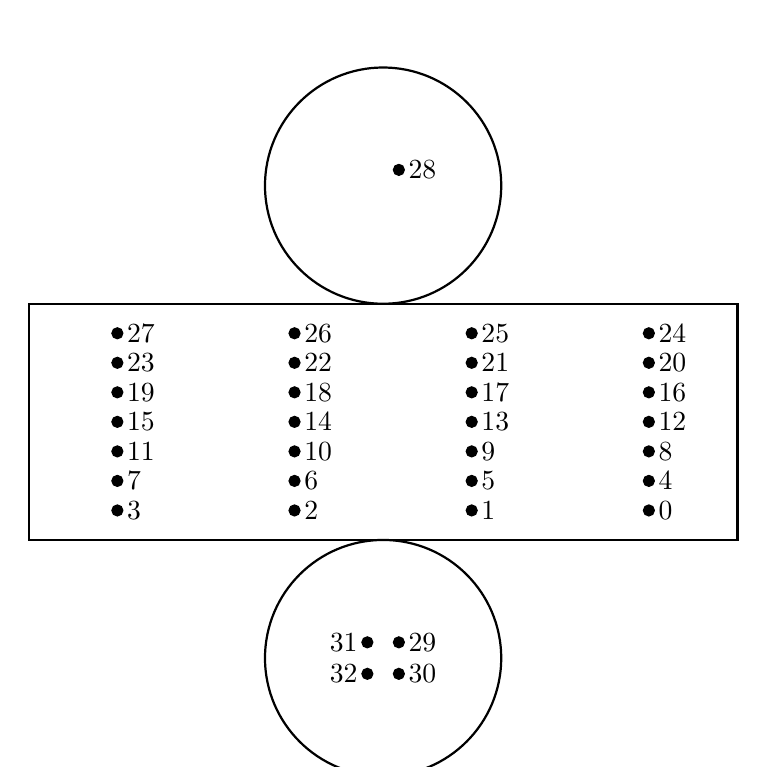
\begin{tikzpicture}
\draw[thick] (-4.5, -1.5) rectangle (4.5, 1.5);
\draw[thick] (0, 3) circle (1.5cm);
\draw[thick] (0, -3) circle (1.5cm);
\filldraw[black] (3.375, -1.125) circle (2pt) node[anchor=west]{0};
\filldraw[black] (3.375, -0.75) circle (2pt) node[anchor=west]{4};
\filldraw[black] (3.375, -0.375) circle (2pt) node[anchor=west]{8};
\filldraw[black] (3.375, 0) circle (2pt) node[anchor=west]{12};
\filldraw[black] (3.375, 0.375) circle (2pt) node[anchor=west]{16};
\filldraw[black] (3.375, 0.75) circle (2pt) node[anchor=west]{20};
\filldraw[black] (3.375, 1.125) circle (2pt) node[anchor=west]{24};
\filldraw[black] (1.125, -1.125) circle (2pt) node[anchor=west]{1};
\filldraw[black] (1.125, -0.75) circle (2pt) node[anchor=west]{5};
\filldraw[black] (1.125, -0.375) circle (2pt) node[anchor=west]{9};
\filldraw[black] (1.125, 0) circle (2pt) node[anchor=west]{13};
\filldraw[black] (1.125, 0.375) circle (2pt) node[anchor=west]{17};
\filldraw[black] (1.125, 0.75) circle (2pt) node[anchor=west]{21};
\filldraw[black] (1.125, 1.125) circle (2pt) node[anchor=west]{25};
\filldraw[black] (-3.375, -1.125) circle (2pt) node[anchor=west]{3};
\filldraw[black] (-3.375, -0.75) circle (2pt) node[anchor=west]{7};
\filldraw[black] (-3.375, -0.375) circle (2pt) node[anchor=west]{11};
\filldraw[black] (-3.375, 0) circle (2pt) node[anchor=west]{15};
\filldraw[black] (-3.375, 0.375) circle (2pt) node[anchor=west]{19};
\filldraw[black] (-3.375, 0.75) circle (2pt) node[anchor=west]{23};
\filldraw[black] (-3.375, 1.125) circle (2pt) node[anchor=west]{27};
\filldraw[black] (-1.125, -1.125) circle (2pt) node[anchor=west]{2};
\filldraw[black] (-1.125, -0.75) circle (2pt) node[anchor=west]{6};
\filldraw[black] (-1.125, -0.375) circle (2pt) node[anchor=west]{10};
\filldraw[black] (-1.125, 0) circle (2pt) node[anchor=west]{14};
\filldraw[black] (-1.125, 0.375) circle (2pt) node[anchor=west]{18};
\filldraw[black] (-1.125, 0.75) circle (2pt) node[anchor=west]{22};
\filldraw[black] (-1.125, 1.125) circle (2pt) node[anchor=west]{26};
\filldraw[black] (0.2, 3.2) circle (2pt) node[anchor=west]{28};
\filldraw[black] (0.2, -2.8) circle (2pt) node[anchor=west]{29};
\filldraw[black] (0.2, -3.2) circle (2pt) node[anchor=west]{30};
\filldraw[black] (-0.2, -2.8) circle (2pt) node[anchor=east]{31};
\filldraw[black] (-0.2, -3.2) circle (2pt) node[anchor=east]{32};
\end{tikzpicture}
\caption{Injector location map for ID positions. Each location will feature a diffuser and collimator.}\label{fig:IDmap}
\end{figure}
Installing injectors at different heights throughout the detector will allow water parameters to be measured as a function of depth.

The OD system will consist primarily of diffusers, using bare hemispheres coupled to fibres, rather than the housed versions used for the ID system; 122 of these OD diffusers will be installed. The current design features 84 equally spaced around the barrel region. This results in 7 rows of 12 diffusers, with rows alternately offset from one another. This configuration is particularly advantageous as it matches the number of rows in the ID system, simplifying the installation of the fibre optic cables. Each end-cap would then feature 19 diffusers, again equally spaced across the surface. A diagram showing this layout is presented in \cref{fig:ODdiffmap}. Finally, 12 collimators will be installed in the OD, in suitable locations to achieve long path lengths such as across the end caps and up the side of the barrel. These collimators will be exactly the same as those installed in the ID.

\begin{figure}[h!]
\centering
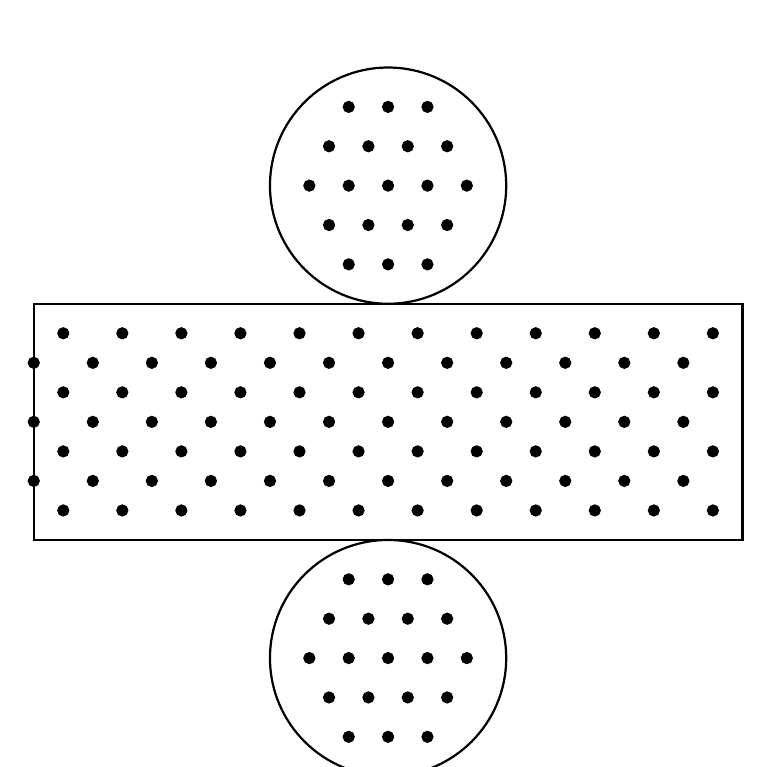
\begin{tikzpicture}
\draw[thick] (-4.5, -1.5) rectangle (4.5, 1.5);
\draw[thick] (0, 3) circle (1.5cm);
\draw[thick] (0, -3) circle (1.5cm);
%barrel locations
\foreach \x in {0,...,11}{
	\foreach \y in {0,...,6}{
		\ifodd \y \filldraw[black] (-4.5+\x*2*0.375, -1.125+\y*0.375) circle (2pt);
		\else \filldraw[black] (-4.5+0.375+\x*2*0.375, -1.125+\y*0.375) circle (2pt);
		\fi
		}
	}
%topcap
\foreach \y in {0,...,2}{
	\foreach \x in {0,...,2}{
		\filldraw[black] (-0.5+\x*0.5, 1.5+0.5+2*\y*0.5) circle (2pt);
		}
	}
\foreach \y in {0,...,1}{
	\foreach \x in {0,...,3}{
		\filldraw[black] (-0.75+\x*0.5, 1.5+2*0.5+2*\y*0.5) circle (2pt);
		}
	}
\foreach \x in {0,...,1}{
	\filldraw[black] (-1+\x*2, 3) circle (2pt);
	}
%bottom cap
\foreach \y in {0,...,2}{
	\foreach \x in {0,...,2}{
		\filldraw[black] (-0.5+\x*0.5, -1.5-0.5-2*\y*0.5) circle (2pt);
		}
	}
\foreach \y in {0,...,1}{
	\foreach \x in {0,...,3}{
		\filldraw[black] (-0.75+\x*0.5, -1.5-2*0.5-2*\y*0.5) circle (2pt);
		}
	}
\foreach \x in {0,...,1}{
	\filldraw[black] (-1+\x*2, -3) circle (2pt);
	}
\end{tikzpicture}
\caption{Injector location map for OD diffuser positions. Locations are approximate and dependent on PMT/WLS plate locations.}\label{fig:ODdiffmap}
\end{figure}

In order to illuminate the injectors, two separate systems will be employed. The first of these will be a system formed of either five or six picosecond pulsed laser sources, in the wavelength range 337-550 nm. This laser system will be used to illuminate all of the ID injectors, along with the 12 OD collimators. The OD diffusers on the other hand will be illuminated by an LED pulser system, utilising a series of 365~nm wavelength LEDs. Both of these systems will feature monitoring devices, so that the stability of the light sources can be monitored prior to convolution with detector parameters.

In total, including a laser diffuser ball and at least one spare channel, the lasers for the ID system will be required to couple to at least 80 channels. To accomplish this, dedicated fibre switching devices are required. A diagram giving an idea of the eventual laser and switch setup that would be used is given in \cref{fig:laserswitches}.
\begin{figure}[h]
\centering
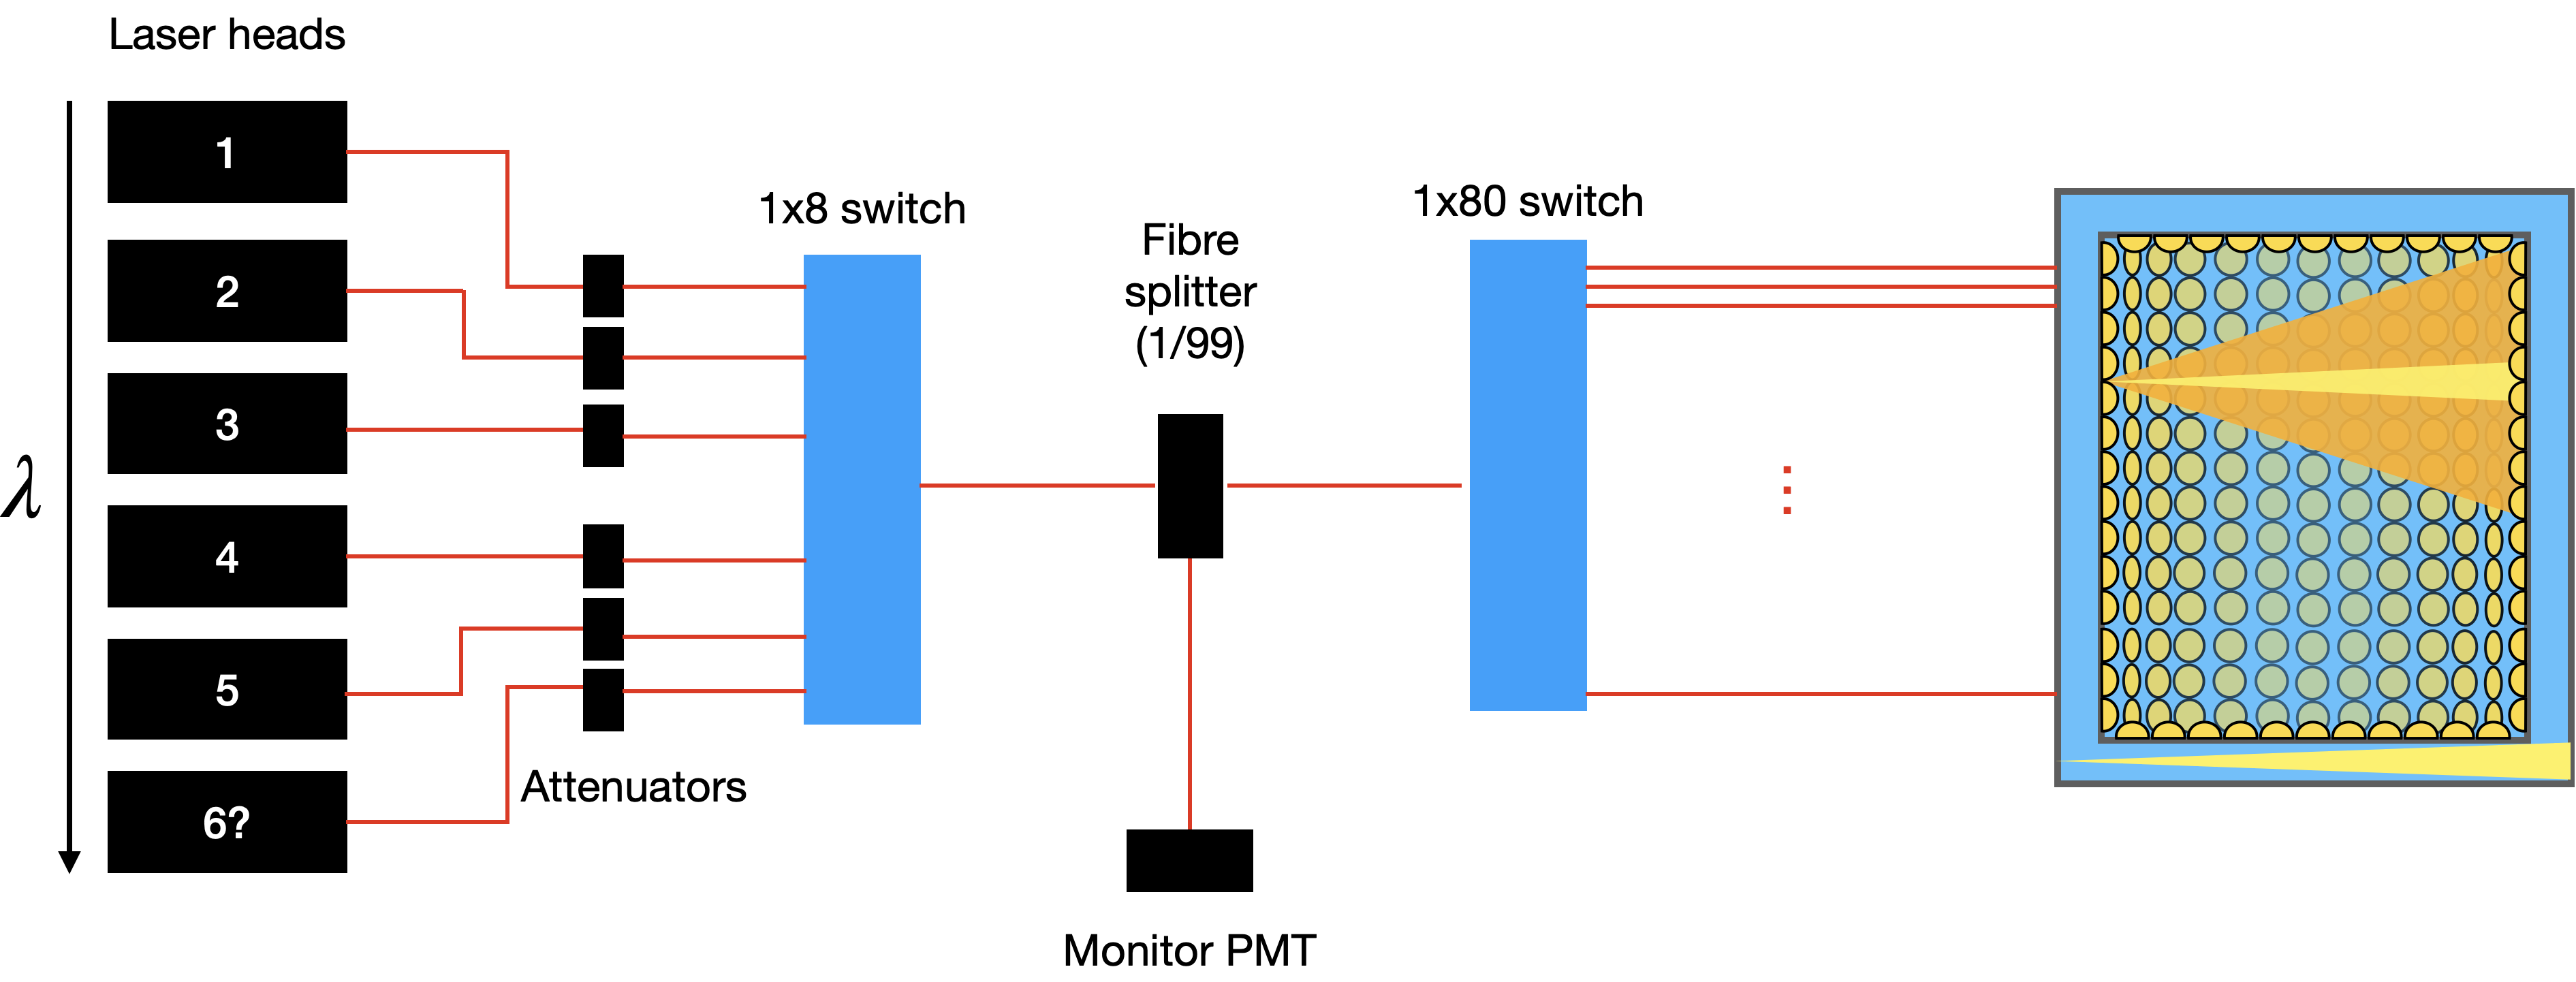
\includegraphics[width=0.9\textwidth]{switchConfiguration}
\caption{Diagram showing the likely setup for laser heads and fibre switchers.}\label{fig:laserswitches}
\end{figure}
These laser heads will be coupled into a single fibre using a 1-to-8 (hereafter denoted as 1x8) switch, after each individually passing through air-gap attenuators. While only five laser heads are initially planned, this allows the system to be expanded at a later date if required. Individual attenuators are used so that the power can be manually tuned for each laser, independently of the  others. The single fibre exiting the 1x8 switch can then connect to a fibre splitter with a 1/99 splitting. This allows 1\% of the laser power to be directed to a nearby monitor PMT, which will monitor laser power before coupling into the long fibres and without entangling water parameters from within the detector. The fibre with the remaining 99\% will go into a 1x80 switch, with the output going into the long fibres that extend down to the injectors.


\section{Laser System Specification}\label{sec:laser}
In order to perform the desired calibrations across a range of wavelengths, a system of at least five pico-second diode lasers is required. These must ideally be controlled from a single unit, to simplify communication and operation during regular data-taking and dedicated calibration runs. These lasers should be fibre-coupled, to avoid the need to direct an open beam into the fibre system. Avoiding any open beams is also preferable in terms of safety to both users of the system, and any nearby workers. The intended setup for this laser system, as described in \cref{sec:overview}, is shown in \cref{fig:laserswitches}. While the setup will begin with five lasers heads, the switch will allow for up to eight to be connected, giving the ability to expand the system at a later date if required.

As the large lengths of fibre required to transport light from the laser sources to injection points will result in both attenuation and dispersion of the signal, output power and pulse width from the lasers should be maximised and minimised, respectively. The studies performed to estimate the required pulse energy to illuminate 1\% of PMTs in spot region of each ID diffuser returned values of 5--10 pJ, with the maximum values at higher wavelengths. These studies are described in detail in \cref{sec:photonreq}. In certain scenarios, it will be necessary to inject more light into the detector than this. To account for this, a minimum pulse energy of 50 pJ was set for each laser wavelength. Coupling this with the requirement of short pulse widths, picosecond diode lasers were identified as the type of laser required. These lasers generally provide relatively high-powered pulses with pulse widths on the order of 1--100 ps.

Through our own market research and communicating with specialist laser suppliers, the preferred supplier identified for this system is PicoQuant \cite{bib:picoquant}, who manufacture high-powered pulsed picosecond diode lasers in a range of wavelengths. The Sepia PDL 828-L laser driver mainframe \cite{bib:laserdriver} allows for connection of up to eight laser drivers, which are all controlled from the single unit. This unit is capable of repetition frequencies with the internal oscillator of up to 80 MHz, though for the system in question triggering. The LDH Series of laser heads \cite{bib:laserhead} provide pulses below 100 ps in length, in the wavelength range 375 to 1990~nm, with the option to run in pulsed or continuous mode. As an option, they can be fibre coupled, which as described will be necessary for the system. The laser heads which best fit the system requirements are the LDH-D-C-375, LDH-D-C-390, LDH-D-C-440 and LDH-D-C-500 \cite{bib:picoquant}, which provide peak wavelengths of 375$\pm$5, 395$\pm$10, 440$\pm$10 and 500$\pm$10~nm respectively. In order to go below 375~nm the LDH-FA Series of laser heads \cite{bib:LDH} can be used, which is a fibre amplified laser head, providing pulses of less than 80~ps in width. For this specific case, the LDH-P-FA-355 with peak wavelength at 355$\pm$1~nm would be used. All of these laser heads fulfil the requirement of at least 50 pJ energy per pulse.

From this market research, it became clear that PicoQuant are the only company selling products that match the specification of both short pulse widths and high power. Several other companies which make picosecond diode lasers were contacted, but ultimately did not reach the power requirements. They are also fairly unique in the ability to control multiple laser heads with a single unit, whereas most commercial options need a single control unit per laser.


\section{Fibre Lab Measurements}

In order to make an informed decision on the optimal fibre optic cables to use for the LI system in HK, a series of measurements were made of the properties of the candidate fibres chosen. This section describes the fibre test stand setup at University of Liverpool, along with the measurements made of the candidate fibres, before discussing the decision on which fibres to use.

For the fibres to be suitable for use in the LI system, there are a series of requirements. These are:
\begin{itemize}
\item The fibre should be capable of transporting light of wavelengths in the range 337--550~nm.
\item The attenuation of the input signal across the full length of fibre should be minimised.
\item The dispersion of the input signal across the full length of fibre should be minimised.
\end{itemize}

Six different fibre types from Thorlabs were considered, to cover a range of options. Four of these were step-index fibres; two wide-core fibres (FP200URT \cite{bib:fp200urt} and FP400URT \cite{bib:fp400urt}) and two narrow-core fibres (FG050UGA \cite{bib:fg050uga} and FG105UCA \cite{bib:fg105uca}) were chosen. The remaining two candidates were graded-index fibres (GIF50C \cite{bib:gif50c} and GIF50D \cite{bib:gif50d}). Graded-index fibres were tested as it was expected that they would be required to limit dispersion of input signals across the full fibre length. It was particularly important to test the graded-index fibres as they are primarily for communications applications, and as such are only specified for operation above 800~nm. The main specifications of each fibre type are summarised in \cref{tab:fibres}. GIF50C and GIF50D have almost the same specifications, with the only difference being the available bandwidth.
\begin{table}[h]
\centering
\begin{tabular}{llccc}
\toprule
Fibre	   & Type   		  & Core \diameter [$\mu$m] &  NA 	  &  Transmission region [nm]\\ \midrule
FG050UGA   &  Step-index      &           \phantom{0}50  			&  0.22   &   250-1200       \\
FG105UCA   &  Step-index      &           105  			&  0.22   &   250-1200       \\
FP200URT   &  Step-index      &           200  			&  0.50   &   300-1200       \\
FP400URT   &  Step-index      &           400  			&  0.50   &   300-1200      \\
GIF50C     &  Graded-index    &           \phantom{0}50  			&  0.20	  &   800-1600       \\
GIF50D     &  Graded-index    &           \phantom{0}50 			&  0.20   &   800-1600      \\ \bottomrule
\end{tabular}
\caption{Fibre types used for initial testing in lengths of 1~m and 35~m.}\label{tab:fibres}
\end{table}
Preliminary measurements were performed with all six fibre types listed, and these results were used to make an informed choice on which should be investigated more thoroughly.


\subsection{Fibre Test Stand}\label{sec:meas:sub:stand}

All fibre measurements were performed using the fibre test stand in the Particle Physics Optical Laboratory at the University of Liverpool. Two different types of light sources are available for testing; the first of these is a Picoquant Sepia PDL 828-L laser driver \cite{bib:laserdriver}, powering a LDH-D-C-375M laser head \cite{bib:laserhead}, with a peak wavelength of 371~nm. This is a pulsed laser source with a pulse width of $\sim$50~ps, and repetition rate up to 80~MHz. The candidate fibres couple directly to the laser head using an FC/PC connector. The second set of light sources was a series of LEDs, covering wavelengths from 365~nm up to 595~nm. These are run in DC mode, and were used primarily to make attenuation measurements over the range of wavelengths relevant for the LI system. In order to connect the FC/PC connector on a candidate fibre to a surface-mounted LED, custom connectors were 3D printed.

Two different detection methods for the fibre transmitted light are available. To measure power output, a Thorlabs PM100USB \cite{bib:opm} power meter is used, with an S150C sensor \cite{bib:opmsensor} connected. For timing measurements, the fibres are connected to a Hamamatsu H10721-210 PMT \cite{bib:hpmt}, which is read out by a Tektronix MSO54 oscilloscope \cite{bib:scope}. Fibres are coupled to either read-out method via FC/PC connection such that, in the case of the laser, there are no bare beams in the lab. To ensure light tightness and as an additional safety measure, all light sources and detectors are housed within a dark box, with no connections made outside. Larger fibre reels are kept outside due to their size, with a port used to bring the ends inside for connection. An image of the setup is shown in \cref{fig:fibreteststand}.

\begin{figure}[h]
\centering
\includegraphics[width=\textwidth]{fibreTestStand}
\caption{Fibre test stand in the optical lab at University of Liverpool.}\label{fig:fibreteststand}
\end{figure}

\subsection{Preliminary Measurements}

In order to narrow down the choice of fibre optic cable, all six options listed in \cref{tab:fibres} were purchased, in lengths of 1~m and 35~m. This is much shorter than the fibres that will be needed for Hyper-K; full length fibres were not used due to supplier issues. The length of cables which could be cut was limited by the size of the building used for production, as cold weather conditions during winter in the US at the time of ordering prevented them from being cut outside. Rather than delay the measurements, the decision was taken to start preliminary measurements of attenuation and dispersion with the lengths that were available.

\subsubsection{Testing}\label{sec:meas:sub:init:sub:test}

Due to the early stage at which these measurements were made, the laser module described in \cref{sec:meas:sub:stand} had not yet been set up. Instead, preliminary measurements of both attenuation and dispersion were made using a pulsed 385~nm LED, operated by an early design of the LED pulser board that will be used for the OD LED system. In all tests, the 35~m lengths of fibre were left on the reels. This was both to remove cladding modes, as well as just to simplify the tests and not have to unwind this length of fibre around the lab. The 1~m fibres were also coiled to remove cladding modes as much as possible, though with such a short length the amount this could be done was limited.

To calculate dispersion of the signal across the fibre length, the width of the PMT signal pulse was measured for both lengths of each fibre. The pulse width is defined as the time elapsed while the voltage is at greater than 50\% of the peak. A total of 20,000 measurements were made for each set to estimate the uncertainty. Subtracting these values in quadrature obtains the amount of dispersion observed. The pulse widths at both lengths and calculated dispersion values for each fibre are presented in \cref{tab:dispinit}.
\begin{table}[h]
\centering
\begin{tabular}{lccc}
\toprule
Fibre	   & Pulse width at 1~m [ns]  & Pulse width at 35~m [ns] &  Dispersion [ns]		\\ \midrule
FG050UGA   &  $3.486\pm0.111$	      &  $4.207\pm0.305$         &  $2.355\pm0.569$     \\
FG105UCA   &  $3.734\pm0.075$	      &  $4.841\pm0.205$ 		 &  $3.081\pm0.335$     \\
FP200URT   &  $3.809\pm0.045$	      &  $5.117\pm0.158$	   	 &  $3.416\pm0.242$     \\
FP400URT   &  $4.329\pm0.054$	      &  $5.252\pm0.116$ 		 &  $2.974\pm0.219$     \\
GIF50C     &  $3.453\pm0.103$    	  &  $3.867\pm0.260$ 	     &  $1.741\pm0.613$     \\
GIF50D     &  $3.407\pm0.101$		  &  $3.899\pm0.213$ 		 &  $1.896\pm0.509$     \\ \bottomrule
\end{tabular}
\caption{Pulse width and dispersion values for initial fibre measurements, using a 385~nm pulsed LED source.}\label{tab:dispinit}
\end{table}
The results shown here are mostly unsurprising. As expected, the two graded-index fibres show the smallest amount of dispersion; this is exactly the reason they were added for consideration. For the first three step-index fibres, the dispersion increases with increased core diameter. However, it can be seen that the FP400URT, which has the largest core diameter, actually has a smaller amount of dispersion than the FP200URT. The typical rise time of a 50~cm PMT is quoted to be 5~ns \cite{bib:hkpmt}, so the fact that the pulse widths for all fibres but FP400URT are below this is a good sign.

The same set-up was also used to make preliminary measurements of attenuation in the fibres. As this was an early version of the fibre test stand, an optical power meter was not used. Instead, the area under the curve of each recorded pulse was used as a proxy, as this is proportional to the total charge collected by the PMT per pulse. Again, 20,000 measurements for each fibre sample were taken, and the results for this are presented in \cref{tab:attinit}.
\begin{table}[h]
\centering
\begin{tabular}{lccc}
\toprule
Fibre	   & 1~m [nVs]  & 35~m [nVs] &  Transmittance [\%]	\\ \midrule
FG050UGA   &  $\phantom{0}1.86\pm0.23$     &   $\phantom{0}0.75\pm0.23$     & \phantom{0}$40.3\pm13.3$     \\
FG105UCA   &  $\phantom{0}7.16\pm0.62$	    &   $\phantom{0}4.17\pm0.28$    & $58.2\pm6.4$     \\
FP200URT   &  $16.53\pm0.99$				&  	$\phantom{0}9.59\pm0.74$  	& $58.0\pm5.7$     \\
FP400URT   &  $23.56\pm1.14$    			&   $19.24\pm0.94$	 			& $81.7\pm5.6$     \\
GIF50C     &  $\phantom{0}4.61\pm0.69$     &   $\phantom{0}4.09\pm0.59$	 	& \phantom{0}$88.7\pm18.4$     \\
GIF50D     &  $\phantom{0}2.39\pm0.57$     &   $\phantom{0}0.56\pm0.24$     & \phantom{0}$23.4\pm11.5$    \\ \bottomrule
\end{tabular}
\caption{Area-under-curve measurements from oscilloscope for 1~m and 35~m fibres, with calculated transmittance values.}\label{tab:attinit}
\end{table}
Again, the results shown here are unsurprising for the step-index fibres, with the transmittance increasing with increased core diameter. It can also be seen that the recorded values through the 1~m patch cable increase with increasing core diameter; this shows the difficulty of coupling particularly narrow-core fibres to an LED, which generally have a wide opening-angle for the light profile. The results obtained for the two graded-index fibres are seen to be very different, which is potentially related to the different bandwidths they're designed for, and the fact they're not specified for a wavelength range below 800~nm. The amount of charge collected from a 1~m fibre for either of these types is again small due to them having a 50 $\mu$m core diameter, and suggests as expected that narrow-core fibres are not suitable for the OD LED pulser system.

\subsubsection{Results}

The results from these initial tests suggest that different fibre types will need to be employed for the ID laser and OD LED systems. For the OD LED system, where coupling the fibre to the LED and maximising light transmission is important, a wide-core fibre should likely be chosen. The FP400URT fibre showed the best transmission and input light acceptance, so this is the candidate that was favoured. For the laser system timing is more important; the dispersion measurements suggested that the graded-index GIF50C and GIF50D fibres were the best candidates here.

As this was a preliminary version of the fibre test stand, and measurements were carried out with fibre lengths significantly shorter than what will actually be installed into Hyper-K, the decision was initially taken to purchase three candidate fibres for further testing. These were FP400URT, GIF50C and GIF50D. Based on estimates of the length required, reels of 40~m and 105~m length were purchased for each of these fibre types. However, it was later understood that the feed-throughs for the injectors would use an FG105UCA patch cable. In order to not add extra inefficiencies to the system in coupling different fibres to one another, the ideal scenario would be to use this fibre for the laser system. A reel of 105~m for this was also purchased and tested, with results for all four primary candidate fibres described together in the following sections for simplicity.


\subsection{Attenuation Measurements}

\subsubsection{Method}\label{sec:fibre:sub:att:sub:method}

The full laser setup for the HK LI system will feature a minimum of five laser heads, over a range of wavelengths spanning UV to visible. In order to confirm whether attenuation in the candidate fibres is of an acceptable level across multiple wavelengths, LEDs across a series of wavelengths were used for these tests. Those were: 365, 395, 415, 465, 496, 525 and 560~nm. As timing is not relevant to attenuation measurements, and to ensure results were valid by initially getting enough light into the fibres, these LEDs were powered with a DC source.

Measurements were made of the output power from fibres of length 1, 2, 37, 42, 77, 107 and 147~m, where some of these lengths were formed by coupling together multiple fibres of shorter length, and all lengths above 1~m featured two 1~m patch cables in the setup. To connect fibres together, FC/PC to FC/PC mating sleeves were used, which are quoted to have $<0.5$~dB insertion loss \cite{bib:matingsleeve}. As a 40~m length of FG105UCA fibre was not ordered, the measurements for this were done at slightly altered lengths. Power measurements were made using an optical power meter, as described in \cref{sec:meas:sub:stand}. The longer reels of fibre were purchased without tubing, and it was observed during data taking that there was some level of light leakage into the fibres, causing non-zero readings when the LEDs were not powered. To mitigate this, all measurements were performed with the reels of fibre that were too big to fit inside the dark box wrapped in black sheet.

The power observed after transmission through a fibre of length $x$ can be written as
\begin{eqnarray}
P = P_0\exp^{-\lambda x},
\end{eqnarray}
where $P$ is the observed power after traversing the fibre, $P_0$ is the initial power, and $\lambda$ is the coefficient of attenuation, describing how much attenuation occurs per unit length. Taking the natural logarithm of this,
\begin{eqnarray}
\ln P = -\lambda x + \ln P_0,
\end{eqnarray}
allows a linear fit to be made to data, where the gradient is the coefficient of attenuation, and the y-intercept the log of the input power. The fitted attenuation coefficient can then be used to calculate attenuation in dB for a given fibre length, where in this case a length of 150~m is used:
\begin{eqnarray}
\text{Attenuation (dB/150~m)} = \frac{10}{\ln 10}\times 150 \times \lambda.
\end{eqnarray}

\subsubsection{Results}\DIFaddbegin \label{sec:fibre:sub:att:sub:results}
\DIFaddend As a first check of the measurement system, the calculated attenuation values for the FP400URT fibre were compared to those provided in the fibre specifications by Thorlabs. This comparison can be seen in \cref{fig:fp400compar}, and shows generally good agreement between the two. Values of attenuation stay below 10~dB until just above 400~nm, where the amount of attenuation increases sharply. At the minimum wavelength of 365~nm, attenuation of over 20~dB is observed, suggesting that attenuation values in the UV range will likely be the driving factor for deciding on a fibre type.

\begin{figure}[h]
\centering
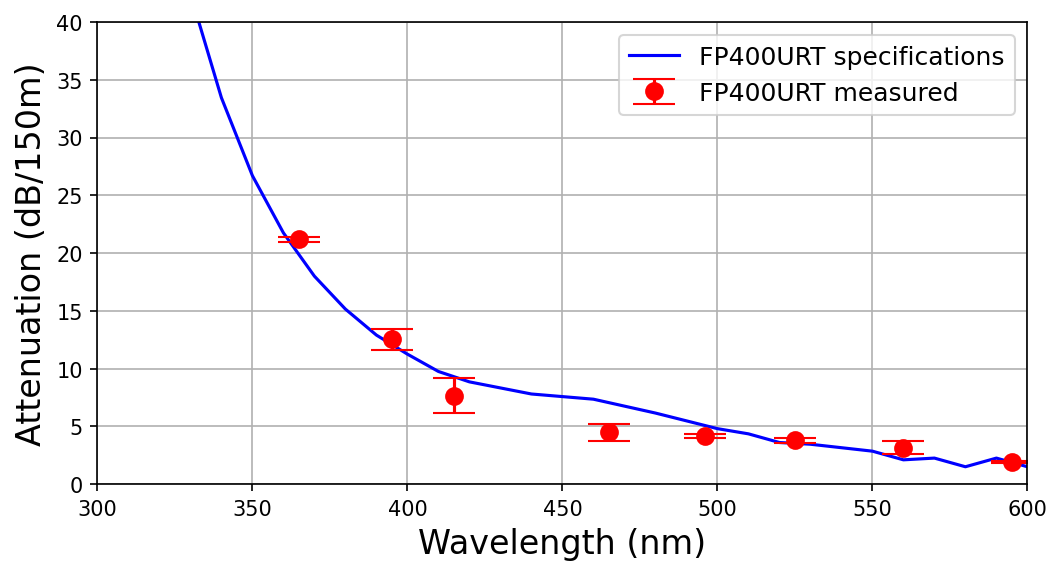
\includegraphics[width=0.8\textwidth]{FP400Compar.png}
\caption{Measured attenuation scaled to 150~m length as a function of wavelength for the FP400URT fibre, compared to specifications from Thorlabs \cite{bib:fp400urt}.}\label{fig:fp400compar}
\end{figure}

The full results for all fibre types are presented in \cref{fig:attenall}, with all values of attenuation again scaled to what would be seen across 150~m of fibre. As was shown for the FP400URT fibre, the amount of attenuation observed in the fibres peaks at the lowest wavelength scanned, 365~nm. At this value there is a large range of values observed, with the FG105UCA fibre exhibiting the lowest attenuation at under 15~dB. Conversely, the two graded index fibres show much greater attenuation. The spread of values at 395~nm is much reduced, with the two graded-index fibres instead exhibiting lower attenuation here. Above 400~nm, the FG105UCA fibre is seen to consistently exhibit higher attenuation than the other fibres, though in all cases is still below 10~dB.
\begin{figure}[h]
\centering
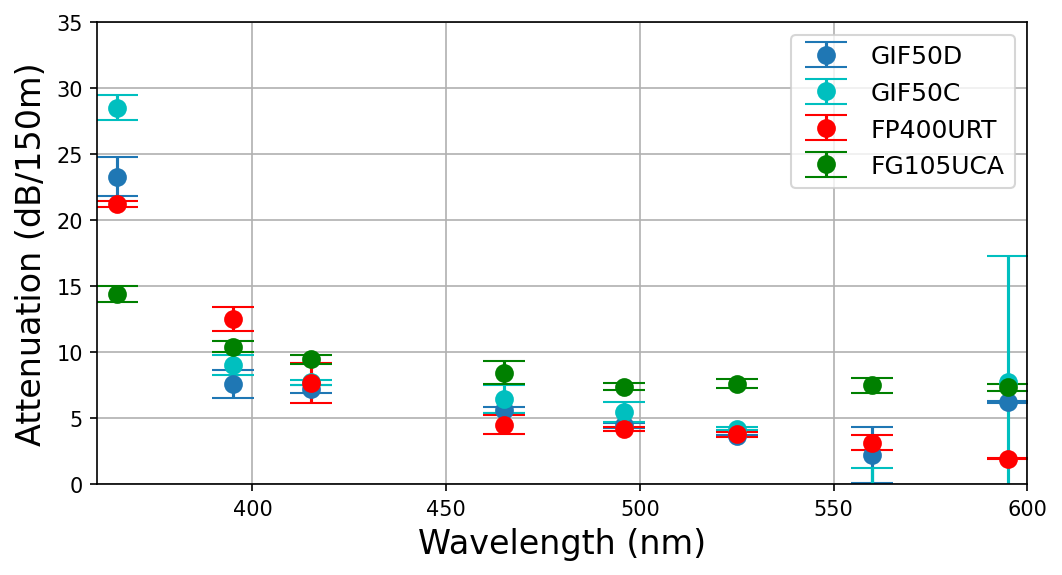
\includegraphics[width=0.8\textwidth]{AttenAll.png}
\caption{Measured attenuation scaled to 150~m length for all four candidate fibre types, as a function of wavelength.}\label{fig:attenall}
\end{figure}
These results suggest that FG105UCA is the optimal fibre type to use, in terms of attenuation. Although it exhibits higher attenuation in the visible range, there is significantly less observed in the UV range, whereas the other fibre options start to peak sharply in attenuation here. As lower wavelengths of light have been previously observed to be more sensitive to changes in water parameters \cite{bib:skgd2}, prioritising lower attenuation in this region should be preferred.

Performing these tests also provided an opportunity to become familiar with handling the fibres. As was mentioned in \cref{sec:fibre:sub:att:sub:method}, the long reels of fibre that were purchased for these tests were done so without tubing, which is generally added in order to protect the fibres. Along with the issues of light leakage previously discussed, during testing it was found that the narrow-core fibres were particularly fragile, with two being broken in the process. The FP400URT fibre however was seen to be far more robust and light-tight. This is attributed to its hard polymer cladding and Tefzel (Teflon-based) coating, as opposed to the clear acrylate used for the graded-index and FG105UCA fibres. \DIFdelbegin \DIFdel{Orders of fibre types other than FP400URT will require tubingwhen ordered for the safety of the system.
}\DIFdelend \DIFaddbegin \DIFadd{Despite this, for safety and light-tightness both types of fibres will use furcation tubing. The majority of fibres will be tubed using the Thorlabs FT030-BK black tubing \mbox{%DIFAUXCMD
\cite{bib:ft030bk}}\hskip0pt%DIFAUXCMD
. This is the same tubing using on the fibres in the UK Light Injection (UKLI) system in Super-K, so it is known to be compatible with both ultra-pure and gadiated water. Short patch fibres used inside the LED pulser crate (described further in \mbox{%DIFAUXCMD
\cref{sec:lengths:sub:len:sub:patch}}\hskip0pt%DIFAUXCMD
) will use different colours, associated with the different total fibre lengths that each pulser is connected to.
}\DIFaddend 

\subsection{Dispersion Measurements}

\subsubsection{Method}

Similarly to the attenuation measurements described above, by the time the full lengths of fibre had been ordered in, the full fibre test stand had been commissioned. Importantly, this included setup of the laser system described in \cref{sec:meas:sub:stand}, which was used as the light source for these measurements. Instead of the $\mathcal{O}$(ns) input pulse provided by the pulsed LEDs in \cref{sec:meas:sub:init:sub:test}, the laser delivers a pulse of width $\sim50$ ps, meaning measurements would not be limited by this.

Various lengths of each fibre were connected in turn to the laser head, in the same way as in \cref{sec:fibre:sub:att:sub:method}. However, due to breakage in the attenuation testing GIF50C was not included in these tests. To make timing measurements, the fibres were connected to the PMT, where the signal was visualised on the oscilloscope. Across 20,000 recorded pulses, measurements were made of the pulse width, negative rise time and negative fall time. Pulse widths were again defined as the time above 50\% of the peak voltage, while rise and fall times were defined as the time between 20\% and 80\%, or vice versa.

In making these measurements, another limitation of the setup became apparent; it was clear from initial measurements that the measured pulse width and rise time were highly dependent on the amount of light detected by the PMT. This was understood to be a limitation caused by the rise time of the PMT; shorter fibres which would deliver more light due to decreased attenuation exhibited longer pulse widths, as the PMT response was not quick enough. In order to get around this, the measurement approach was modified. For each length of fibre tested, the laser intensity was adjusted such that the output pulse would deliver approximately the same peak voltage each time. This should ensure that the rise time of the PMT had no impact on the timing measurements.

Another issue was encountered with this setup. When making measurements with the 1~m patch cable, large tails in the pulses were observed. An example of this for the FP400URT 1~m cable is shown in \cref{fig:fp400urt1m}. Here, negative rise time and negative fall time are labelled as fall time and rise time, respectively, due to the inverted nature of the pulse.
\begin{figure}[h]
\centering
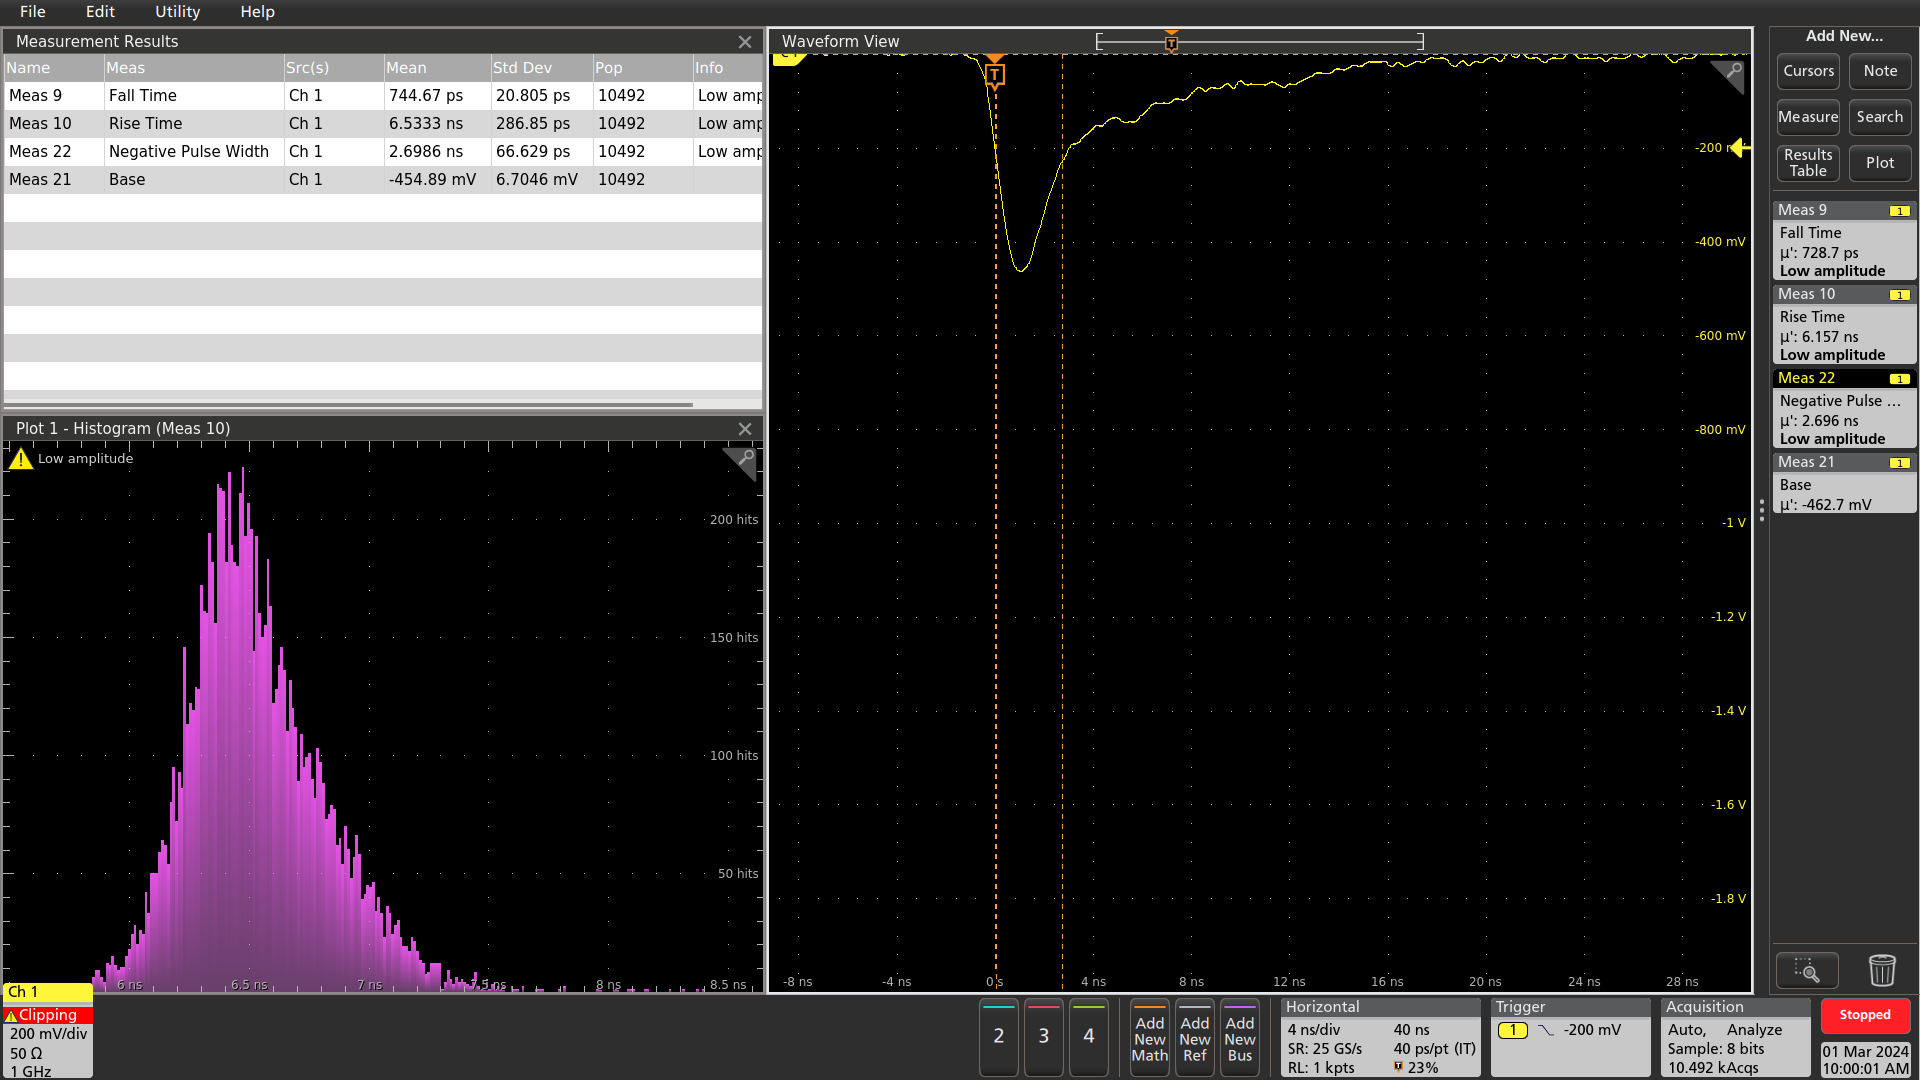
\includegraphics[width=\textwidth]{FP400URT_1m_1.png}
\caption{Scope trace and associated measurements for a 1~m FP400URT patch cable, showing the long falling tail observed.}\label{fig:fp400urt1m}
\end{figure}
It can be seen that the very slowly falling tail results in a negative fall time of $6.53\pm0.29$~ns, despite a negative rise time of only $0.74\pm0.02$~ns. This results in a measured pulse width longer than those observed for longer fibre lengths, making dispersion incalculable. As the long tails diminish with increased fibre length, it is thought that they are caused by reflections at the fibre coupling faces. In order to not be affected by this, measurements instead focused on the negative rise time of pulses. Unfortunately this still makes dispersion incalculable, but at least gives a way to compare pulse timing for each fibre type.

\subsubsection{Results}\label{sec:fibre:sub:disp:sub:method}

The obtained rise time measurements for the three fibre types tested are given in \cref{fig:disprise}. As expected from the preliminary measurements, the fibre which exhibited the least increase in rise time was the graded-index, GIF50D, with an increase of $0.24\pm0.03$~ns. This is closely followed by FP400URT, which shows an overall increase of $0.34\pm0.03$~ns. A comparably higher increase is then observed for the FG105UCA fibre of $0.60\pm0.05$~ns.
\begin{figure}[h]
\centering
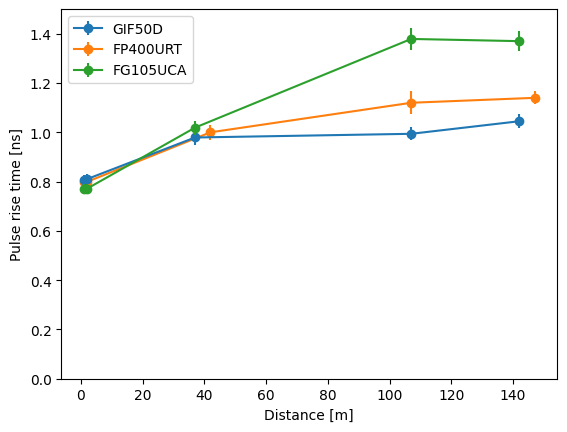
\includegraphics[width=0.6\textwidth]{RiseTimeOct24_zero.png}
\caption{Pulse rise time measurements for three candidate fibres, across a range of lengths.}\label{fig:disprise}
\end{figure}
An interesting observation in these measurements is that the rise time increase is relatively sharp over the first $\sim$50~m, but then plateaus toward the longest distances measured. This suggests that, should fibres be required to be longer than those tested, there should not be a substantial increase in rise time over what has already been observed. It should also be noted that, at the maximum distance of $\sim$140~m, the measured rise times for all fibres are smaller than the typical 50~cm PMT rise time of 5~ns \cite{bib:hkpmt}.

While these measurements give a good estimate of how timing will increase over large lengths for each fibre type, it will be important to confirm exact dispersion measurements for the chosen fibre type. As such, a high frequency readout system is currently in development, so that these measurements can be made at a later time.

\subsection{Fibre Choice}\label{sec:fibre:sub:choice}

Unfortunately, the results from both the attenuation and dispersion tests are diametrically opposed; while the graded index fibres performed best in terms of dispersion and pulse rise time increase, they exhibited the greatest amount of attenuation. The opposite is true for the FG105UCA fibre, with FP400URT performance in the middle for both tests, meaning there is not a single fibre type that is clearly preferred. Specific aspects and requirements of the two separate LI systems should be taken into account to make this choice.

Firstly, it is important to remember that the decibel scale is logarithmic, meaning that the $\sim$10~dB difference between the FG105UCA and FP400URT/GIF50D fibres observed at 365~nm represents an additional $\mathcal{O}$(10) times power loss. Therefore, the differences observed in attenuation are much greater than for the pulse width measurement, and as such the former should be prioritised as a basis for fibre decisions. While the GIF50D fibre showed the best results in terms of rise time increase, it showed significantly worse attenuation. Secondly, the ID injectors (and OD collimators) already have an internal patch fibre of FG105UCA. Coupling a wide-core fibre such as FP400URT into this narrow-core fibre will result in significant light loss at the connection point, and so should be avoided. Therefore, on balance, the FG105UCA narrow-core step-index fibre is judged to be the optimal choice for the laser system. However, the initial results for the 1~m patch cables given in \cref{tab:attinit} make it clear that coupling an LED to such a small core diameter fibre is difficult. As such, the choice for the OD LED system is the FP400URT fibre, which has a four times wider core and the next best attenuation results.



\section{Fibre Switching Device}\label{sec:switch}

\subsection{Overview}
As was mentioned in \cref{sec:overview}, the ID laser system will require dedicated fibre switching devices in order to couple all lasers to all possible channels. To that end, two potential companies that manufacture fibre switching devices were identified, and test devices in a 1x4 configuration were purchased for evaluation. From the first company, Agiltron \cite{bib:agiltron}, a single 1x4 device was purchased with FP400URT as the internal fibre. A second company, Weinert Industries \cite{bib:weinert} supplied two 1x4 devices; one of these contained FP400URT fibre, while the other used GIF50C. All three devices are controlled via USB. It should be noted that only two companies could be found that could supply these kinds of specialist devices.

\subsection{General Comparisons}

To understand the performance of the three test switches, power measurements were made comparing the output power from each of the four ports to a reference fibre of the same type. For the reference fibre measurements, two 1~m patch cables were coupled together to make a 2~m cable, with the total cable length of each of the switches being around this length.

Measurements were made using the 371~nm laser as the light source. The power meter was used to make measurements across 20,000 readings, where each of the four fibre outputs on a switch were selected and coupled to in turn. Power readings and calculated transmission percentages for the Agiltron FP400URT switch are given in \cref{tab:switchpower}.
\begin{table}[h]
\centering
\begin{tabular}{l|cc|cc|cc}
\toprule
\multirow{2}{*}{} & \multicolumn{2}{c|}{Agiltron FP400URT} & \multicolumn{2}{c|}{Weinert FP400URT} & \multicolumn{2}{c}{Weinert GIF50C} \\
			&	Power ($\mu$W) & \% of ref. & Power ($\mu$W) & \% of ref. & Power ($\mu$W) & \% of ref.\\ \midrule
Reference	& $9.58\pm0.01$	& 100  			 & $9.67\pm0.01$ & 100 			  & $9.69\pm0.01$ & 100 \\
Port 1		& $8.93\pm0.01$	& $93.11\pm0.14$ & $7.41\pm0.01$ & $76.64\pm0.13$ & $9.49\pm0.01$ & $98.09\pm0.20$ \\
Port 2		& $8.67\pm0.01$	& $90.55\pm0.14$ & $7.41\pm0.01$ & $76.64\pm0.13$ & $9.59\pm0.01$ & $98.83\pm0.20$ \\
Port 3		& $8.71\pm0.01$	& $91.06\pm0.14$ & $7.27\pm0.01$ & $75.18\pm0.13$ & $9.36\pm0.01$ & $96.70\pm0.20$ \\
Port 4		& $8.66\pm0.01$	& $90.50\pm0.14$ & $7.00\pm0.01$ & $72.39\pm0.13$ & $9.23\pm0.01$ & $95.30\pm0.20$ \\
\bottomrule
\end{tabular}
\caption{Power transmission across the 1x4 switching devices, with comparison to a reference cable of the same type as the device internal fibre.}\label{tab:switchpower}
\end{table}
The results obtained show generally good power transmission for all three devices tested, albeit with clearly better transmission for the Agiltron FP400URT and Weinert GIF50C than for the Weinert FP400URT. This may be in part due to the fact the fibre on the Weinert FP400URT is longer than the others (and the 2~m reference), measuring approximately 2.3~m in total. It should be noted here that, at least for the Weinert switches, any switch with more than four outputs is formed by daisy-chaining together 1x4 switches. For example, a 1x16 switch would be constructed by connecting the four output channels of a single 1x4 switch into the inputs of four additional 1x4 switches. Therefore for the required 1x6 and 1x80 switches, these losses will be experienced up to six times in total. It is unclear whether the Agiltron switch is constructed in the same manner.

The variation in output power between ports is also generally low across the devices, with a difference of 2.61\% for the Agiltron FP400URT, 4.25\% for the the Weinert FP400URT and 3.53\% for the Weinert GIF50C. These results suggest that the Agiltron device minorly outperforms the Weinert devices in terms of power variation across ports, whilst the Weinert GIF50C was best for transmission.

During ordering, setup and testing of these devices, we experienced very different degrees of assistance from the two companies. While this is not a quantifiable metric, it is none the less very important to keep in mind when making a decision for the full fibre system. The Agiltron switch arrived with no documentation on how to set up and run the device. The correct way of doing this was eventually understood out after several emails to the supplier. The Weinert switches on the other hand arrived with full documentation, along with a simple software package for operation. All email communication with them throughout the ordering and testing process has been very helpful, if somewhat slow at times.

The LI system is a critical component of the HK calibration programme, and will need to run for many years. It is crucial that support is available from the manufacturer of significant components such as the fibre optic switch, should anything go wrong during its lifetime. The experience of working with Weinert was significantly better, and this should be kept in mind when selecting which device to proceed with. In particular, should issues arise with hardware in the future, it would be significantly easier to deal directly with the manufacturer, rather than going through a third-party distributor as with Agiltron.


\subsection{Cross-talk Measurements}

While making the transmittance measurements shown in \cref{tab:switchpower} for the Agiltron device, it was noted that small non-zero readings were being made by the power meter whilst connected to ports that were not currently being illuminated. These persisted after turning off the laser and re-zeroing the power meter, and suggested some crosstalk between fibres. This is of course something that should be avoided, as only one injector should be illuminated within the tank at a time.

In order to confirm this was the case and measure the level of crosstalk for these devices, four power meters were set up, with one connected to each of the four ports on a switch, and all re-zeroed at the same time. A simple python script was used to loop through the four ports 1000 times, before stopping at each port in turn and taking readings for $\sim$10~s. This was repeated for runs of approximately 18 hours per fibre switching device. Data was analysed by stripping out data points from the rapidly varying periods, as well as the first and last point of each sustained period where the device may still have been switching and thus not illuminating the port for the entire time taken for one reading.

Data from this test is shown in \cref{fig:agifp400crosstalk,,fig:weinfp400crosstalk,fig:weingifcrosstalk} for the Agiltron FP400URT, Weinert FP400URT and Weinert GIF50C switches, respectively. Each of these shows data taken by the power meters when the port was a) illuminated and b) not illuminated. These plots show a subset of the full data-taking runs in order to better show the observed structure. \cref{fig:agifp400crosstalkon,fig:weinfp400crosstalkon,fig:weingifcrosstalkon}, which show the readings from illuminated ports, show a similar level of variation to the data presented in \cref{tab:switchpower}.
\begin{figure}[h!]
\centering
\begin{subfigure}{0.5\textwidth}
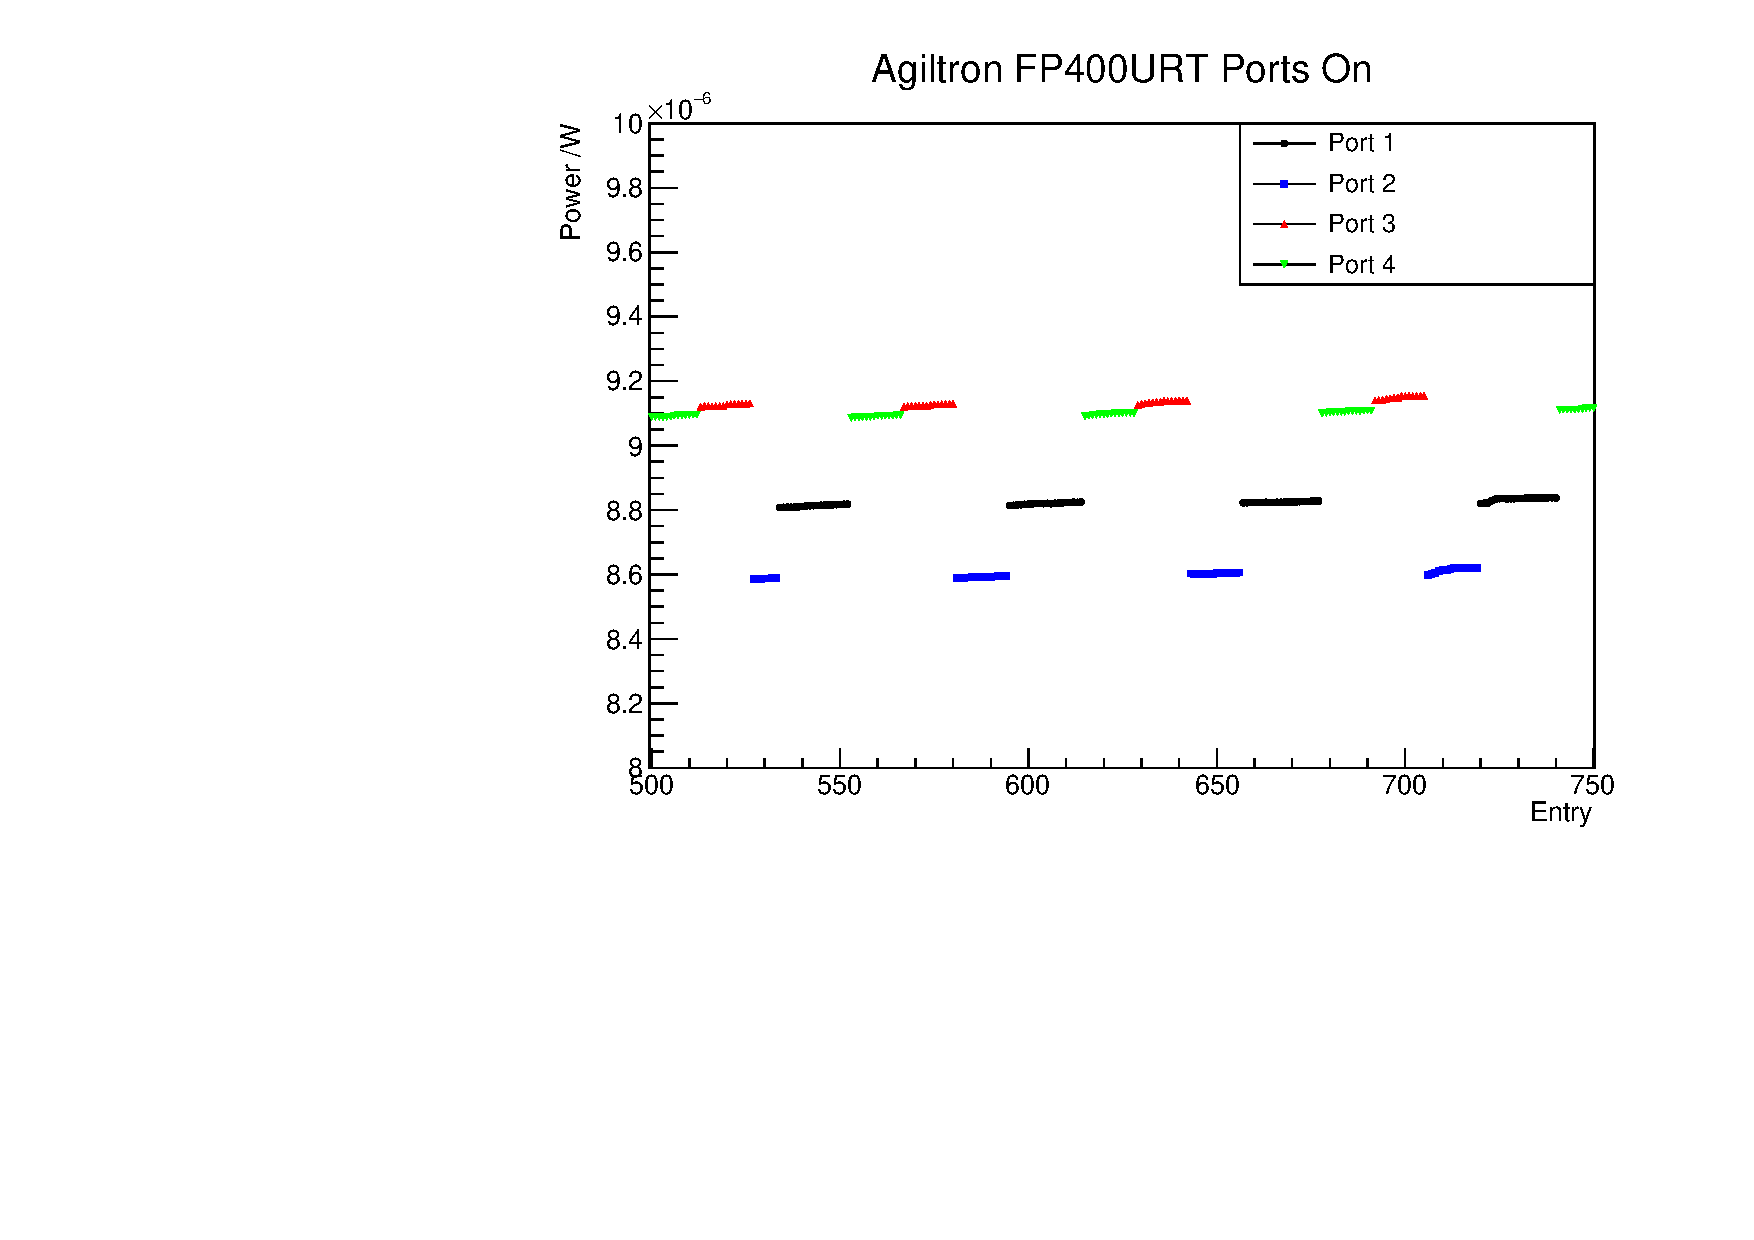
\includegraphics[width=\linewidth]{AgiltronFP400URTPortsOnZoom.pdf}
\subcaption{}\label{fig:agifp400crosstalkon}
\end{subfigure}%
\begin{subfigure}{0.5\textwidth}
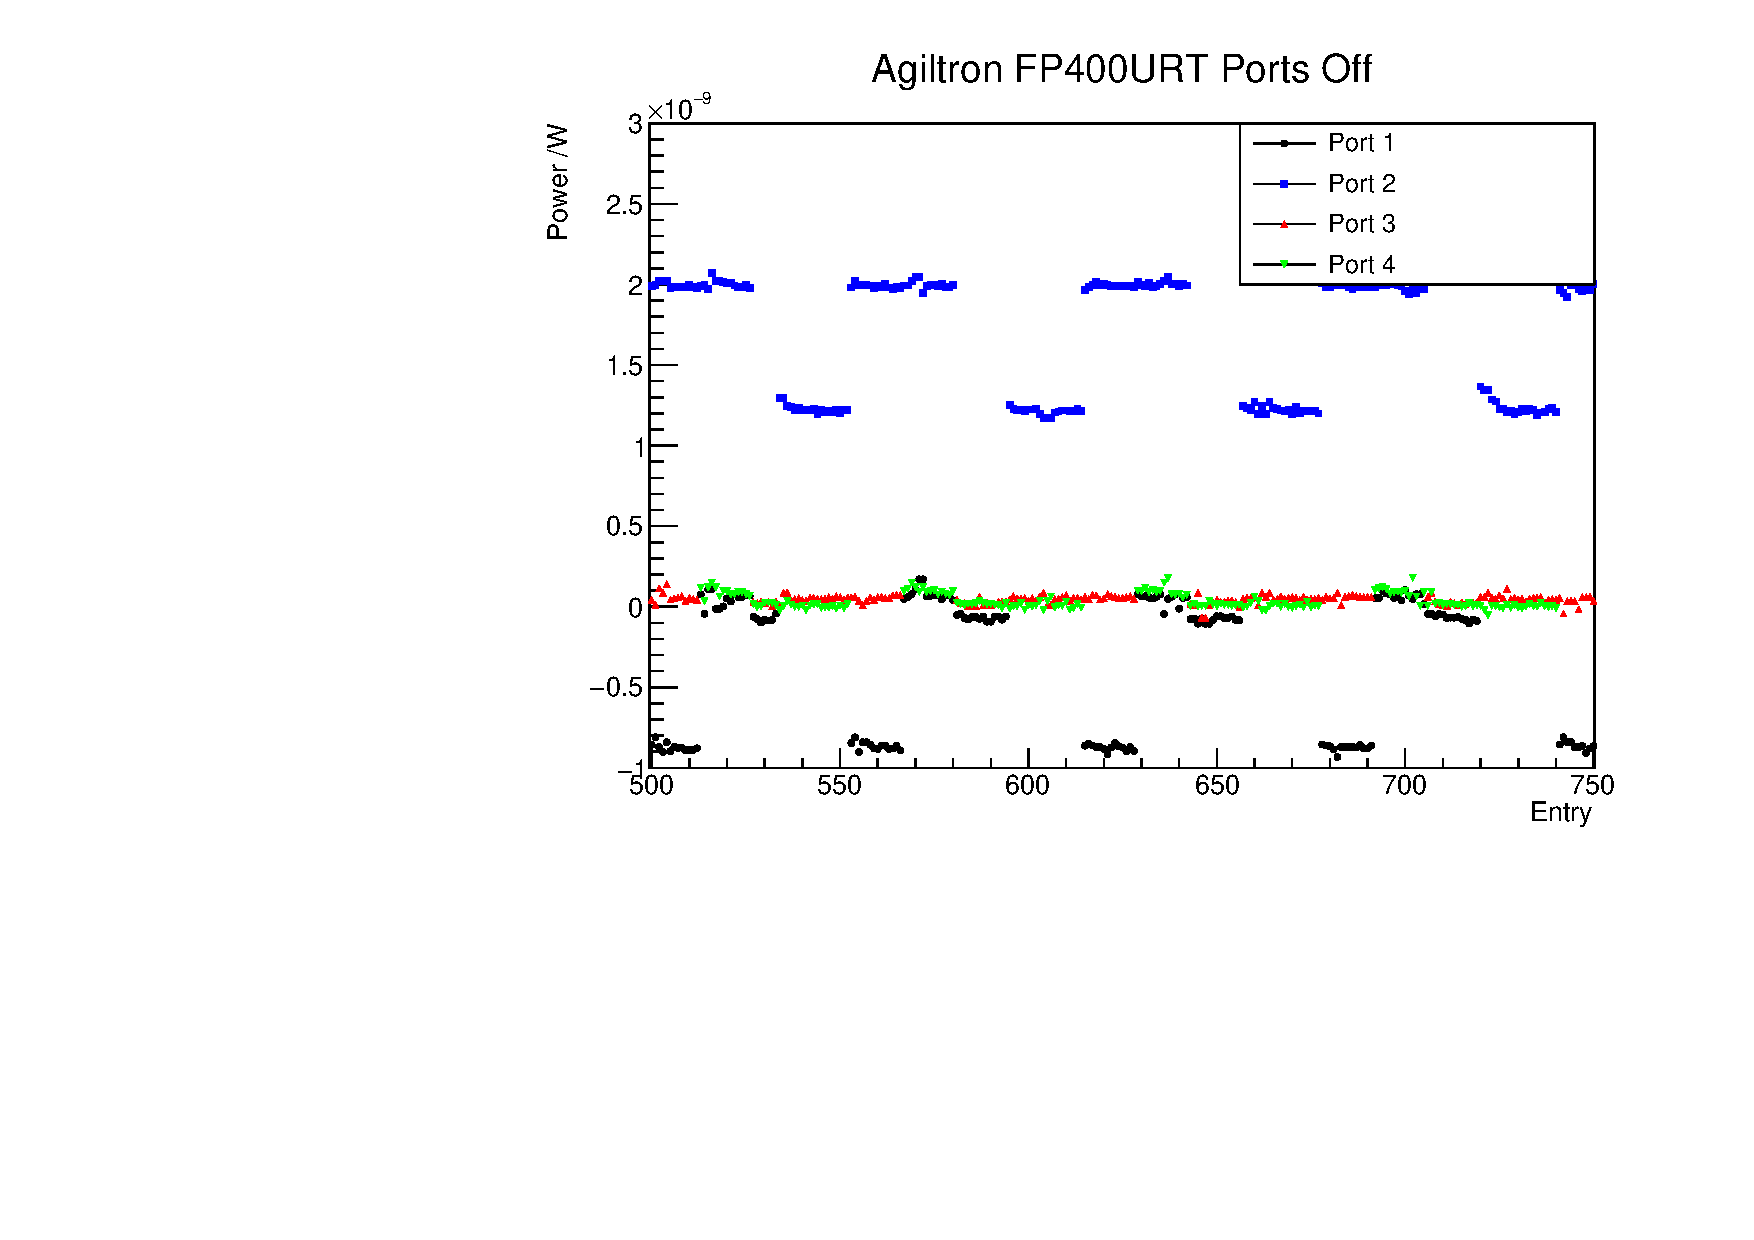
\includegraphics[width=\linewidth]{AgiltronFP400URTPortsOffZoom.pdf}
\subcaption{}\label{fig:agifp400crosstalkoff}
\end{subfigure}
\caption{Power meter readings from all four ports for the Agiltron FP400URT device, zoomed into a shorter period of data to better show structure. Data is shown for when ports are a) illuminated and b) not illuminated. Note the different y-axis scales.}\label{fig:agifp400crosstalk}
\end{figure}
\begin{figure}[h!]
\centering
\begin{subfigure}{0.5\textwidth}
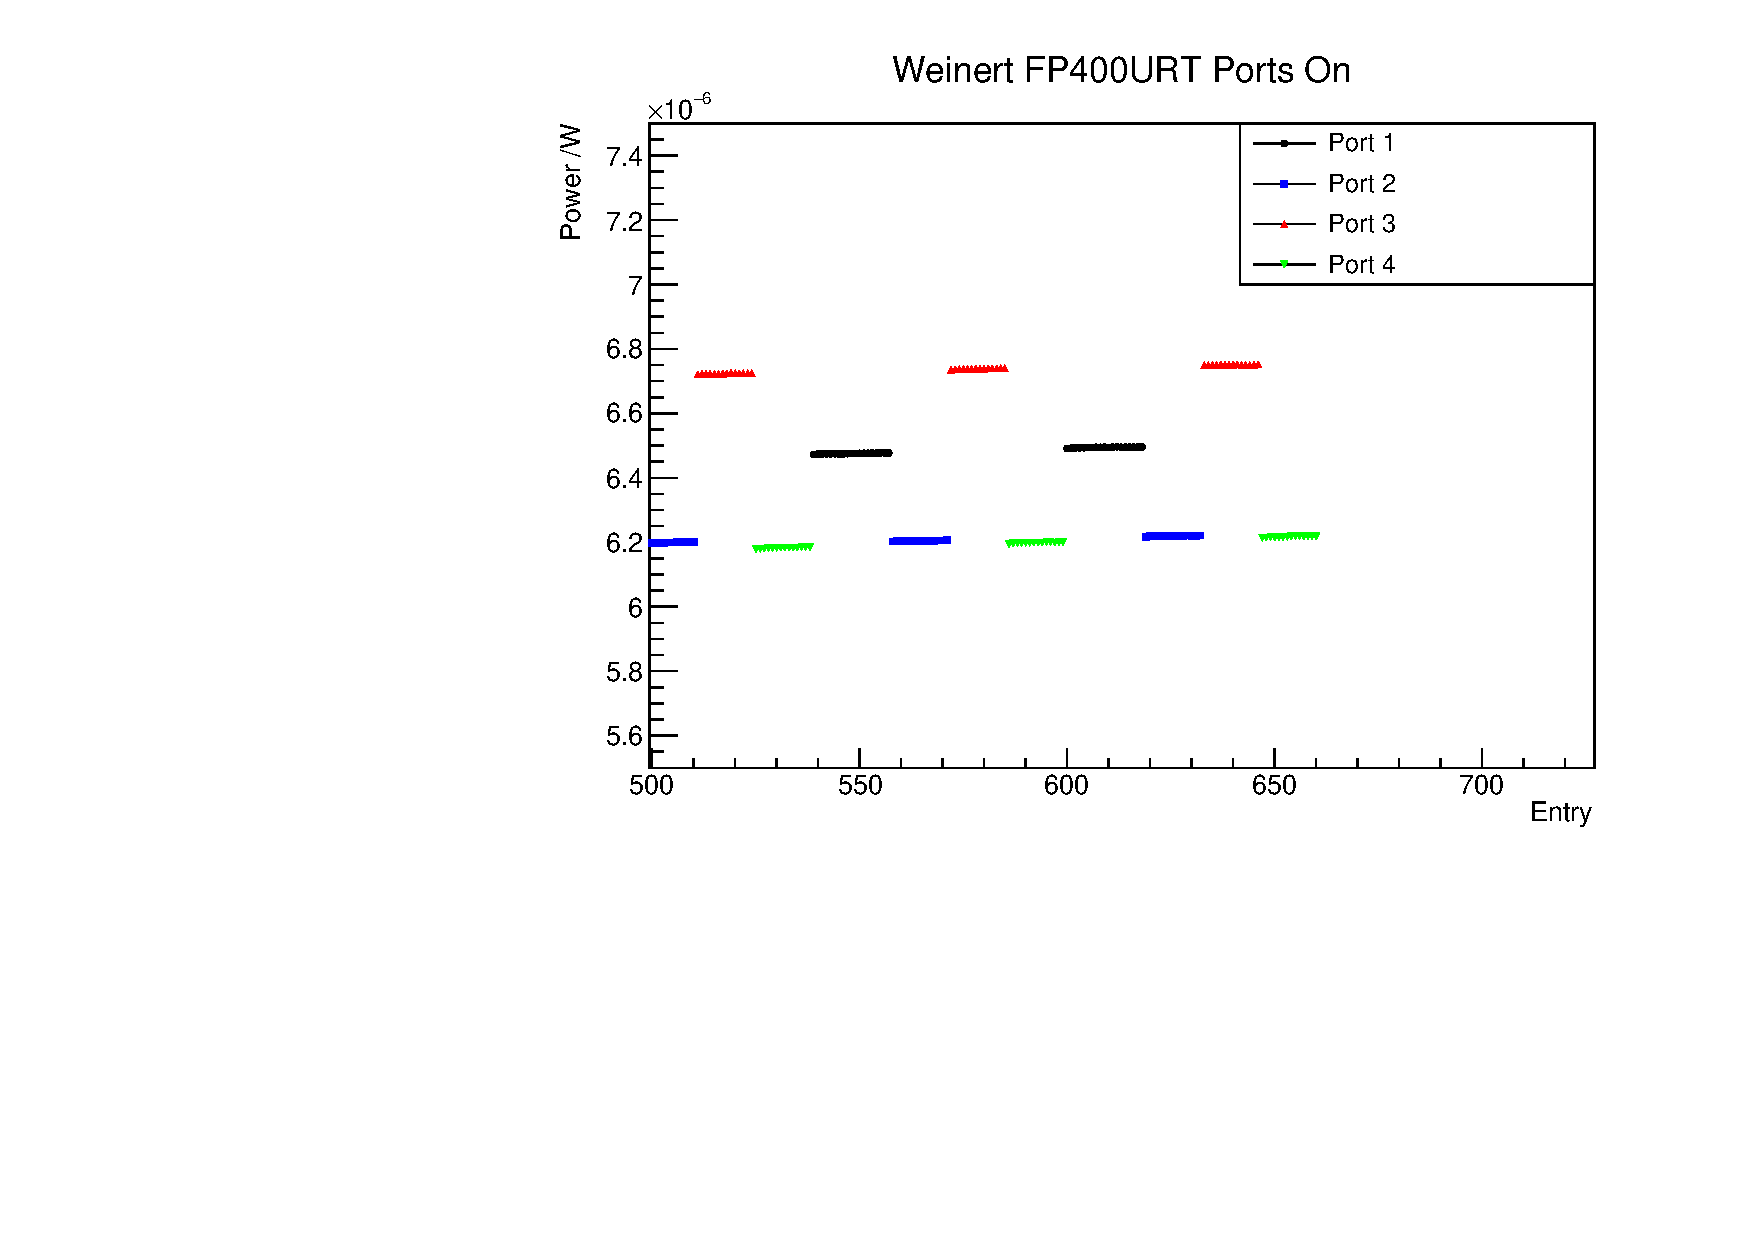
\includegraphics[width=\linewidth]{WeinertFP400URTPortsOnZoom.pdf}
\subcaption{}\label{fig:weinfp400crosstalkon}
\end{subfigure}%
\begin{subfigure}{0.5\textwidth}
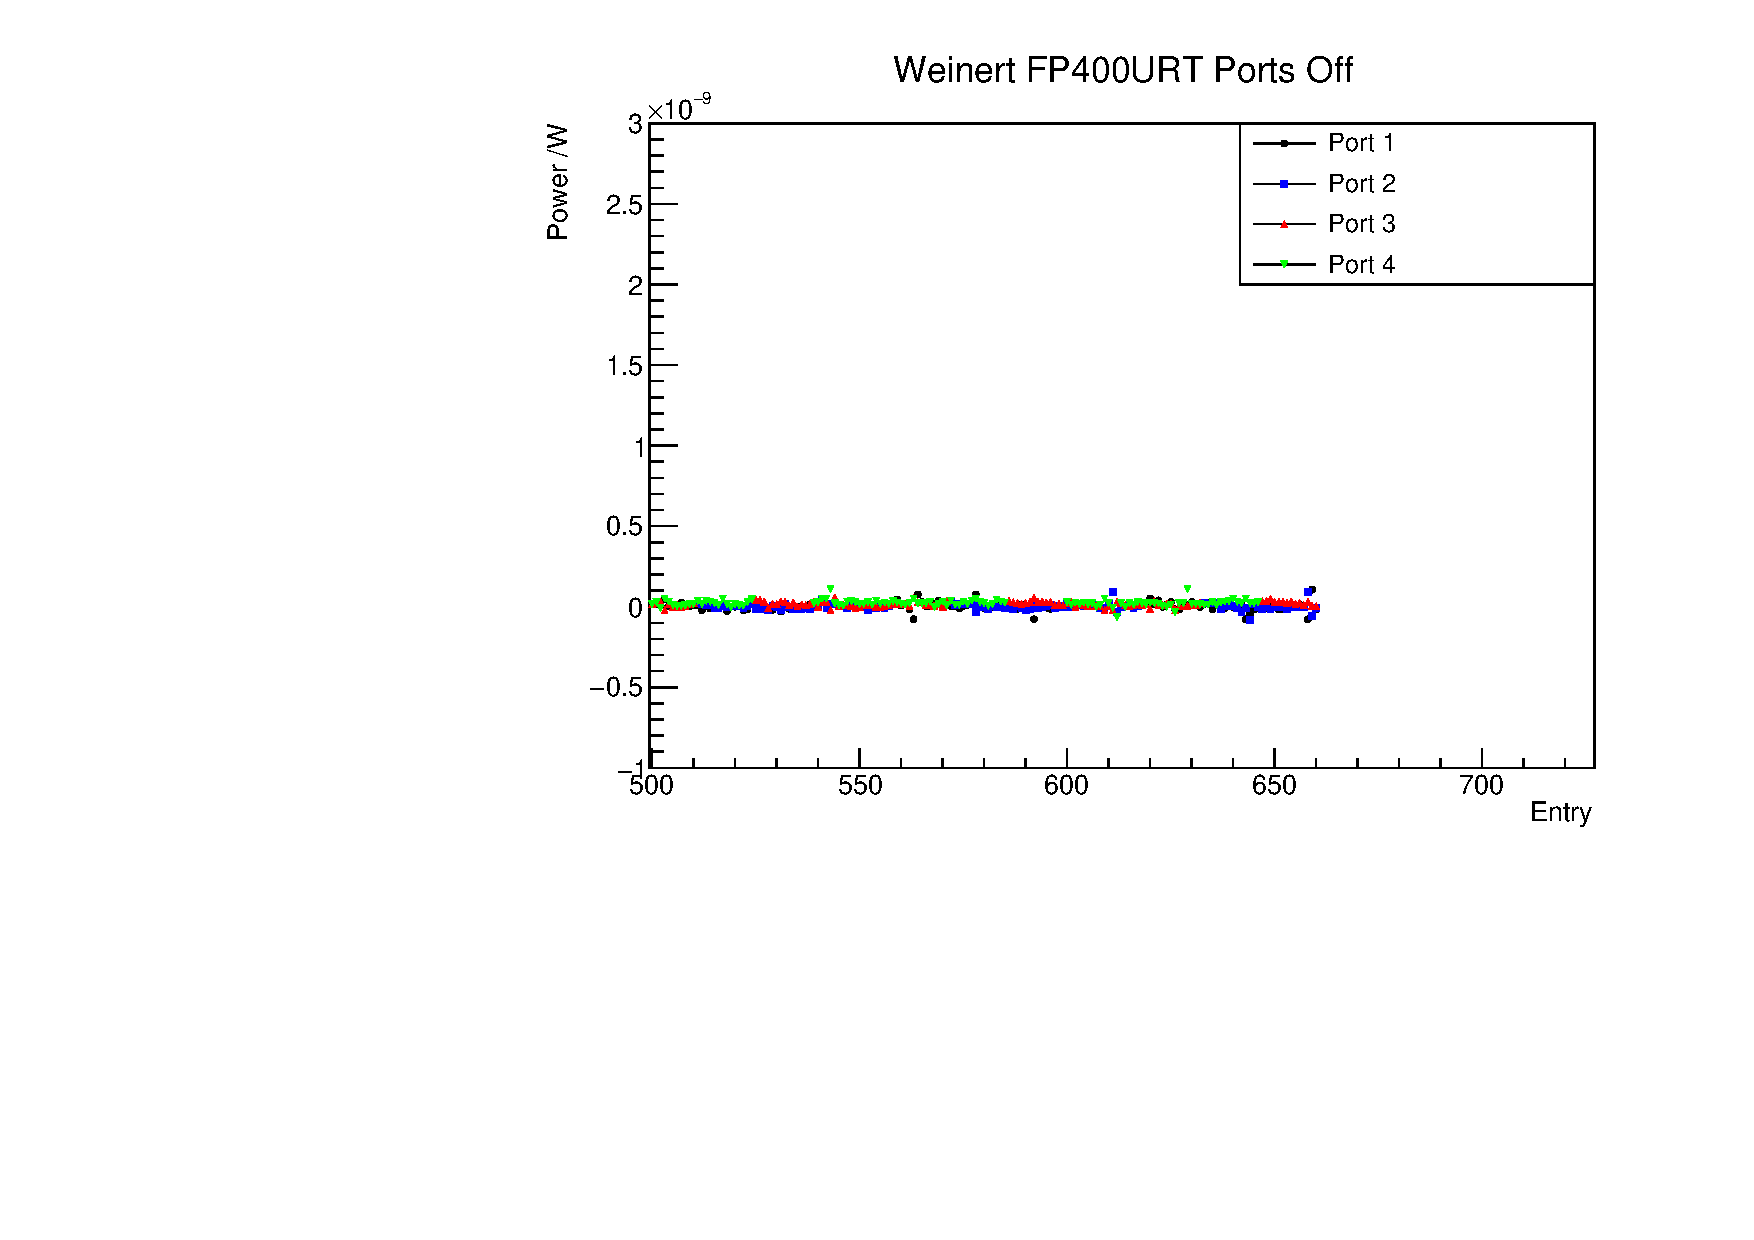
\includegraphics[width=\linewidth]{WeinertFP400URTPortsOffZoom.pdf}
\subcaption{}\label{fig:weinfp400crosstalkoff}
\end{subfigure}
\caption{Power meter readings from all four ports for the Weinert FP400URT device, zoomed into a shorter period of data to better show structure. Data is shown for when ports are a) illuminated and b) not illuminated. Note the different y-axis scales.}\label{fig:weinfp400crosstalk}
\end{figure}
\begin{figure}[h!]
\centering
\begin{subfigure}{0.5\textwidth}
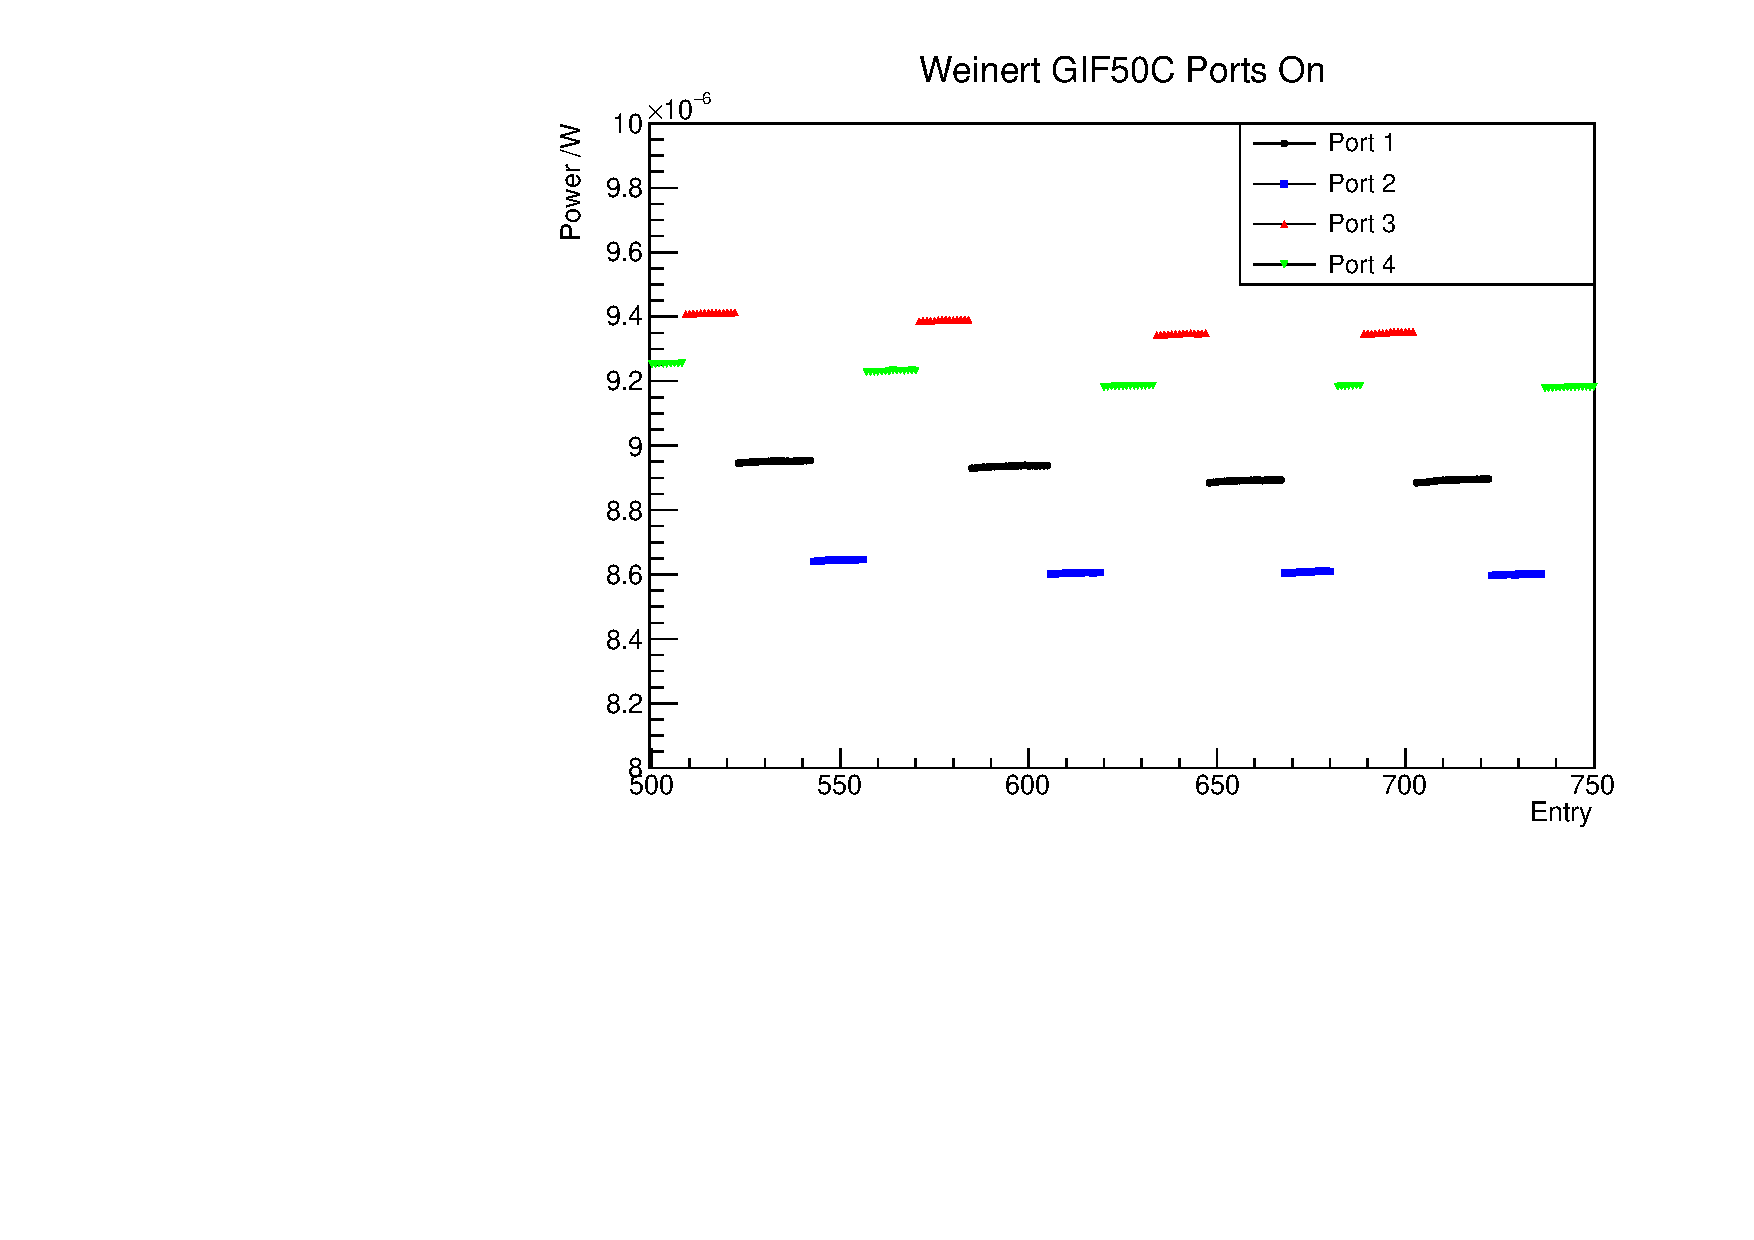
\includegraphics[width=\linewidth]{WeinertGIF50CPortsOnZoom.pdf}
\subcaption{}\label{fig:weingifcrosstalkon}
\end{subfigure}%
\begin{subfigure}{0.5\textwidth}
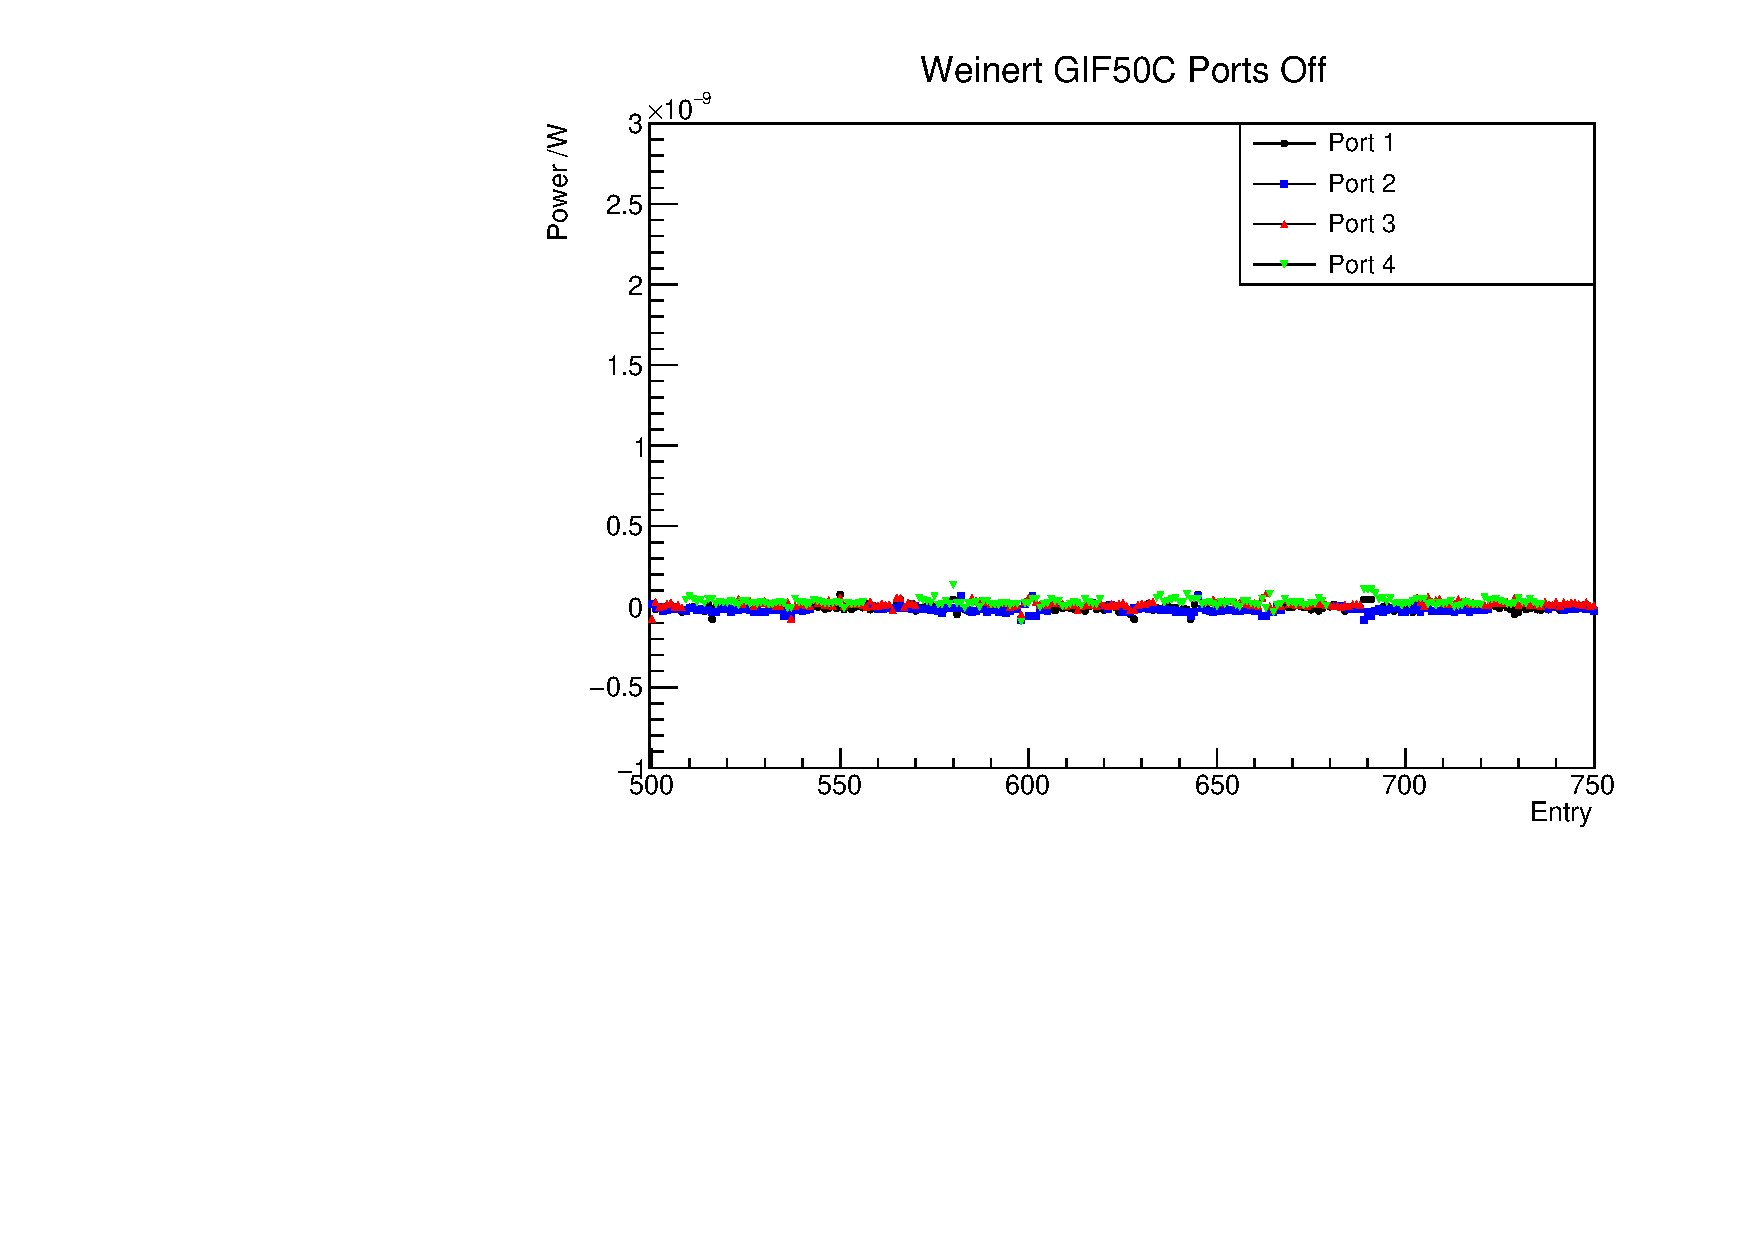
\includegraphics[width=\linewidth]{WeinertGIF50CPortsOffZoom.pdf}
\subcaption{}\label{fig:weingifcrosstalkoff}
\end{subfigure}
\caption{Power meter readings from all four ports for the Weinert GIF50C device, zoomed into a shorter period of data to better show structure. Data is shown for when ports are a) illuminated and b) not illuminated. Note the different y-axis scales.}\label{fig:weingifcrosstalk}
\end{figure}
The most interesting result is seen in \cref{fig:agifp400crosstalkoff}, which shows clear changes in the power readings recorded on ports 1 and 2, when these ports are not illuminated. There is also a repeating structure to the data from port 4 suggesting a lower level of crosstalk to that channel. This suggests varying levels of crosstalk between different ports. \cref{fig:weinfp400crosstalkoff,fig:weingifcrosstalkoff} on the other hand show no measurable cross talk between any of the channels.

To further investigate this, the way the data is plotted was inverted. The four plots in \cref{fig:agifp400crosstalk2} show the power recorded on a specific port, each separated by which of the other three ports was illuminated at the time.
\begin{figure}[h!]
\centering
\begin{subfigure}{0.5\textwidth}
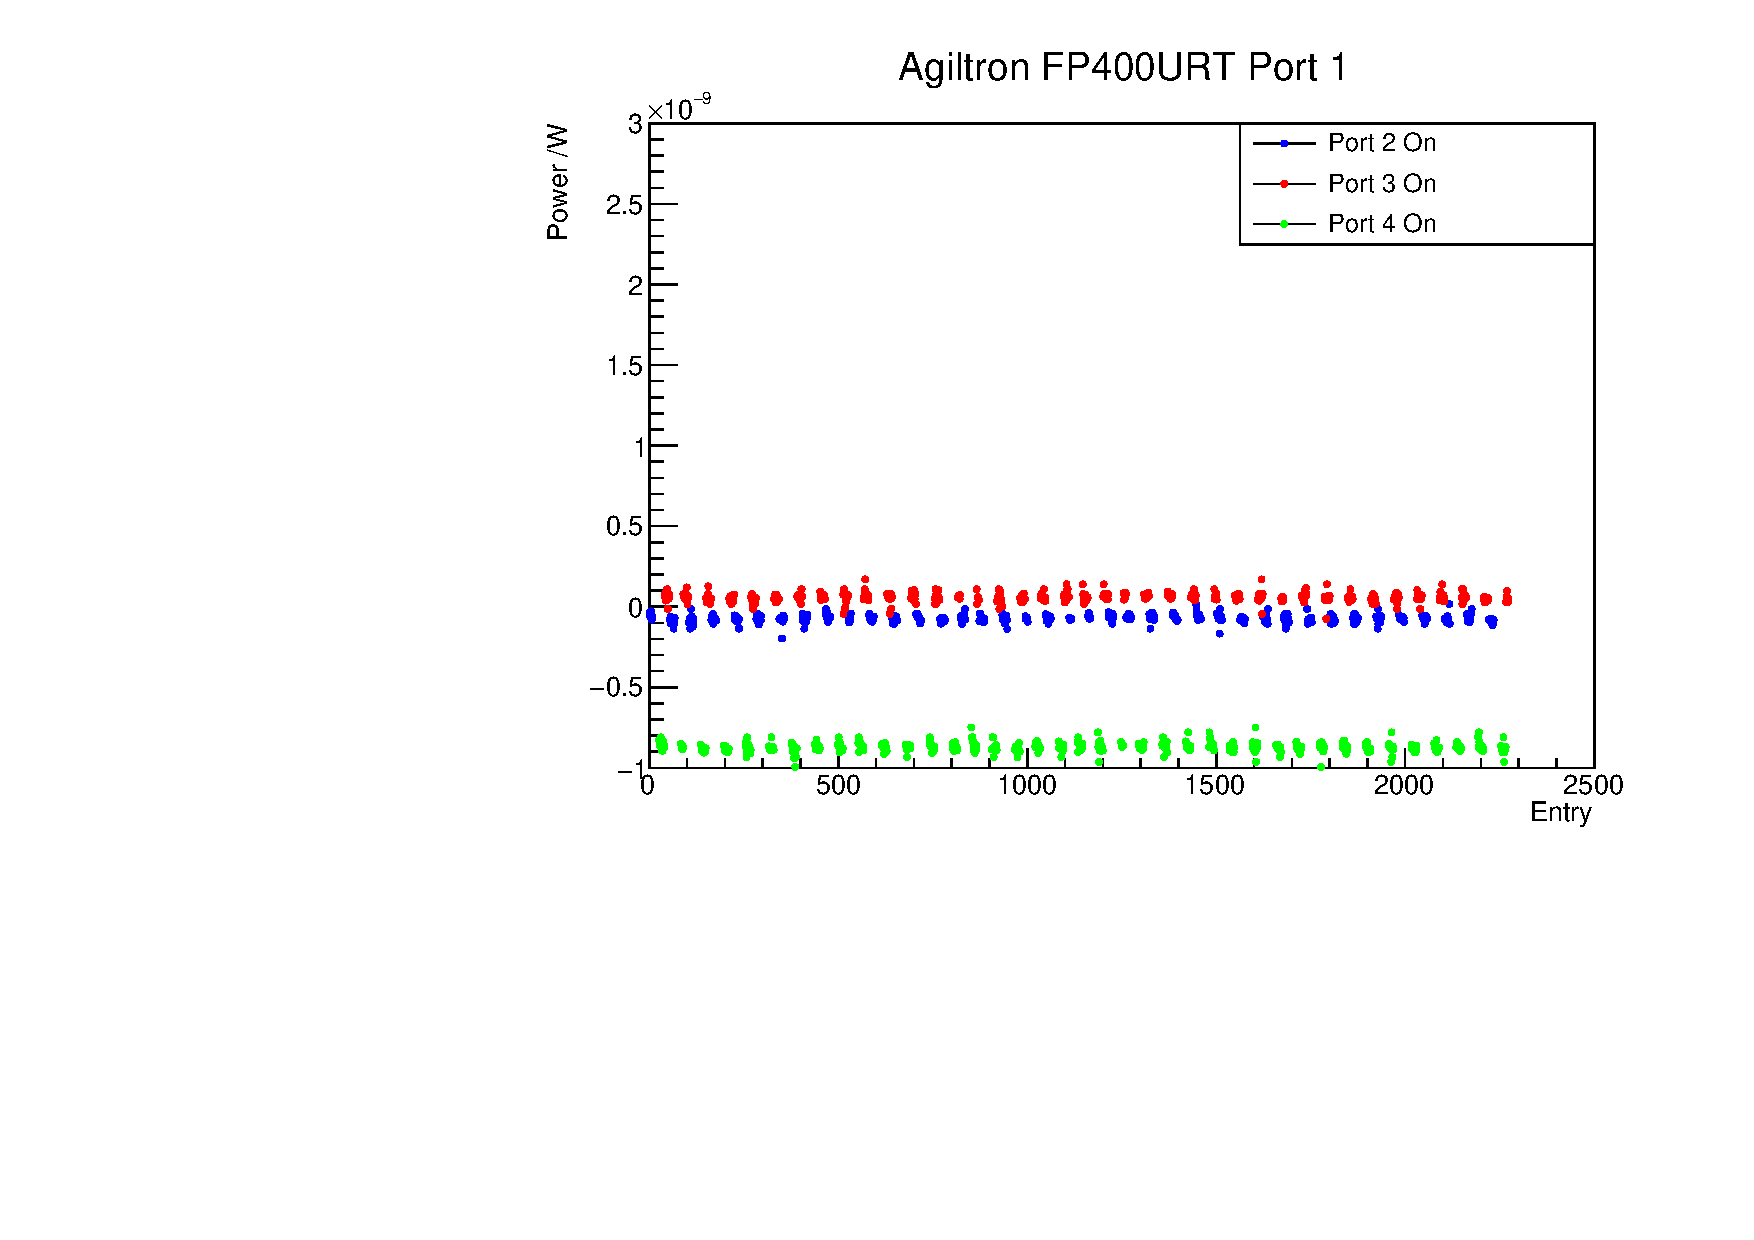
\includegraphics[width=\linewidth]{AgiltronFP400URTPort1.pdf}
\subcaption{}\label{fig:agifp400crosstalkport1}
\end{subfigure}%
\begin{subfigure}{0.5\textwidth}
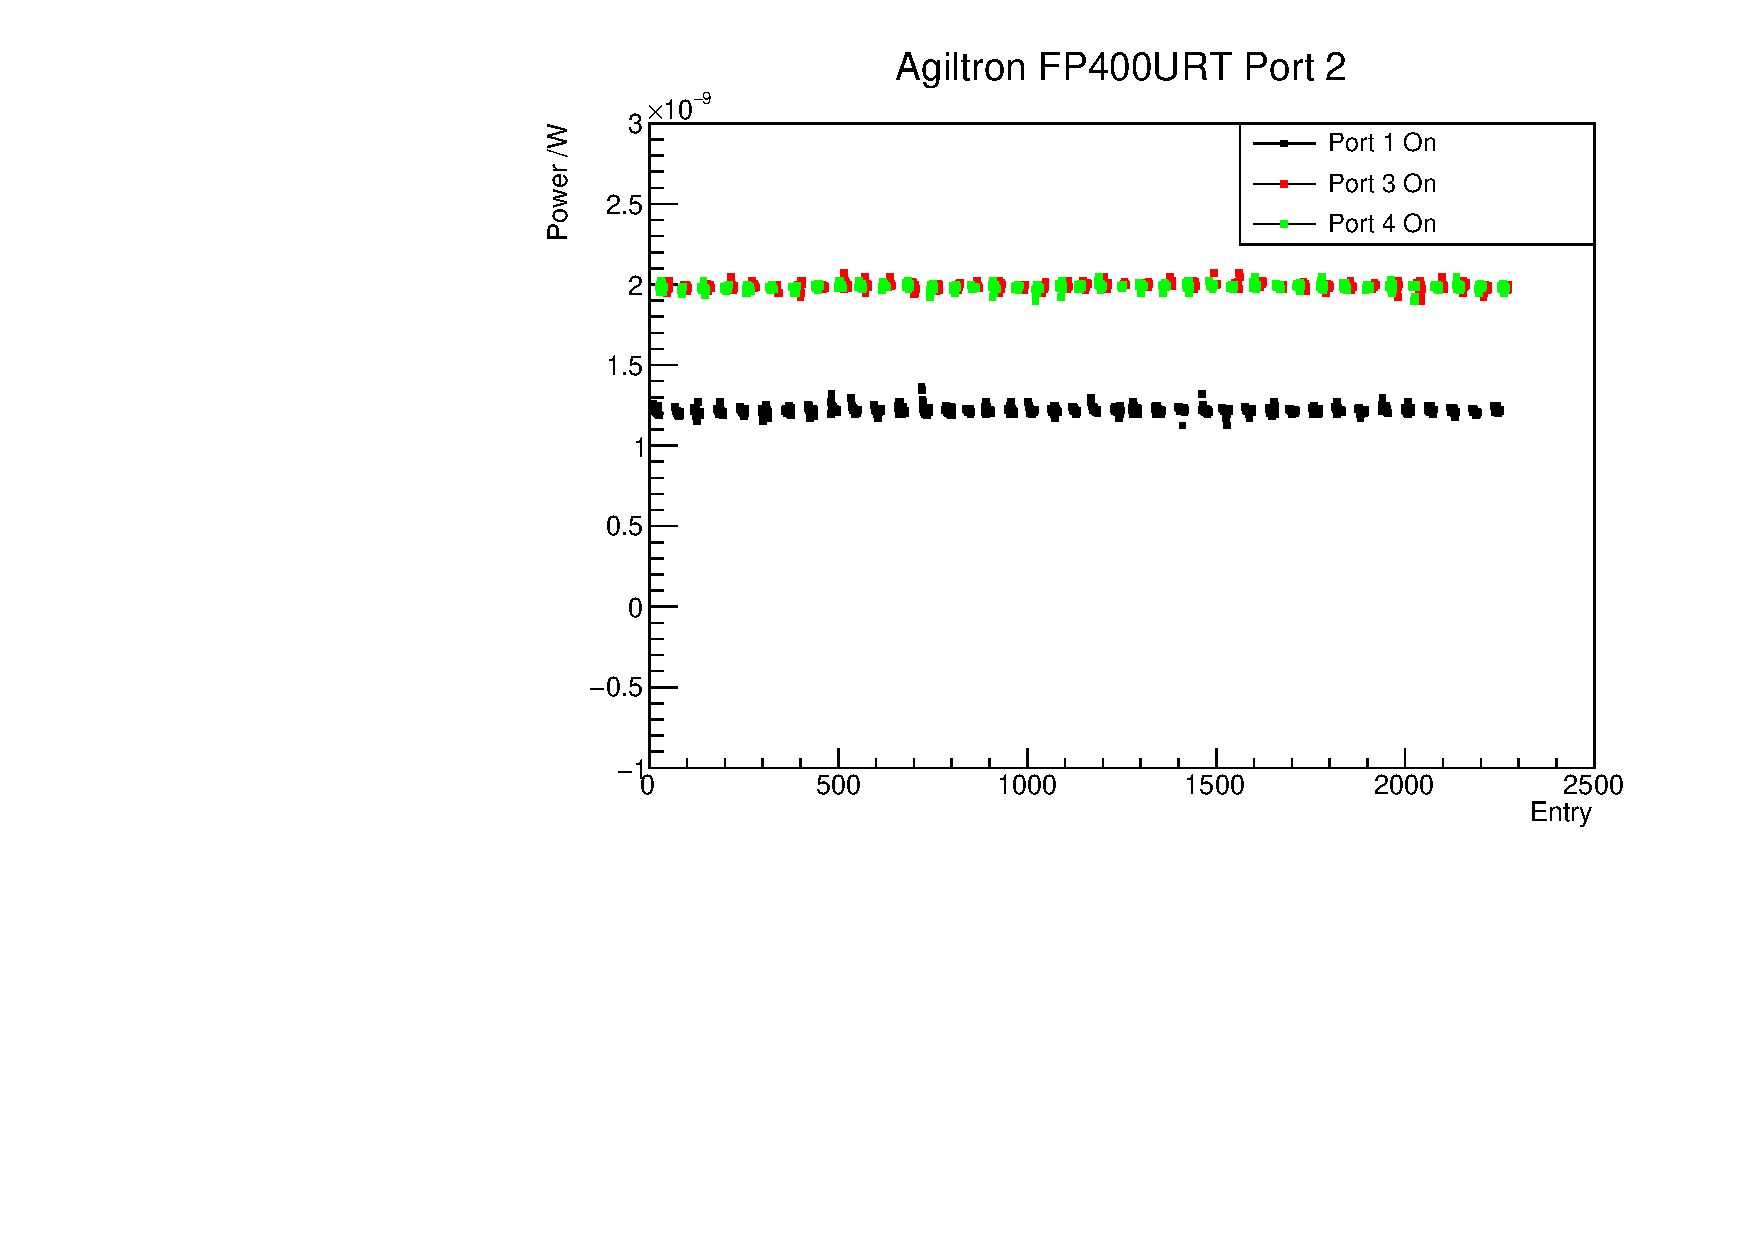
\includegraphics[width=\linewidth]{AgiltronFP400URTPort2.pdf}
\subcaption{}\label{fig:agifp400crosstalkport2}
\end{subfigure}
\\
\begin{subfigure}{0.5\textwidth}
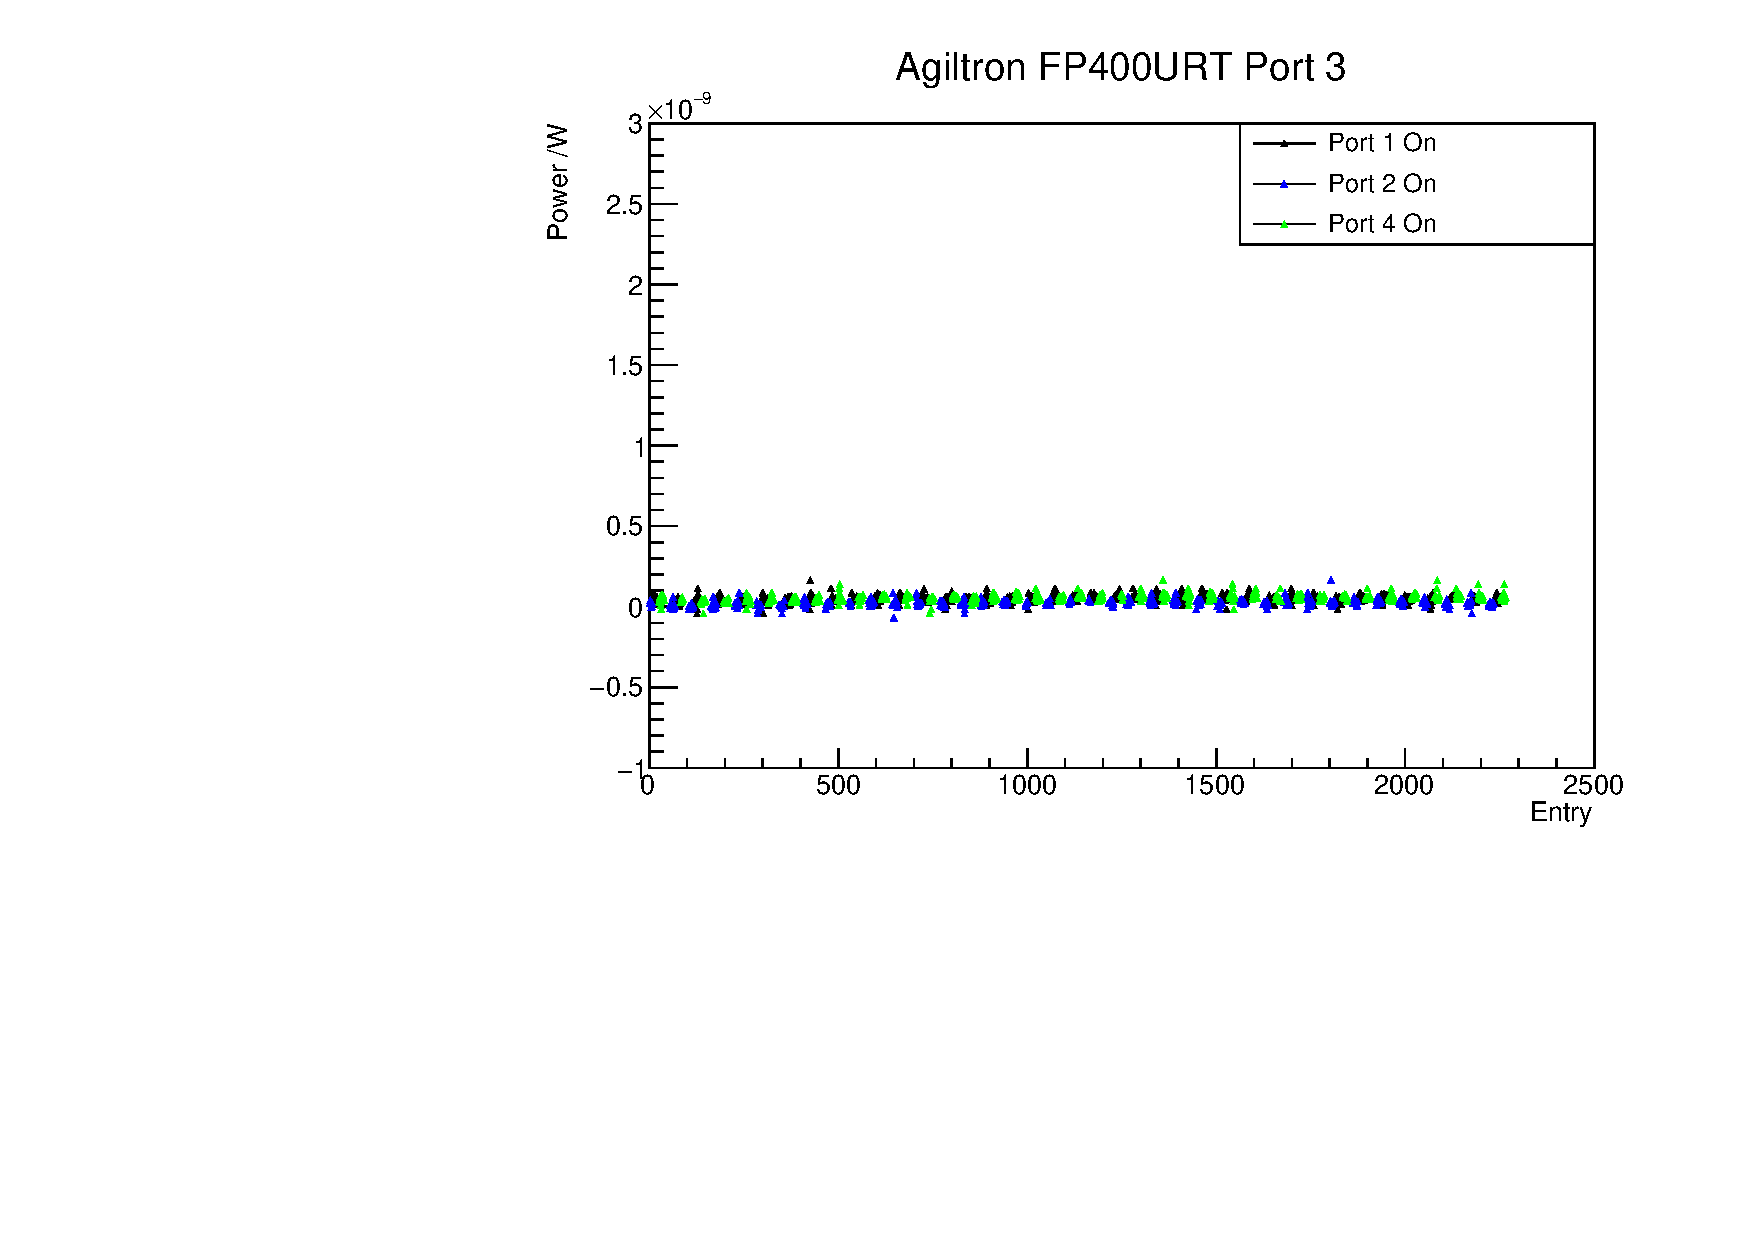
\includegraphics[width=\linewidth]{AgiltronFP400URTPort3.pdf}
\subcaption{}\label{fig:agifp400crosstalkport3}
\end{subfigure}%
\begin{subfigure}{0.5\textwidth}
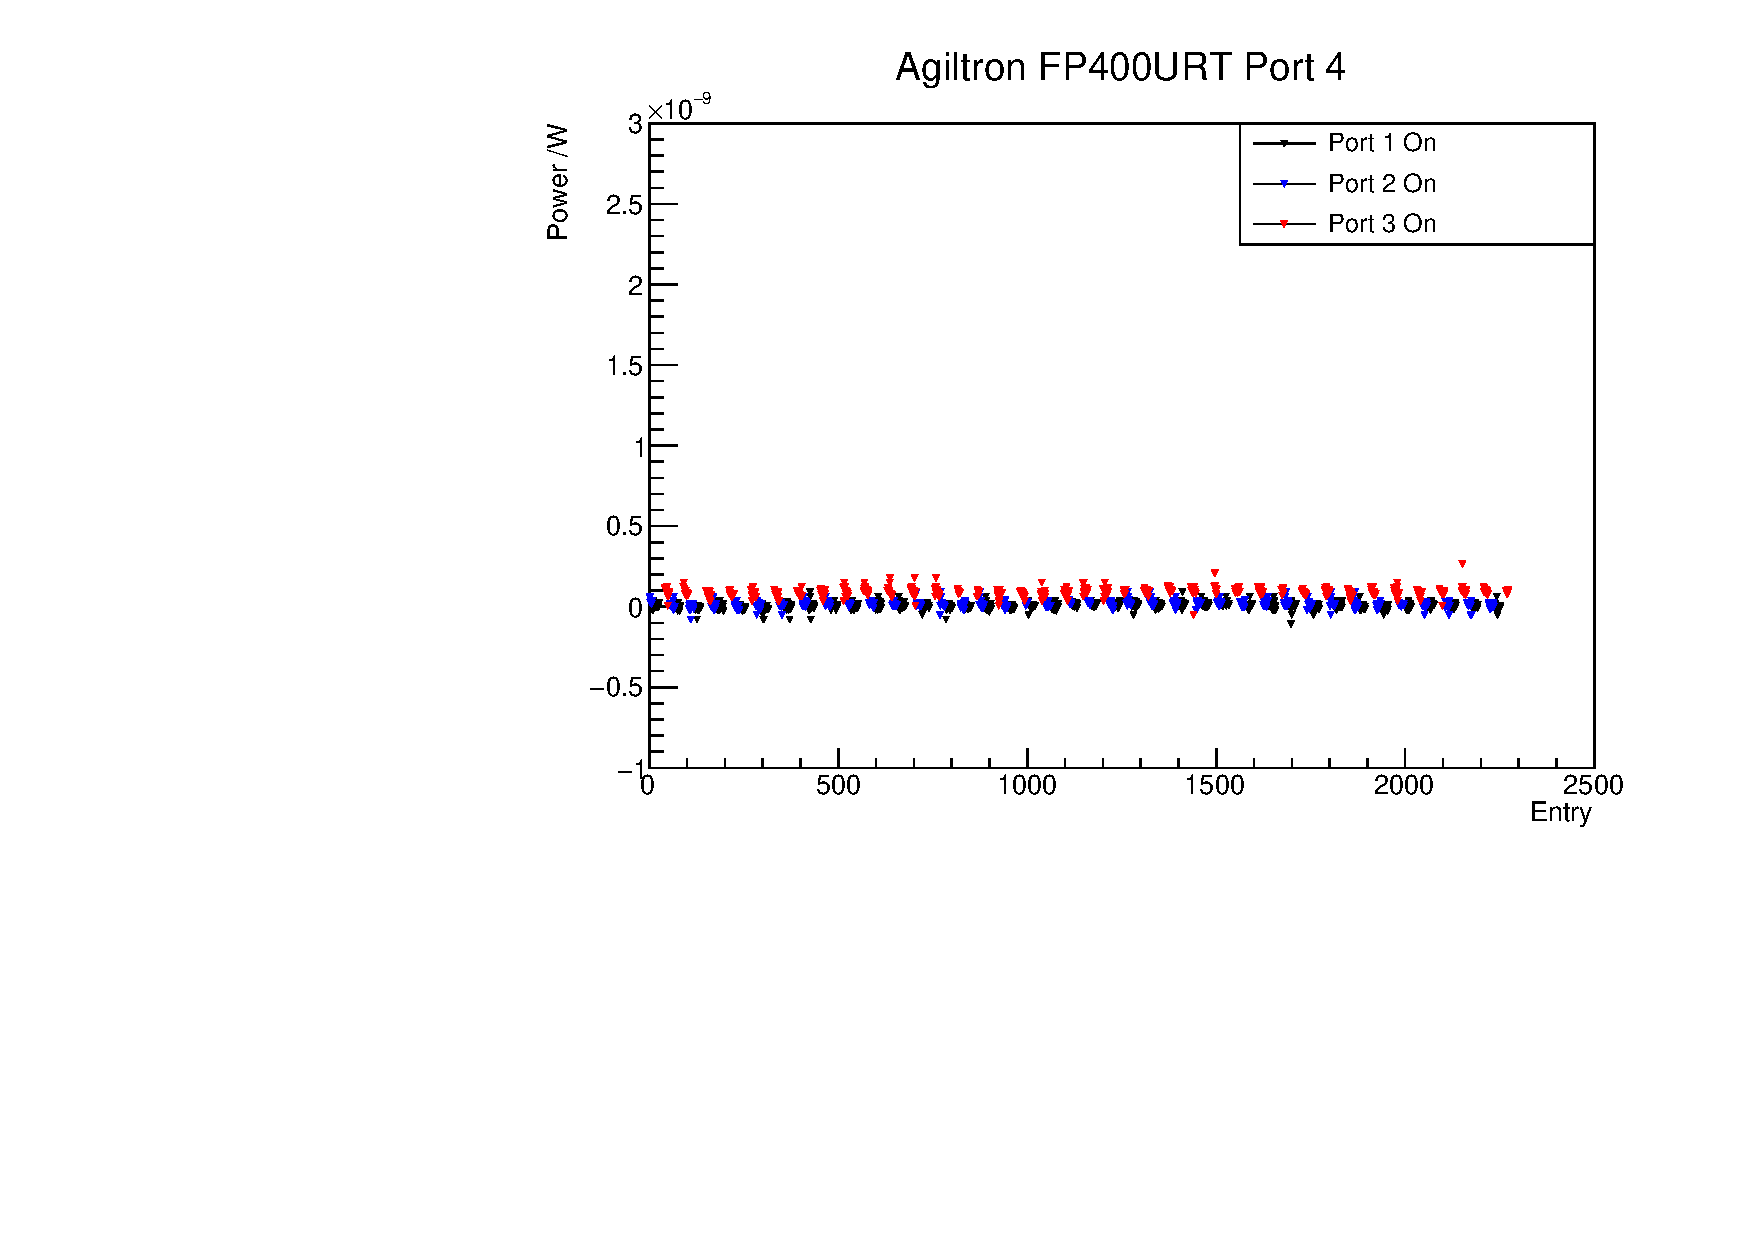
\includegraphics[width=\linewidth]{AgiltronFP400URTPort4.pdf}
\subcaption{}\label{fig:agifp400crosstalkport4}
\end{subfigure}
\caption{Power recorded on a) port 1, b) port 2, c) port 3 and d) port 4 of the Agiltron FP400URT switch, when one of the other three ports was illuminated.}\label{fig:agifp400crosstalk2}
\end{figure}
While the absolute value of the power is not expected to be exactly zero due to global drift caused by temperature changes in the lab over the course of data taking, all four power meters were calibrated at the same time, so should show the same level of power when not illuminated. This is clearly not the case for ports 1 and 2 (\cref{fig:agifp400crosstalkport1,fig:agifp400crosstalkport2}), with the former showing higher power readings when port 2 or port 3 were illuminated, and the latter showing the same when port 3 or port 4 were illuminated. There is also a small offset observed for port 4 in \cref{fig:agifp400crosstalkport4}, when port 3 is being illuminated. Interestingly, no obvious cross talk was observed to port 3, from any of the other ports being illuminated.

As no cross talk was observed for either of the Weinert devices, the corresponding plots are not shown here, but are given in \cref{fig:weinfp400crosstalk2,fig:weingifcrosstalk2} in \cref{app:crosstalk} for completeness.

\subsection{Summary}
Testing of the three different fibre switching devices finds different devices come out best based on different factors. The Weinert GIF50C device showed best power transmission, with at most 4.7\% loss compared to the reference fibre, while the Weinert FP400URT device showed up to 27.6\% loss. This is with the caveat that the device package was different, and the latter had a greater length of fibre than both the other devices and the reference fibre used. All devices exhibited under 5\% variation in output power across the four ports, with the Agiltron switch showing the least variation at a difference of 2.61\%.

A clear preference for the Weinert devices comes from the cross talk measurements, which show measurable cross talk between certain channels on the Agiltron device. While this is at the level of $\mathcal{O}(0.1\%)$, the lack of any measurable cross talk from either of the Weinert devices is clearly preferable. Coupled with the superior support from Weinert which will make setup and potential servicing of the hardware easier, this is the device that is preferred. The internal fibre will of course be chosen to match what is used for the rest of the laser system, so will be Thorlabs FG105UCA or equivalent.


\section{Speed of Light Measurements}\label{sec:c}

As will be discussed in further detail in \cref{sec:lengths}, the lengths of fibre optic cables connecting to the injectors will not be uniform. This presents additional challenges for the system as different path lengths result in different levels of attenuation and dispersion and, in particular, offsets in delays between signals in the electronics and actual light injection into the tank. For example, the injection event using a diffuser on the end of a $\sim160$~m fibre will occur much later than when the input light has to only traverse 10~m of fibre. To account for this, delays should be incorporated into the electronics based on the expected time taken for a light pulse to be injected. To this end, the speed of light within the FG105UCA fibre was measured, to understand if this offset could be easily implemented.

Using the fibre test stand with the laser setup, the relative time delay between the laser trigger signal and the PMT signal was recorded, for fibre lengths of 1~m, 35~m, 107~m and 142~m. As with previous measurements, due to the fragility of the untubed 105~m reel of FP400URT, 1~m patch fibres were used to connect it into the system. Time delay values were recorded at each length for 20,000 events, in order to obtain uncertainties. The results for this are shown in \cref{fig:FP400URTc}, where the data is fit with a linear function to calculate the necessary time delay in the electronics per metre of fibre.
\begin{figure}[h]
\centering
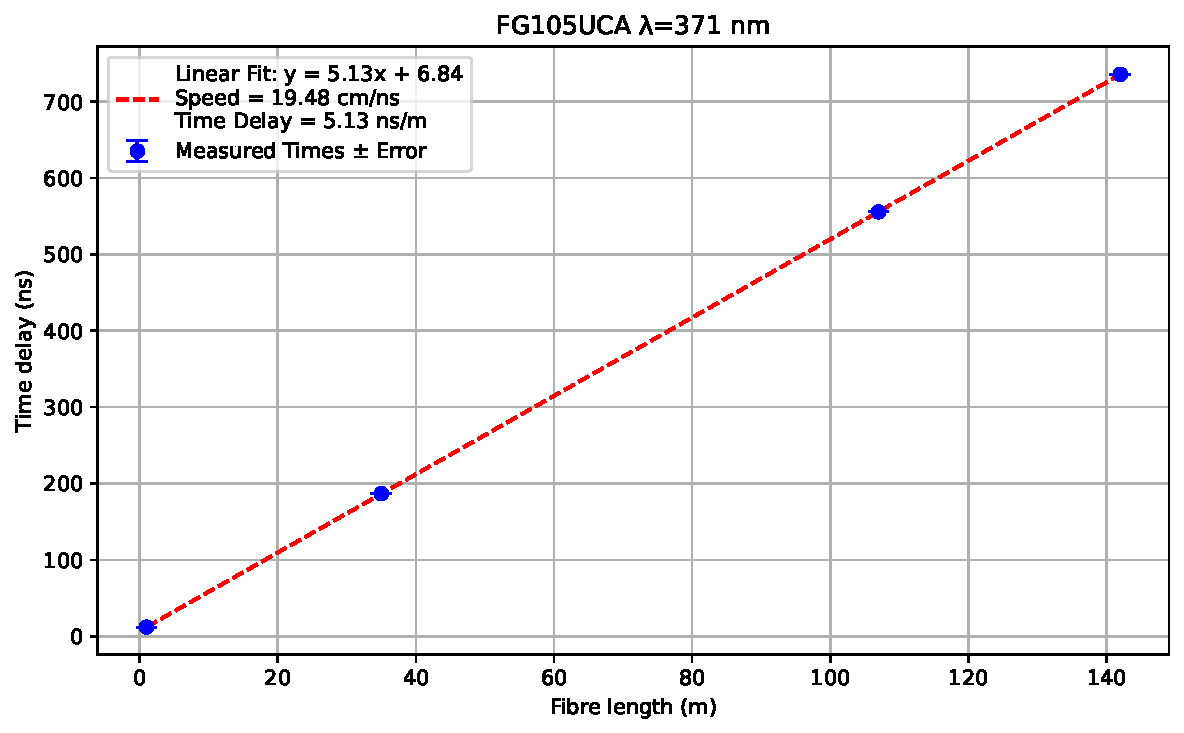
\includegraphics[width=0.8\textwidth]{FG105UCATiming_371nm.pdf}
\caption{Time delay measurements from the FG105UCA fibres using the 371~nm laser head.}\label{fig:FP400URTc}
\end{figure}
This verifies that the speed of light can easily be measured with this setup, and that including connectors has no obvious impact on the expected results. Naturally, as the speed of light in any medium is wavelength dependent, this will need calculating for every wavelength of light used in the LI system.

\DIFaddbegin \section{\DIFadd{Destructive Testing}}\label{sec:destruction}
\DIFadd{Another important aspect of the fibres to test is their durability. While every care should be taken with the fibres to ensure damage does not occur, they will be installed in a working environment, and accidents can happen.  With a large number of fibres of varying length, visually noticing damage to a fibre is very unlikely. As such, it is important to understand what kinds of stress a fibre can realistically be exposed to and what can be tolerated, along with how to quickly check if damage has occurred.
}

\DIFadd{As these tests need to be carried out in a working environment, using the same set-up as in the fibre optic test stand (\mbox{%DIFAUXCMD
\cref{sec:meas:sub:stand}}\hskip0pt%DIFAUXCMD
) is not viable. Instead, commercially available, hand-held testing devices were investigated, and three units of the TREND Networks FiberMASTER MM testing kit \mbox{%DIFAUXCMD
\cite{bib:TREND} }\hskip0pt%DIFAUXCMD
were purchased. This is a hand-held, battery operated light source and power meter, with varied wavelengths between 850--1550~nm. Although this is not the operating wavelength of the LI system, it still allows for quick checks of through-put power, and any damage to the fibres will still be obvious in changed readings.
}

\DIFadd{A series of tests were carried out to assess the resilience of FP400URT and FG105UCA 1~m patch fibres to crushing, bending and cutting, plus scraping of the connector ends. The results for these are briefly summarised here. }{\bf \DIFadd{can go into more detail if desired, but Unik has a lot of info that needs condensing into this section}}

\subsection{\DIFadd{Crushing}}
\DIFadd{The first set of tests carried out consisted of applying a series of increased weights to the fibres. This started with simply applying bodyweight (\mbox{%DIFAUXCMD
$\sim80$
}%DIFAUXCMD
~kg) through stepping on the fibres, the most likely scenario for them to experience stress. No visible damage or change in power output was observed in this case.
}

\DIFadd{To increase the force experienced, a trolley was used to apply a series of weights from 100--160~kg through a single wheel. At the maximum weight of 160~kg, a 24\% reduction in output power was observed, but this returned to normal once the weight was removed. Visual inspection of the fibre revealed some yellowing caused by stress to the fibre, but no other signs of permanent damage were observed. To push this further, the fibre was then driven over by a small car (\mbox{%DIFAUXCMD
$sim$
}%DIFAUXCMD
330~kg per wheel), while connected to the hand-held test kit. Static compression was seen to reduce the power output by 60\%, but again only while the weight remained on the fibre, returning back to nominal after being removed. As a final test, the fibre was also exposed to shearing forces, by turning the car's wheels whilst stationary on the fibre. This caused a sharp drop in power of 86\% and clear structural damage, as the power output did not recover after removing the weight.
}

\subsection{\DIFadd{Bending}}
\DIFadd{These tests explored how the fibres responded to manual bending and twisting, particularly beyond the specified bending radius. Fibres were observed to tolerate mild bends without degradation, however when forming angles below 90}\degree\DIFadd{\ significant signs of degradation occurred, particularly if bent in locations of previous wear. For the FG105UCA, a sharp bend in its midpoint caused a power reduction of 35--55\%, and ultimately breakage when folded back on itself. Results were similar with the FP400URT. Though only exploratory, these tests highlighted the importance of maintaining the quoted bending radius and the care that should be taken when deploying fibres.
}

\subsection{\DIFadd{Cutting}}
\DIFadd{This test was to evaluate the physical resilience of the furcation tubing when exposed to sharp tools. In these tests, a utility knife, pliers and scissors were used. The utility knife was unable to penetrate the tubing with multiple passes, however the pliers and scissors were able to cut through the whole fibre with moderate effort. This suggests that the furcation tubing is capable of holding up to passing cuts, but not when blades are applied with reasonable force. Care should be taken when working with any sharp object around fibres, and any exposure minimised.
}

\subsection{\DIFadd{Scraping}}
\DIFadd{This test focussed completely on the fibre connectors, applying surface abrasion to simulate damage caused by the connectors being dragged along floors or scraped against surfaces during installation. \mbox{%DIFAUXCMD
\cref{fig:scraping} }\hskip0pt%DIFAUXCMD
shows microscope images taken of the connectors, where the extent of the damage to the internal fibre core after scraping along the lab floor can easily be seen.
}\begin{figure}[h]
\centering
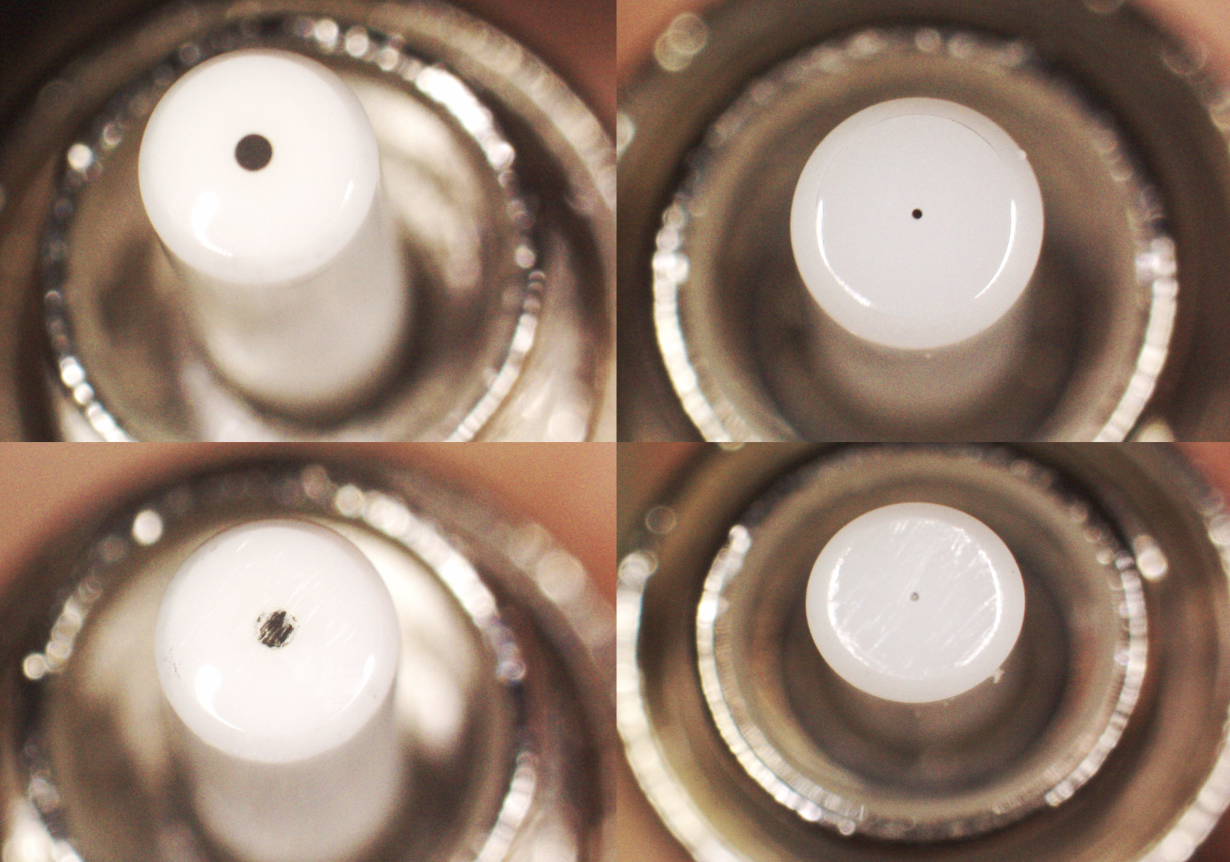
\includegraphics[width=0.7\textwidth]{scraping}
\caption{\DIFaddFL{Microscope images of connectors for FP400URT (left) and FG105UCA (right) before (top) and after (bottom) scraping along the lab floor.}}\label{fig:scraping}
\end{figure}
\DIFadd{A permanent reduction in power of up to 50\% was observed after causing this damage. This highlights the need to keep all ends of fibres protected by dust caps throughout shipping, testing and installation, right up until the point of connection.
}


\section{\DIFadd{Reception Testing}}\label{sec:testing}
\DIFadd{\mbox{%DIFAUXCMD
\cref{sec:lengths} }\hskip0pt%DIFAUXCMD
will discuss the number of fibres required for the entire LI system to be built. In an ideal scenario, all fibres will be delivered to Japan with no issues. However, with such a large order, the potential for small defects in manufacturing or some damage in shipping must be accounted for. A contingency of \mbox{%DIFAUXCMD
$\sim$
}%DIFAUXCMD
10\% will be assumed in quotes to account for this. Upon receipt of the fibres in Japan, several tests should be carried out to ensure the fibres are performing as expected.
}

\DIFadd{With nearly 1000 fibres in total, full characterisation of each one is not viable. Instead, upon delivery of each set of fibres, quick checks of power output through each fibre will be performed with the hand-held testing device detailed in \mbox{%DIFAUXCMD
\cref{sec:destruction}}\hskip0pt%DIFAUXCMD
. By measuring the transmitted power through all fibres in a set a distribution of values can be built, and the largest outliers excluded down to the number of required fibres. Specification sheets for the FG105UCA \mbox{%DIFAUXCMD
\cite{bib:fg105uca} }\hskip0pt%DIFAUXCMD
and FP400URT \mbox{%DIFAUXCMD
\cite{bib:fp400urt} }\hskip0pt%DIFAUXCMD
provide measured attenuation values for a range of wavelengths. By comparing the batch average power to the expectation when accounting for attenuation, any difference should be immediately obvious, and significant issues would be raised with the supplier straight away. During installation of the fibres, power readings with the hand-held devices will be repeated, to ensure no damage has occurred to fibres in the process.
}

\DIFadd{While it will not be possible to extensively test all fibres, more detailed batch testing of fibres upon delivery to Japan is required. This will be carried out using a very similar set-up to the Liverpool fibre optic test stand (described in \mbox{%DIFAUXCMD
\cref{sec:meas:sub:stand}}\hskip0pt%DIFAUXCMD
), which will be reproduced in the lab space in Japan, using the laser system which will then be installed as a light source for the ID injectors. Arguably the most important measurements to be made here will be those of the speed of light in fibres. These will be carried out following the same prescription as in \mbox{%DIFAUXCMD
\cref{sec:c}}\hskip0pt%DIFAUXCMD
, for both fibre types. As the speed of light in a medium is wavelength-dependent, this will be done for every appropriate wavelength, with the measurements being used to define the required offsets in electronics to account for different lengths of fibres used. In addition to speed of light measurements, batch testing of attenuation and pulse widths will be carried out to screen for potential issues.
}


\DIFaddend \section{Fibre Length Requirements}\label{sec:lengths}

With the large number of injectors being employed for the light injection system, an even larger number of fibre optic cables will be required. This section details the quantity and lengths of cables required to connect the full HK LI system.

The overall design of the HK water tank and PMT support structure is given in \cref{fig:HKtank}. Fibre optics will run through specifically installed fibre ports around the edge of the dome floor into the OD, then down to each injector location.
\begin{figure}[h]
\centering
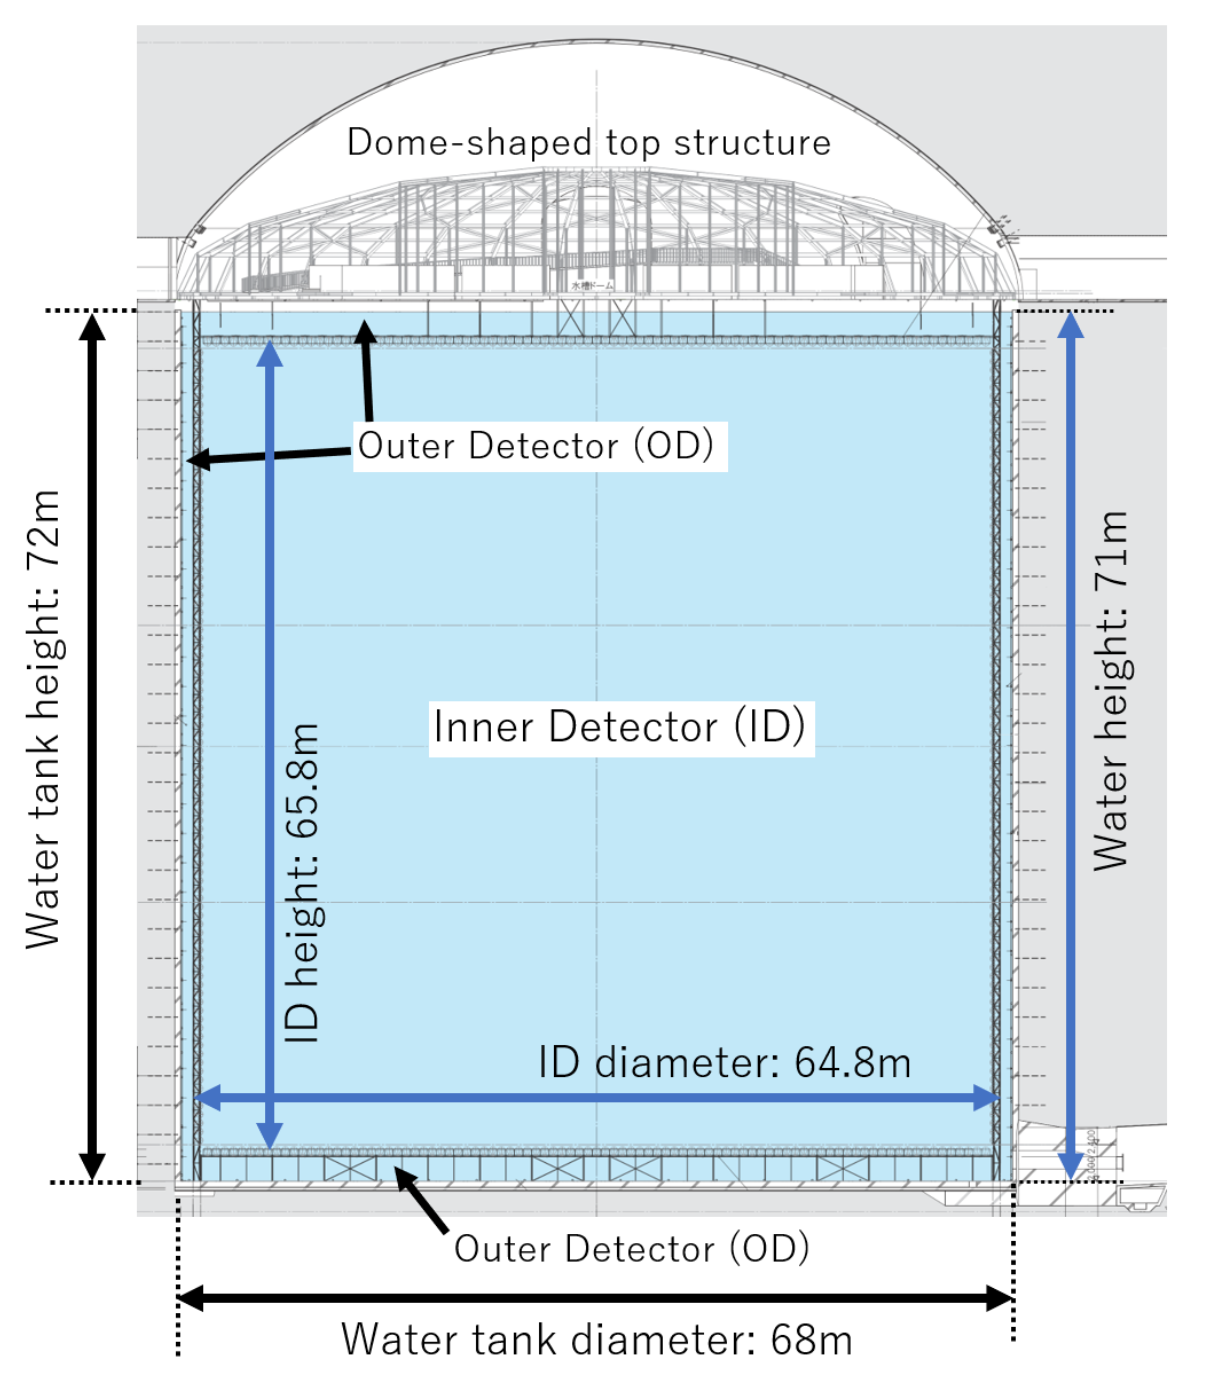
\includegraphics[width=0.6\textwidth]{HKdiagram.png}
\caption{Schematic of the HK water tank and PMT support structure. \cite{bib:tn0048}}\label{fig:HKtank}
\end{figure}
16 of these fibre ports are distributed roughly evenly around the outer edge of the dome. The full schematic of the dome showing all calibration and fibre ports is given in \cref{fig:ports}. The OD fibre ports in question are those marked with magenta dots and labelled ``odf'' (OD(\begin{CJK*}{UTF8}{min}ファイバー用\end{CJK*})).
\begin{figure}[h]
\centering
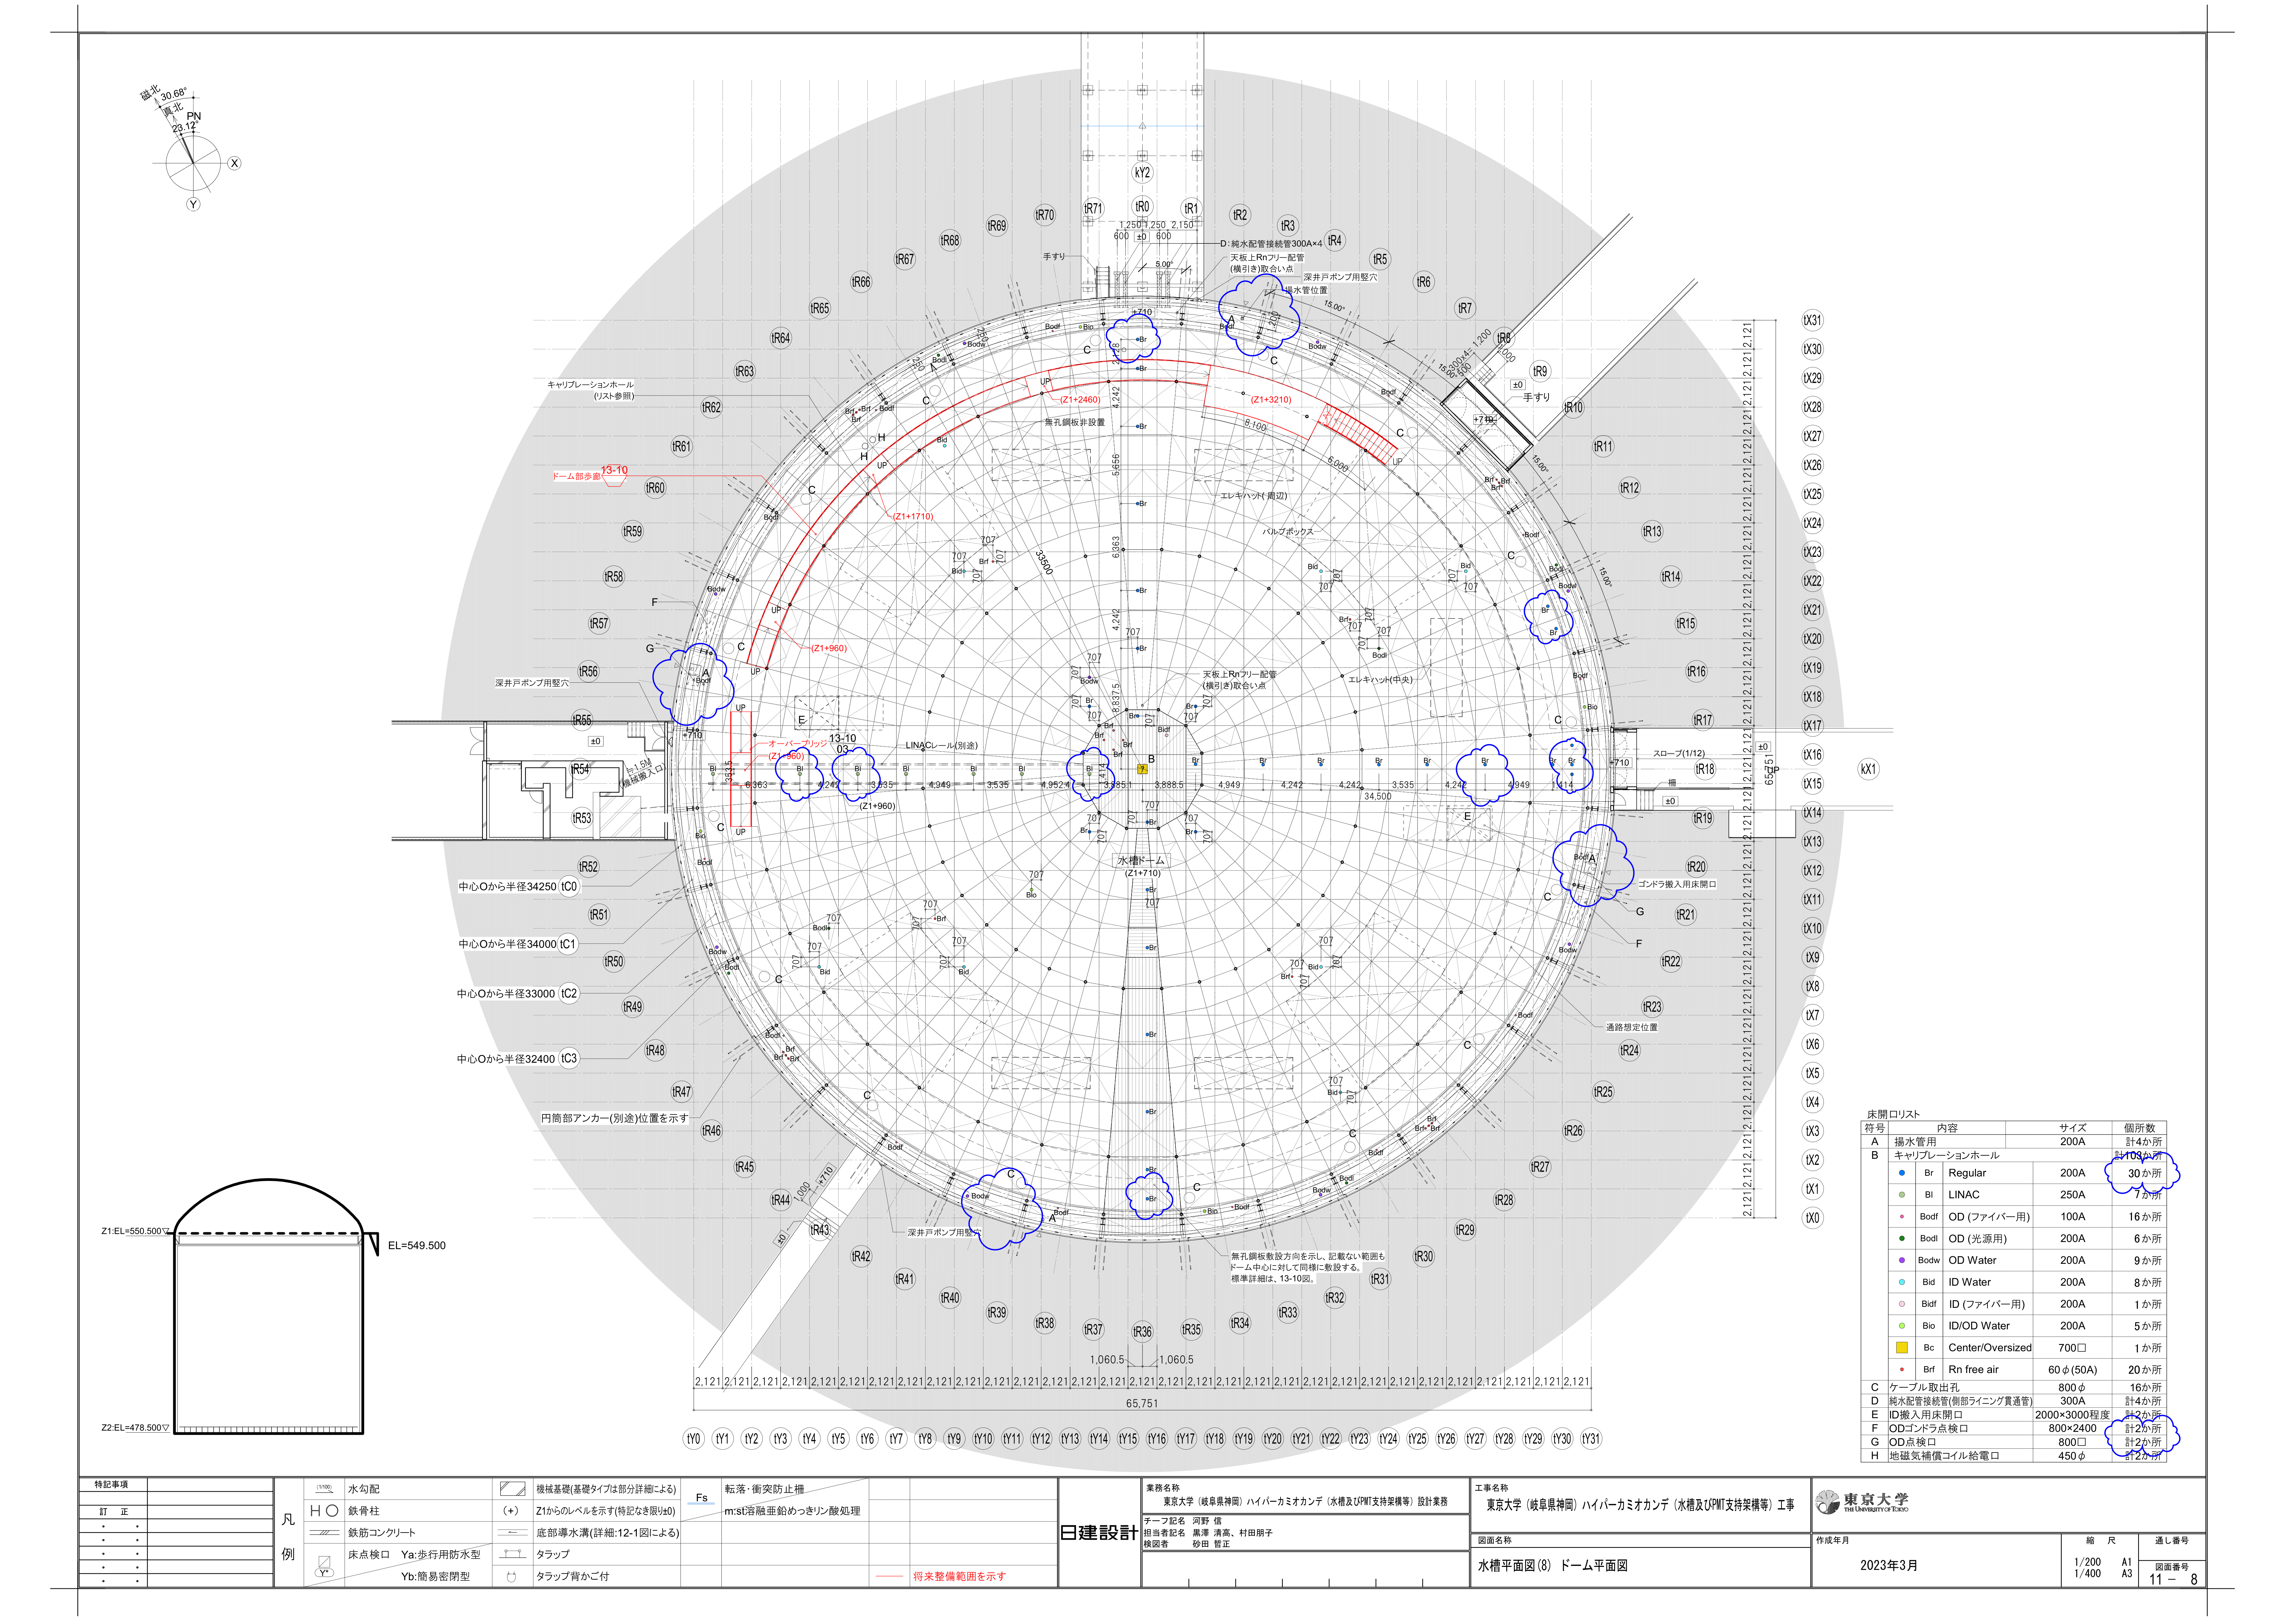
\includegraphics[angle=90,width=\textwidth]{portMap}
\caption{Top down view of the HK experimental area on top of the tank, showing locations of various calibration and fibre ports.}\label{fig:ports}
\end{figure}
\FloatBarrier
In order to limit the effect of potential damage to fibres, these will be split into in-tank and out-of-tank fibres. The fibres laid along the top deck will run from the calibration rack near the centre of the dome to patch panels next to the OD fibre ports. Being on the deck where there will be foot traffic for up to 20 years, the out-of-tank fibres are most likely to get damaged. Keeping them separate to the in-tank fibres makes replacing damaged fibres much easier, as it would be implausible to replace the in-tank fibres.

The initial preference for the fibre layout was to keep all fibre lengths the same. While this would involve many injectors being attached to fibres that were unnecessarily long, it would mean that the attenuation, dispersion and timing delays of pulses sent to all injectors would be constant. However, during the process of obtaining quotes, it was discovered that manufacturing a large number of fibres over 100~m would be problematic for the FP400URT, as draw lengths above 100~m are rare. This is problematic as lengths of $\sim$120~m are required to reach from the OD fibre ports to the centre of the bottom end-cap. To work around this, in-tank fibres will be split into two parts, one extending to the bottom of the barrel, and another extending across the bottom end-cap. Connectors will be installed on the bottom corners of the tank to facilitate this.

With multiple in-tank fibres needing to be connected together to reach the injectors on the bottom end-cap, it no longer makes sense to make all injector path lengths the same. Therefore, the required lengths need to be calculated for each section, based on deployment method and path taken. 

\subsection{Injector Cell Locations}\label{sec:lengths:sub:inj}
\subsubsection{Barrel Injectors}\label{sec:lengths:sub:inj:sub:barrel}

As shown in \cref{fig:IDmap}, the ideal ID injector layout features seven injector layers in the ID, equally separated. In reality, injector locations will be constrained by the available cells not already occupied by the PMTs, cable drums or various kinds of electronics vessels within the PMT support structure. 
\begin{figure}[h]
\centering
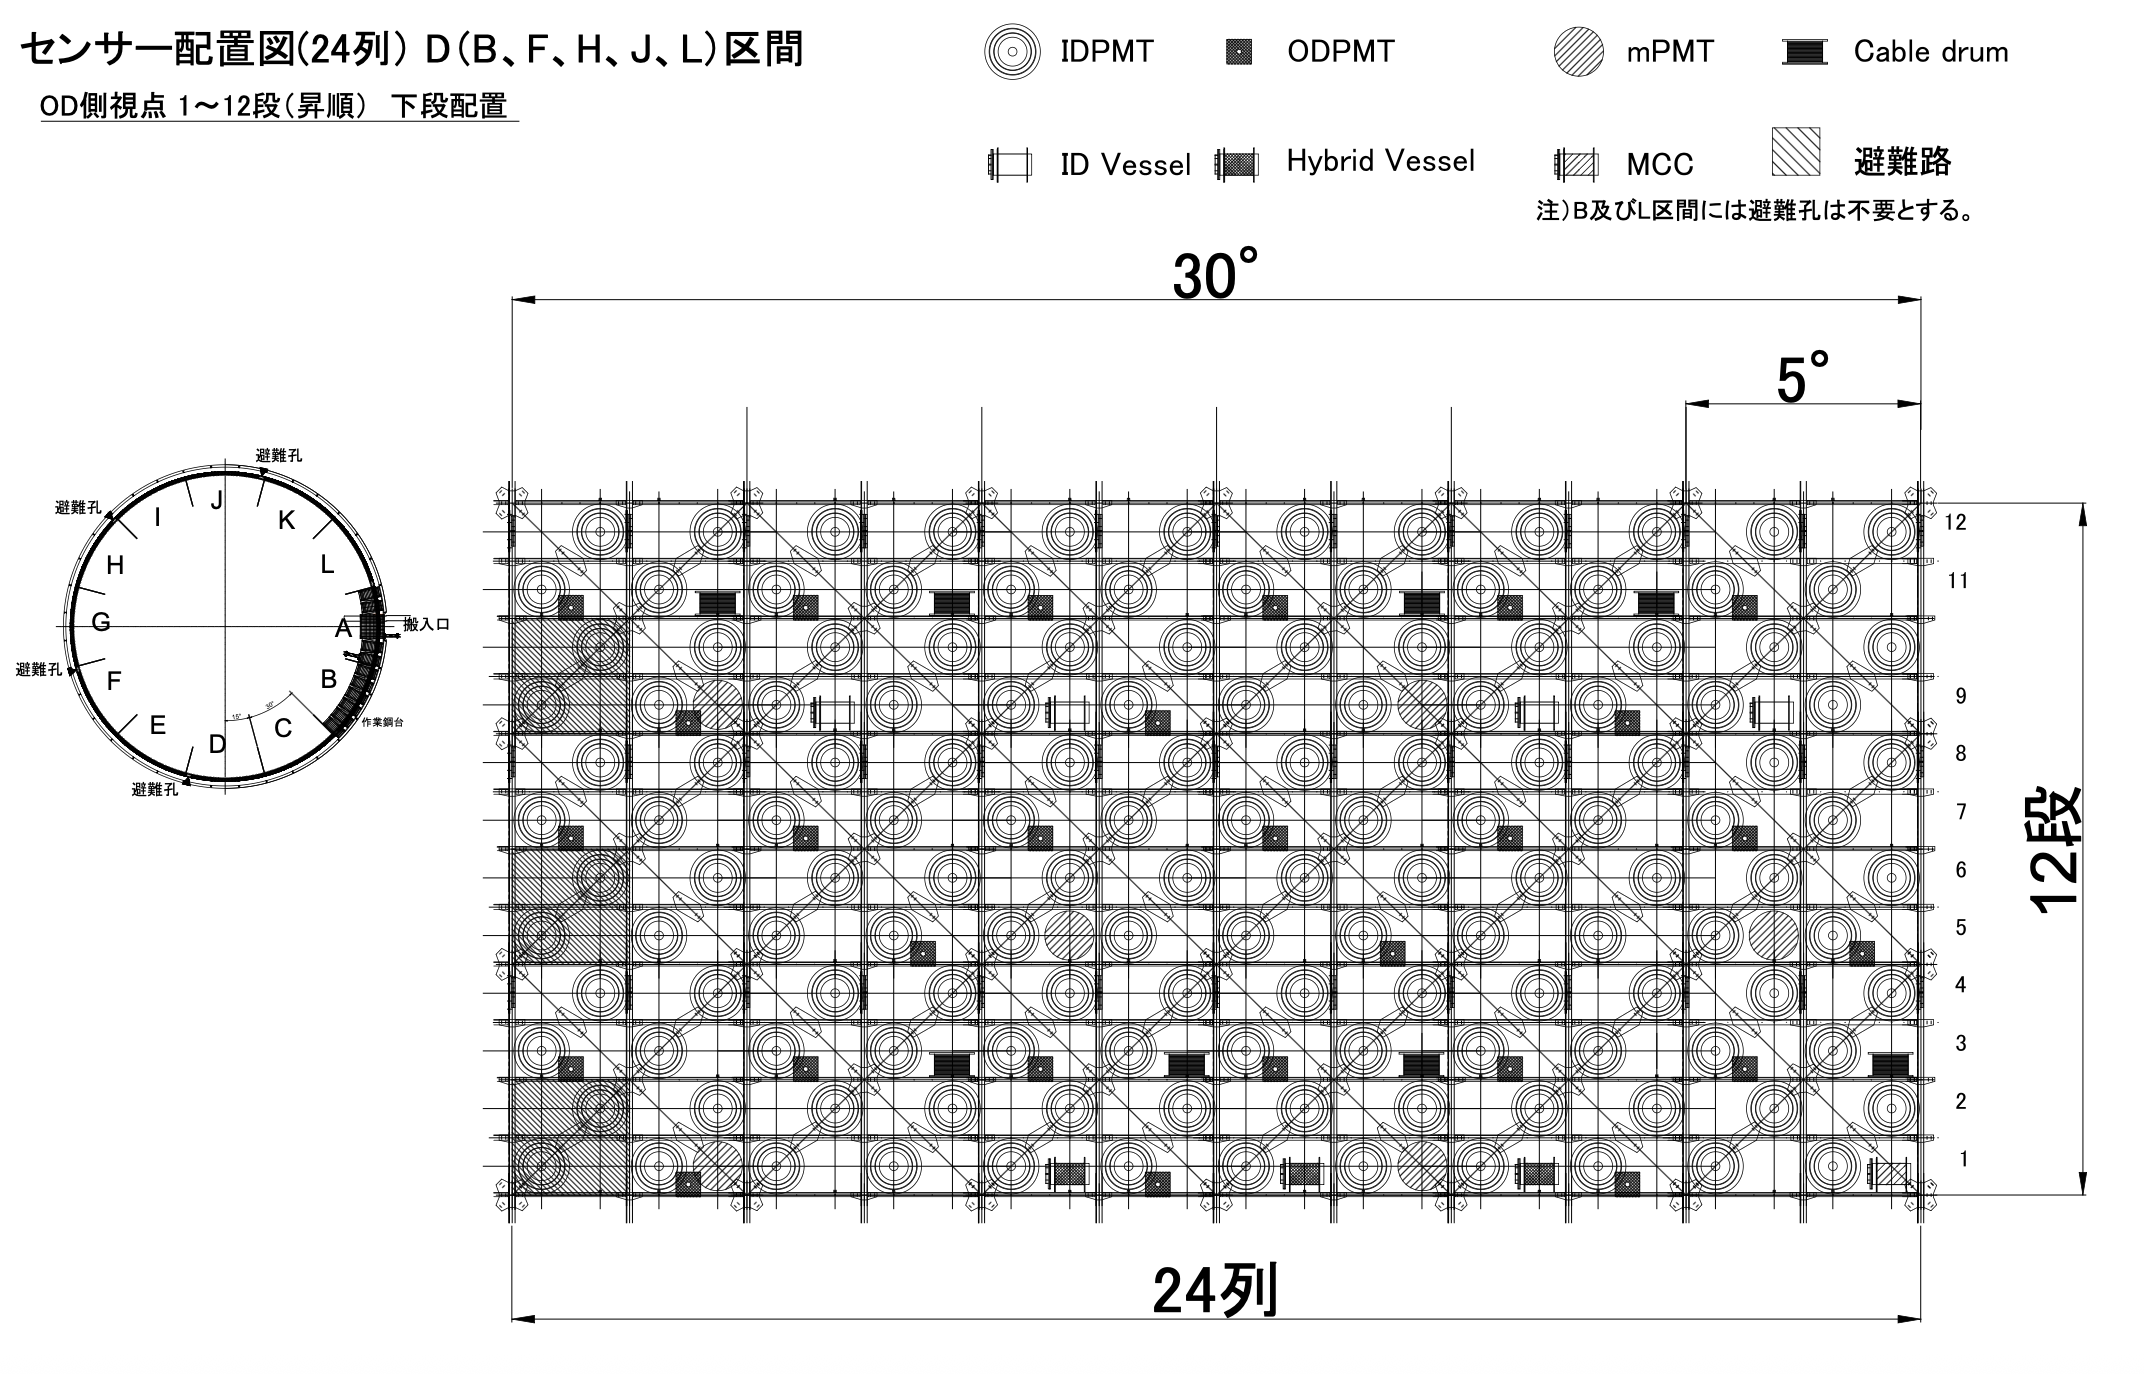
\includegraphics[width=0.9\textwidth]{barrelStructureDiagram.png}
\caption{Diagram showing cells 1-12 of a 30\degree\ section of the barrel PMT support structure, with fixed locations of components marked, as seen from the OD side of the structure.}\label{fig:barrelDiagram}
\end{figure}
\cref{fig:barrelDiagram} shows an example of this, for the bottom 12 cells of a 30\degree\ section of the barrel PMT support structure. There will be a total of 92 cells in the vertical direction. During construction, the barrel PMT support frame will be constructed in layers of four cells at a time. Once the full layer is complete and the respective components installed, the layer will be raised, and the next four cells constructed underneath. During construction of each four-cell layer, scaffolding will be required to work on the top two cells. To avoid this, installing injectors in the bottom two cells of each four-cell layer is planned. As the bottom cell of each layer is often dominated by electronics vessels, the second cell is preferable for injector locations. Dividing the total height into eight parts and taking the closest second layer yields the vertical cells given in \cref{tab:injvertical}. This results in a set of seven vertical cells symmetrical around cell 46, the top of which is at the centre of the tank. \cref{tab:injvertical} also lists the $z$ position of the bottom of the cell, using cell heights of 707~mm and again treating the top of cell 46 as $z=0$~mm. To get the injector $z$ coordinates an offset is added to each, accounting for the 125~mm width of the horizontal bars, and then assuming an extra 50~mm to account for diffuser mounting and radius.

\begin{table}[h!]
\centering
\begin{tabular}{cccc} \toprule
ID vertical label	&	Vertical cell	&	Cell $z$ position (mm)	&	Injector $z$ position (mm)	\\ \midrule
1					&		82			&		24745		&	24857.5	\\
2					&		70			&		16261		&	16373.5	\\
3					&		58			&		7777		&	7889.5	\\
4					&		46			&		-707		&	-594.5	\\
5					&		34			&		-9191		&	-9078.5	\\
6					&		22			&		-17675		&	-17562.5	\\
7					&		10			&		-26159		&	-26056.5	\\ \bottomrule
\end{tabular}
\caption{Vertical cell locations for both ID and OD barrel injectors. Cell $z$ position is defined as the bottom of the cell, and injector position assumes the injector being installed at the bottom of the cell, accounting for the width of horizontal bars and radius of injectors.}\label{tab:injvertical}
\end{table}

To define the horizontal location of cells, the radial labelling of the vertical support struts shown in \cref{fig:ports} is used, starting from tR0 and running to tR71 in the clockwise direction. Between each of these supports is a 5\degree\ angle, containing four cells. As no standard cell labelling currently exists in the horizontal, we label each cell 1 through 4, again in the clockwise direction, resulting in a horizontal cell label of the form tR$X.Y$, where $X\in\{0..71\}$ and $Y\in\{1..4\}$. As \cref{fig:barrelDiagram} is viewed from the OD side, vertical support labels and cell numbers increase from right to left.{\bf These cell addresses will be updated once a common system is decided within the integration group.}

As one column of ID injectors will coincide with the position of the Korean LI system, the horizontal positions are dictated by this. The Korean LI system will be installed between the two regular calibration ports (labelled `Br' in \cref{fig:barrelDiagram}) either side of tR14. Based on the previous requirements for cell choice, tR13.4 is the optimal choice for injector placement in this region, for the Korean LI and the ID LI optics. Placing LI ID injectors at every 90\degree\ this sets the remaining horizontal cell locations as tR31.4, tR49.4 and tR67.4.

The OD diffuser ideal positions are shown in \cref{fig:ODdiffmap}, where again there are seven vertical positions within the barrel. To simplify installation, the vertical positions for the ID and OD diffusers in the barrel will be aligned. As each layer of OD barrel diffusers is offset from the previous by 15\degree , this results in OD diffusers in the same cells as ID injectors for only layers 1, 3, 5 and 7. Starting from the overlap cells, and placing 12 diffusers in each layer (one every 30\degree), results in the OD diffuser barrel cell locations listed in \cref{tab:ODdiffBarrel}.
\begin{table}[h!]
\centering
\begin{tabular}{c|cc} \toprule
Vertical label 			& 1, 3, 5, 7 & 2, 4, 6 \\ \midrule
\multirow{12}{*}{Horizontal cell}	&	tR1.4	&	tR4.4 	\\
						&	tR7.4	&	tR10.4	\\
						&	tR13.4	&	tR16.4	\\
						&	tR19.4	&	tR22.4	\\
						&	tR25.4	&	tR28.4	\\
						&	tR31.4	&	tR34.4	\\
						&	tR37.4	&	tR40.4	\\
						&	tR43.4	&	tR46.4	\\
						&	tR49.4	&	tR52.4	\\
						&	tR55.4	&	tR58.4	\\
						&	tR61.4	&	tR64.4	\\
						&	tR67.4	&	tR70.4	\\ \bottomrule
\end{tabular}
\caption{Cell locations for OD barrel diffusers.}\label{tab:ODdiffBarrel}
\end{table}

While the exact positions of the 12 OD collimators are yet to be set, the rough locations for mounting have been decided. Three will be installed on the edge of the top end-cap, while the other nine will be installed on the edge of the bottom end-cap.

\subsubsection{End-cap Injectors}

For the ID injectors, the top-end cap will have a single location. The diffuser and collimator will be installed through the ID fibre port, labelled `Bidf' in \cref{fig:ports}. Only one position here is needed, as the injectors can easily be removed in the case of any faults. For the bottom end-cap this is of course not possible, and so four sets of injectors will be installed around the centre for degeneracy. A diagram of an end-cap is shown in \cref{fig:endcapmap}. The locations of PMTs and electronics vessels shown will be the same for both top and bottom. Only the ports (shown in yellow) are unique to the top end-cap.

\begin{figure}[h]
\centering
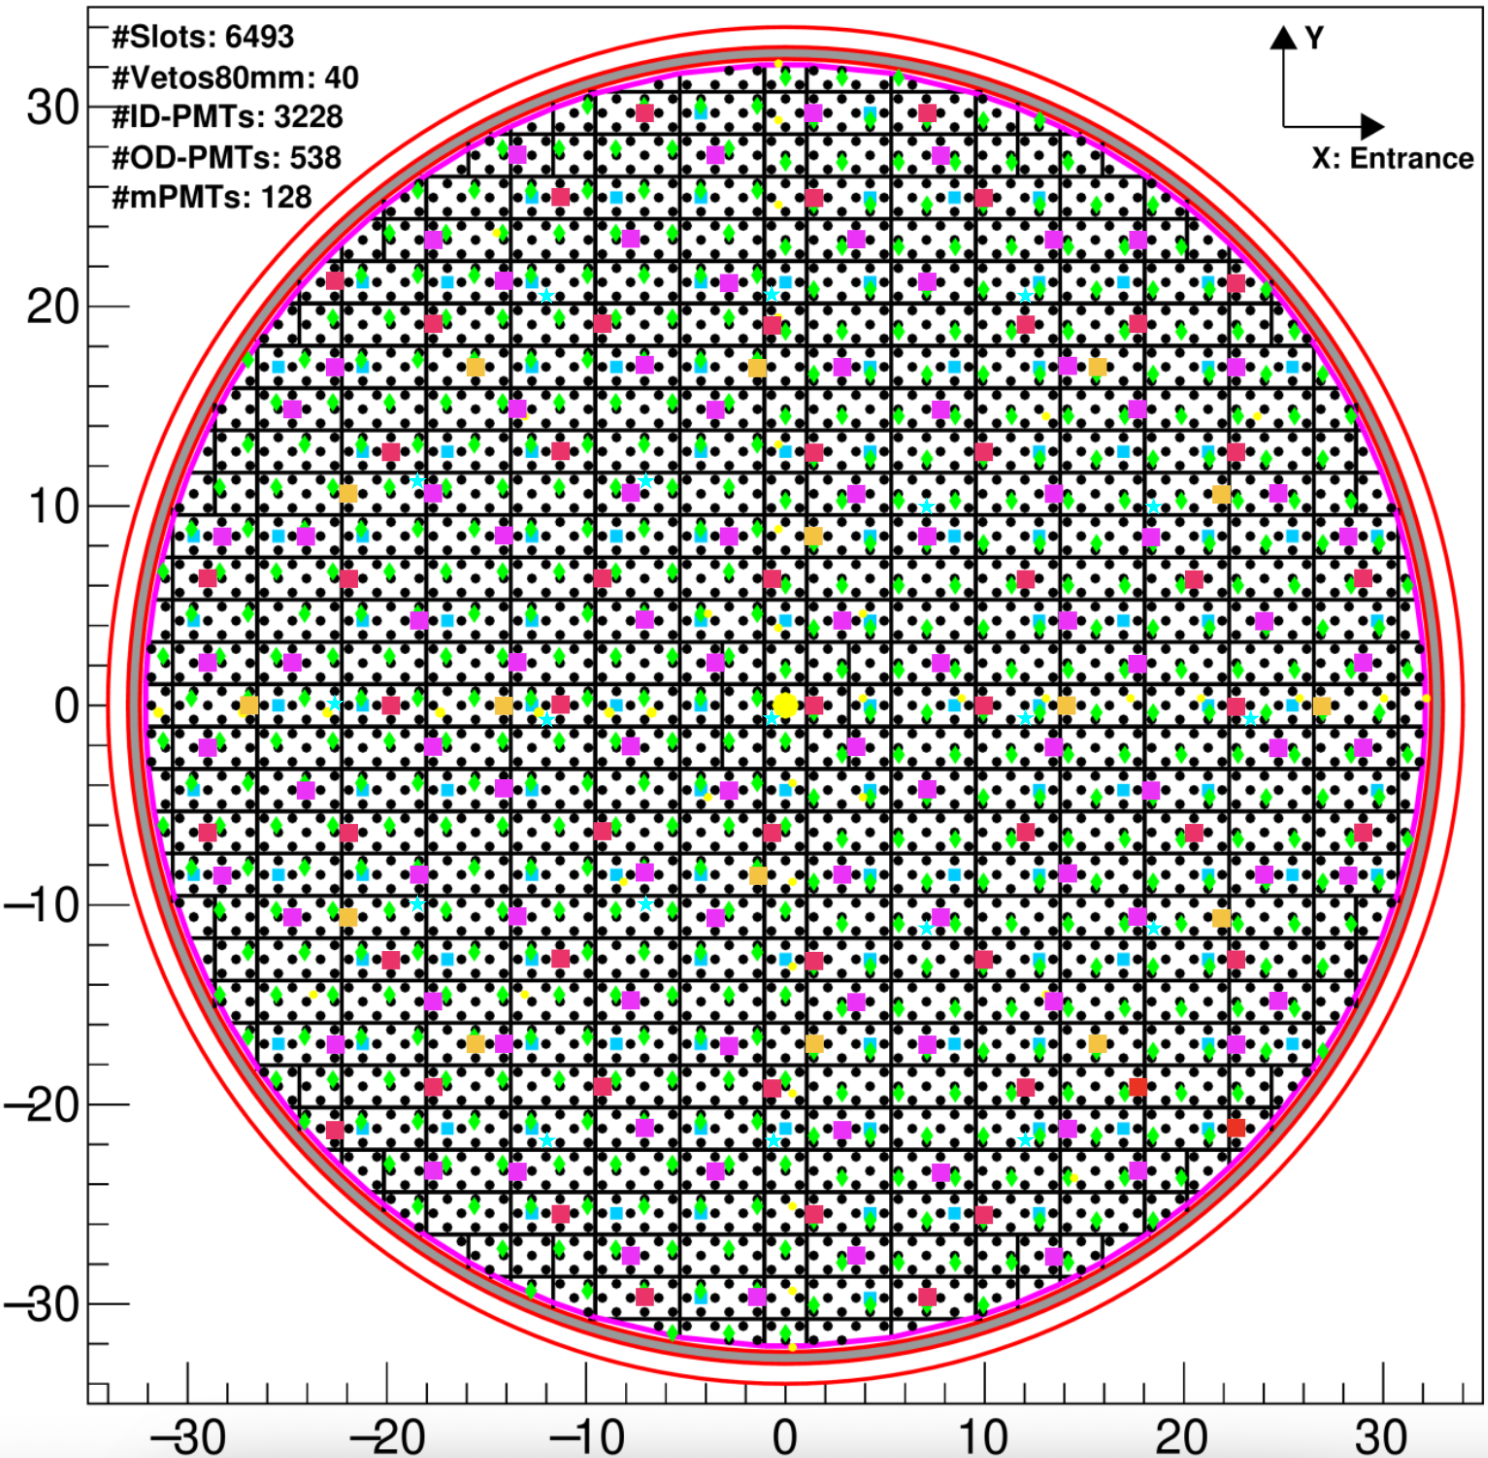
\includegraphics[width=0.9\textwidth]{endcapODdiff.png}
\caption{Diagram of PMT support structure end-cap, with a variety of components' locations shown. Other than calibration ports (yellow circles), mapping is the same for both top and bottom end-caps. The location of OD diffusers is shown with cyan stars.}\label{fig:endcapmap}
\end{figure}

For the OD, 19 diffusers will be installed on each end-cap. The locations of these, which are again same for top and bottom, are shown in \cref{fig:endcapmap}, denoted by cyan stars. These positions are chosen to match as closely as possible to the `ideal' layout shown in \cref{fig:ODdiffmap}. {\bf Exact cell locations will be provided once a cell address scheme is decided upon by integration group}.


\subsection{Fibre Paths}

With the locations of the injectors decided, the routes of fibre optic cables to said injectors can be planned, and the required lengths of each set of fibres obtained. Installation of the majority of fibres will take place after construction of the PMT support structure is completed. A small team of experts will enter the tank in the OD gondola, using this to route fibres around the tank. Given the size of the Hyper-K tank, and the low speed of a gondola (initial designs estimate this at 0.2~ms$^{-1}$), many decisions made here are in an effort to make installation as efficient as possible.

\subsubsection{Top Deck}\label{sec:lengths:sub:len:sub:deck}

This set of fibres is used to run from the calibration racks near the centre of the top deck, to respective OD calibration ports around the edge, where they will attach to patch panels. This will be done for all injectors except for the top ID injectors, and top OD diffusers. The preferred method for installation is for the fibres to be laid into cable trays underneath the deck, to limit the chance of breakage from exposure to foot traffic. In mapping these routes out it is assumed that the fibre can travel in a straight line from rack to port, with the exception of having to avoid any structures that penetrate the deck to the tank, such as ports and gondola hatches. The proposed routing is shown in \cref{fig:deckFibreMap}, though the exact location within the calibration area marked in blue that the fibres would meet is as yet unknown. The only fibres which cannot travel in a straight line are those to ODF5 and ODF13, as they have to bend around the marked ID gondola hatches. Using this as a guide, the required fibre lengths can be calculated. As the point that the fibres will exit at the calibration rack is unknown, the unit 2121$\times$2121~mm square is highlighted, and the distance to the closest edge of this measured. To account for the unknown distance within the square, and any vertical travel required up the calibration rack, an addition of 5~m will then be applied to every required length. 
\begin{figure}[ht!]
\centering
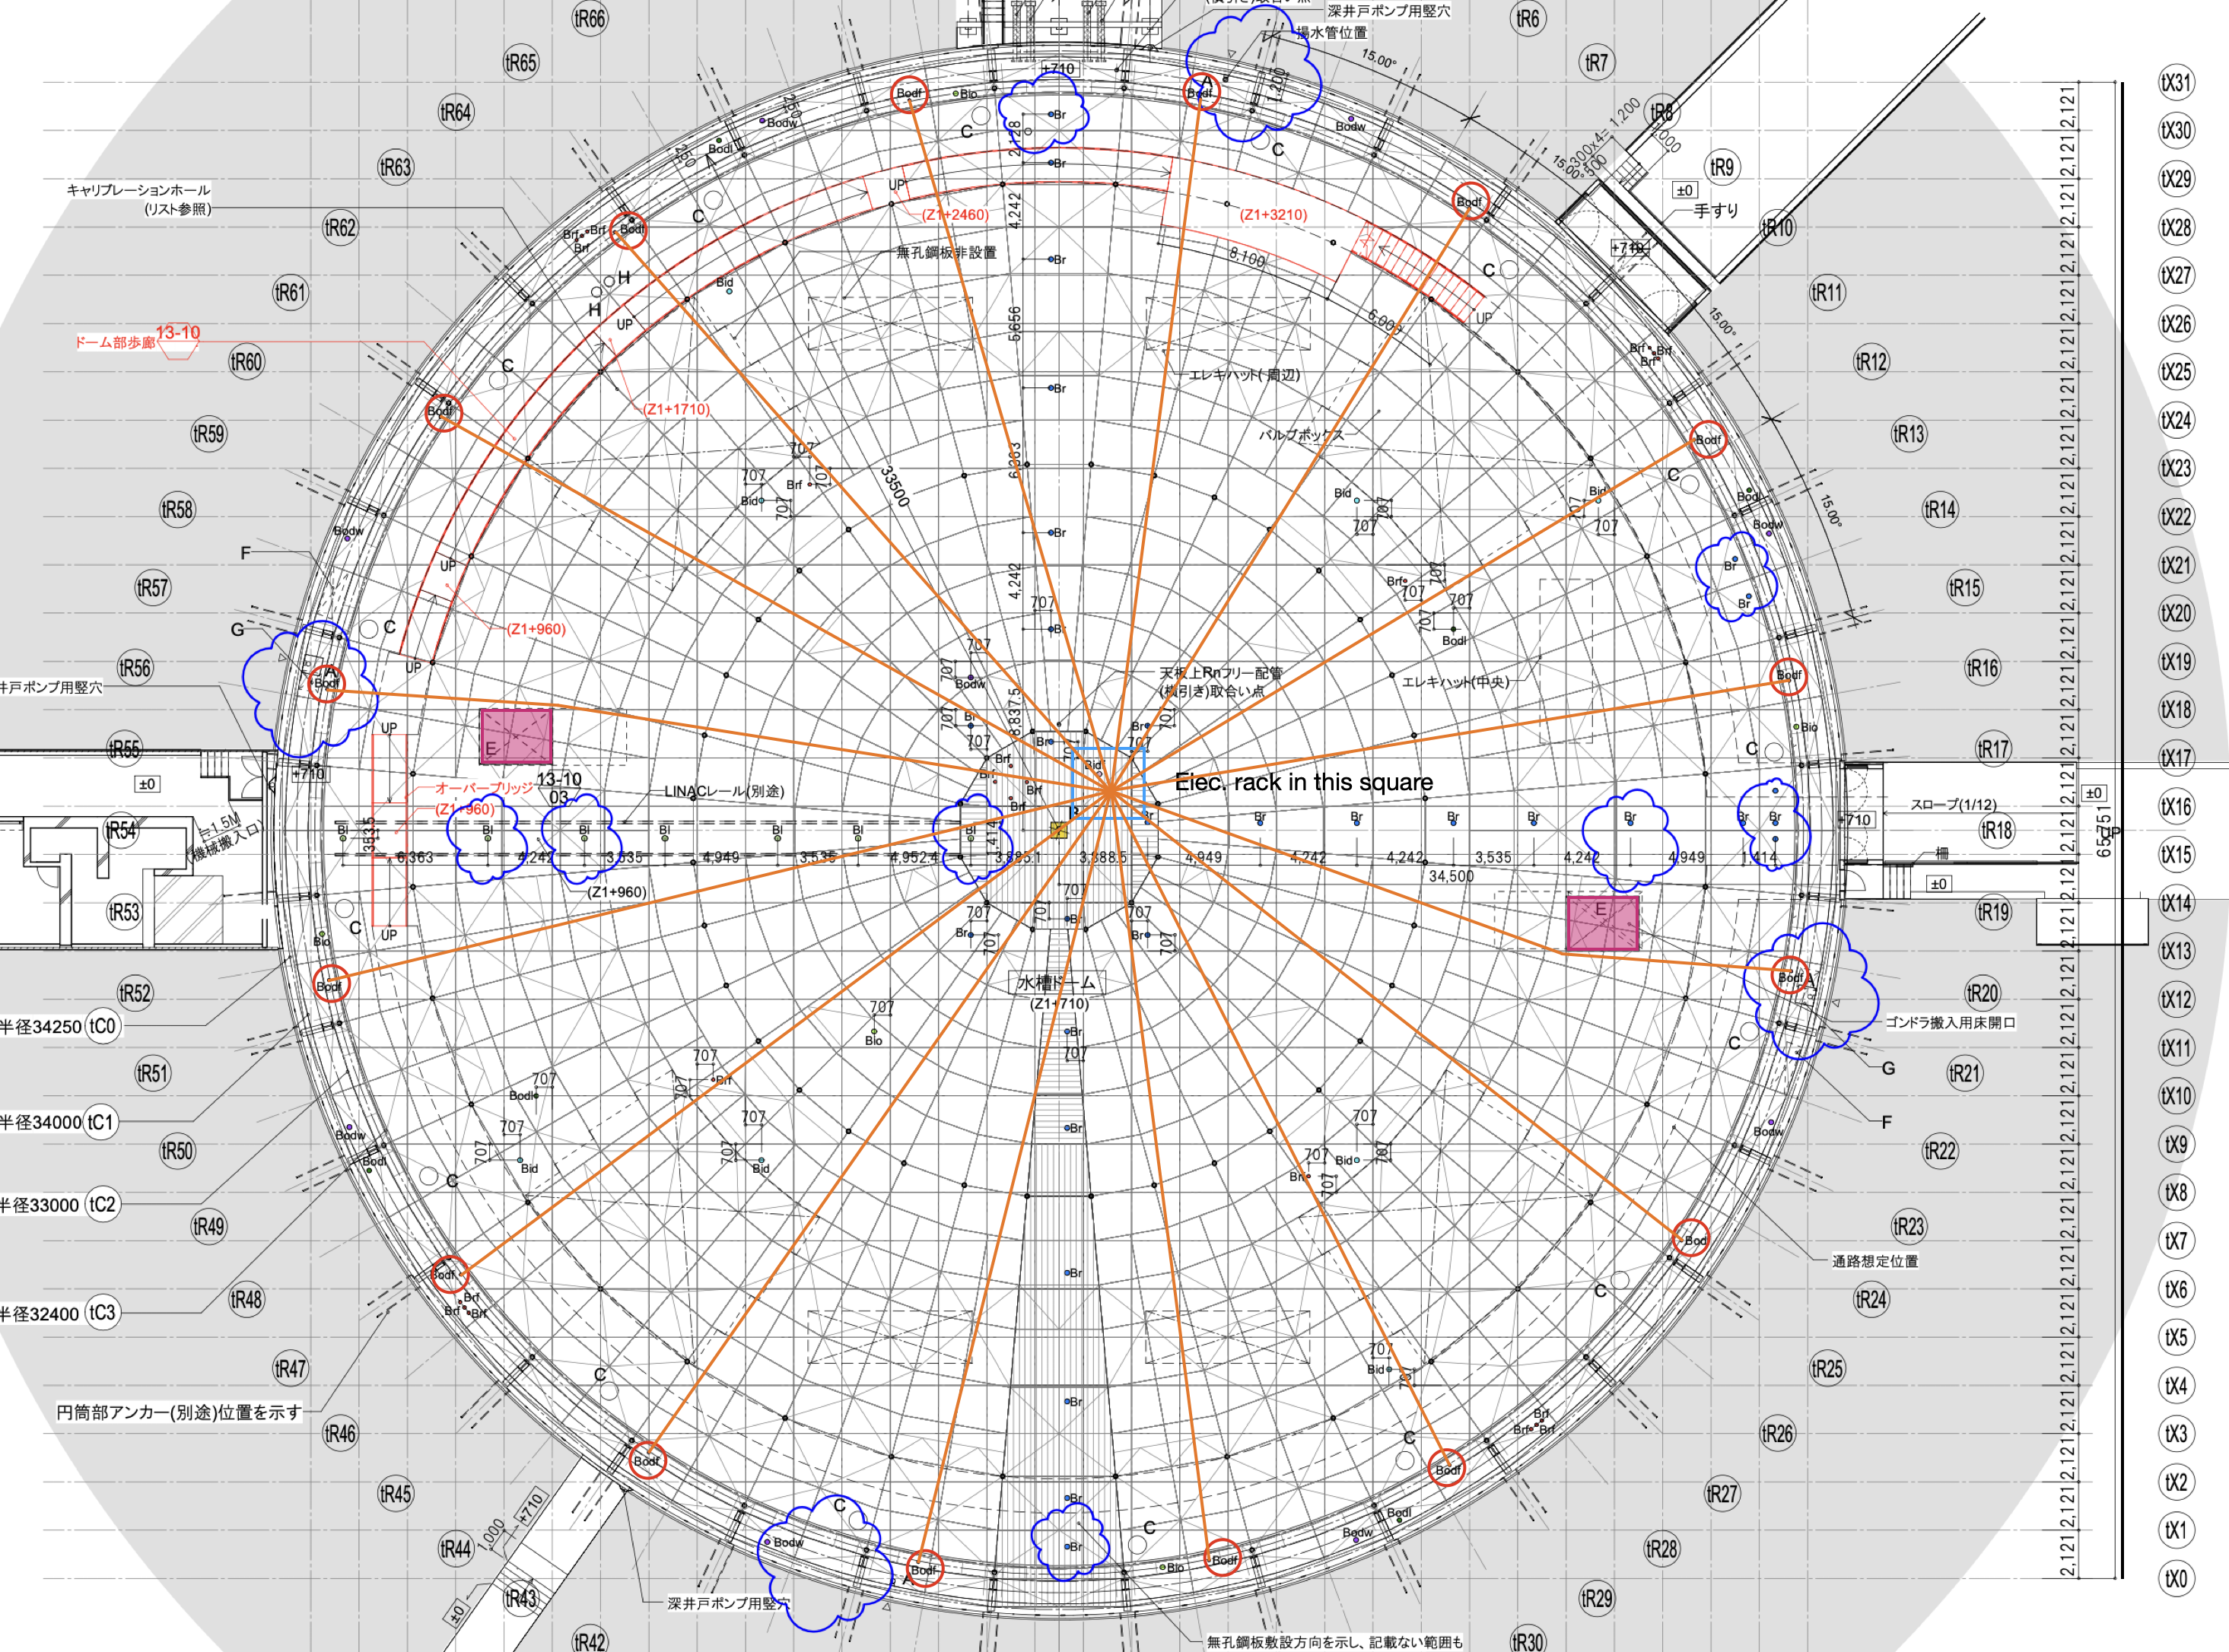
\includegraphics[width=0.8\textwidth]{deckFibreMap}
\caption{Diagram of fibre routing below deck from calibration rack to OD fibre ports. OD ports are circled in red, ID gondola hatches outlined in purple, and the blue square shows a $\sim 3\times 3$~m square where the calibration racks will be. Orange lines show the proposed fibre routes.}\label{fig:deckFibreMap}
\end{figure}
\begin{figure}[h!]
\centering
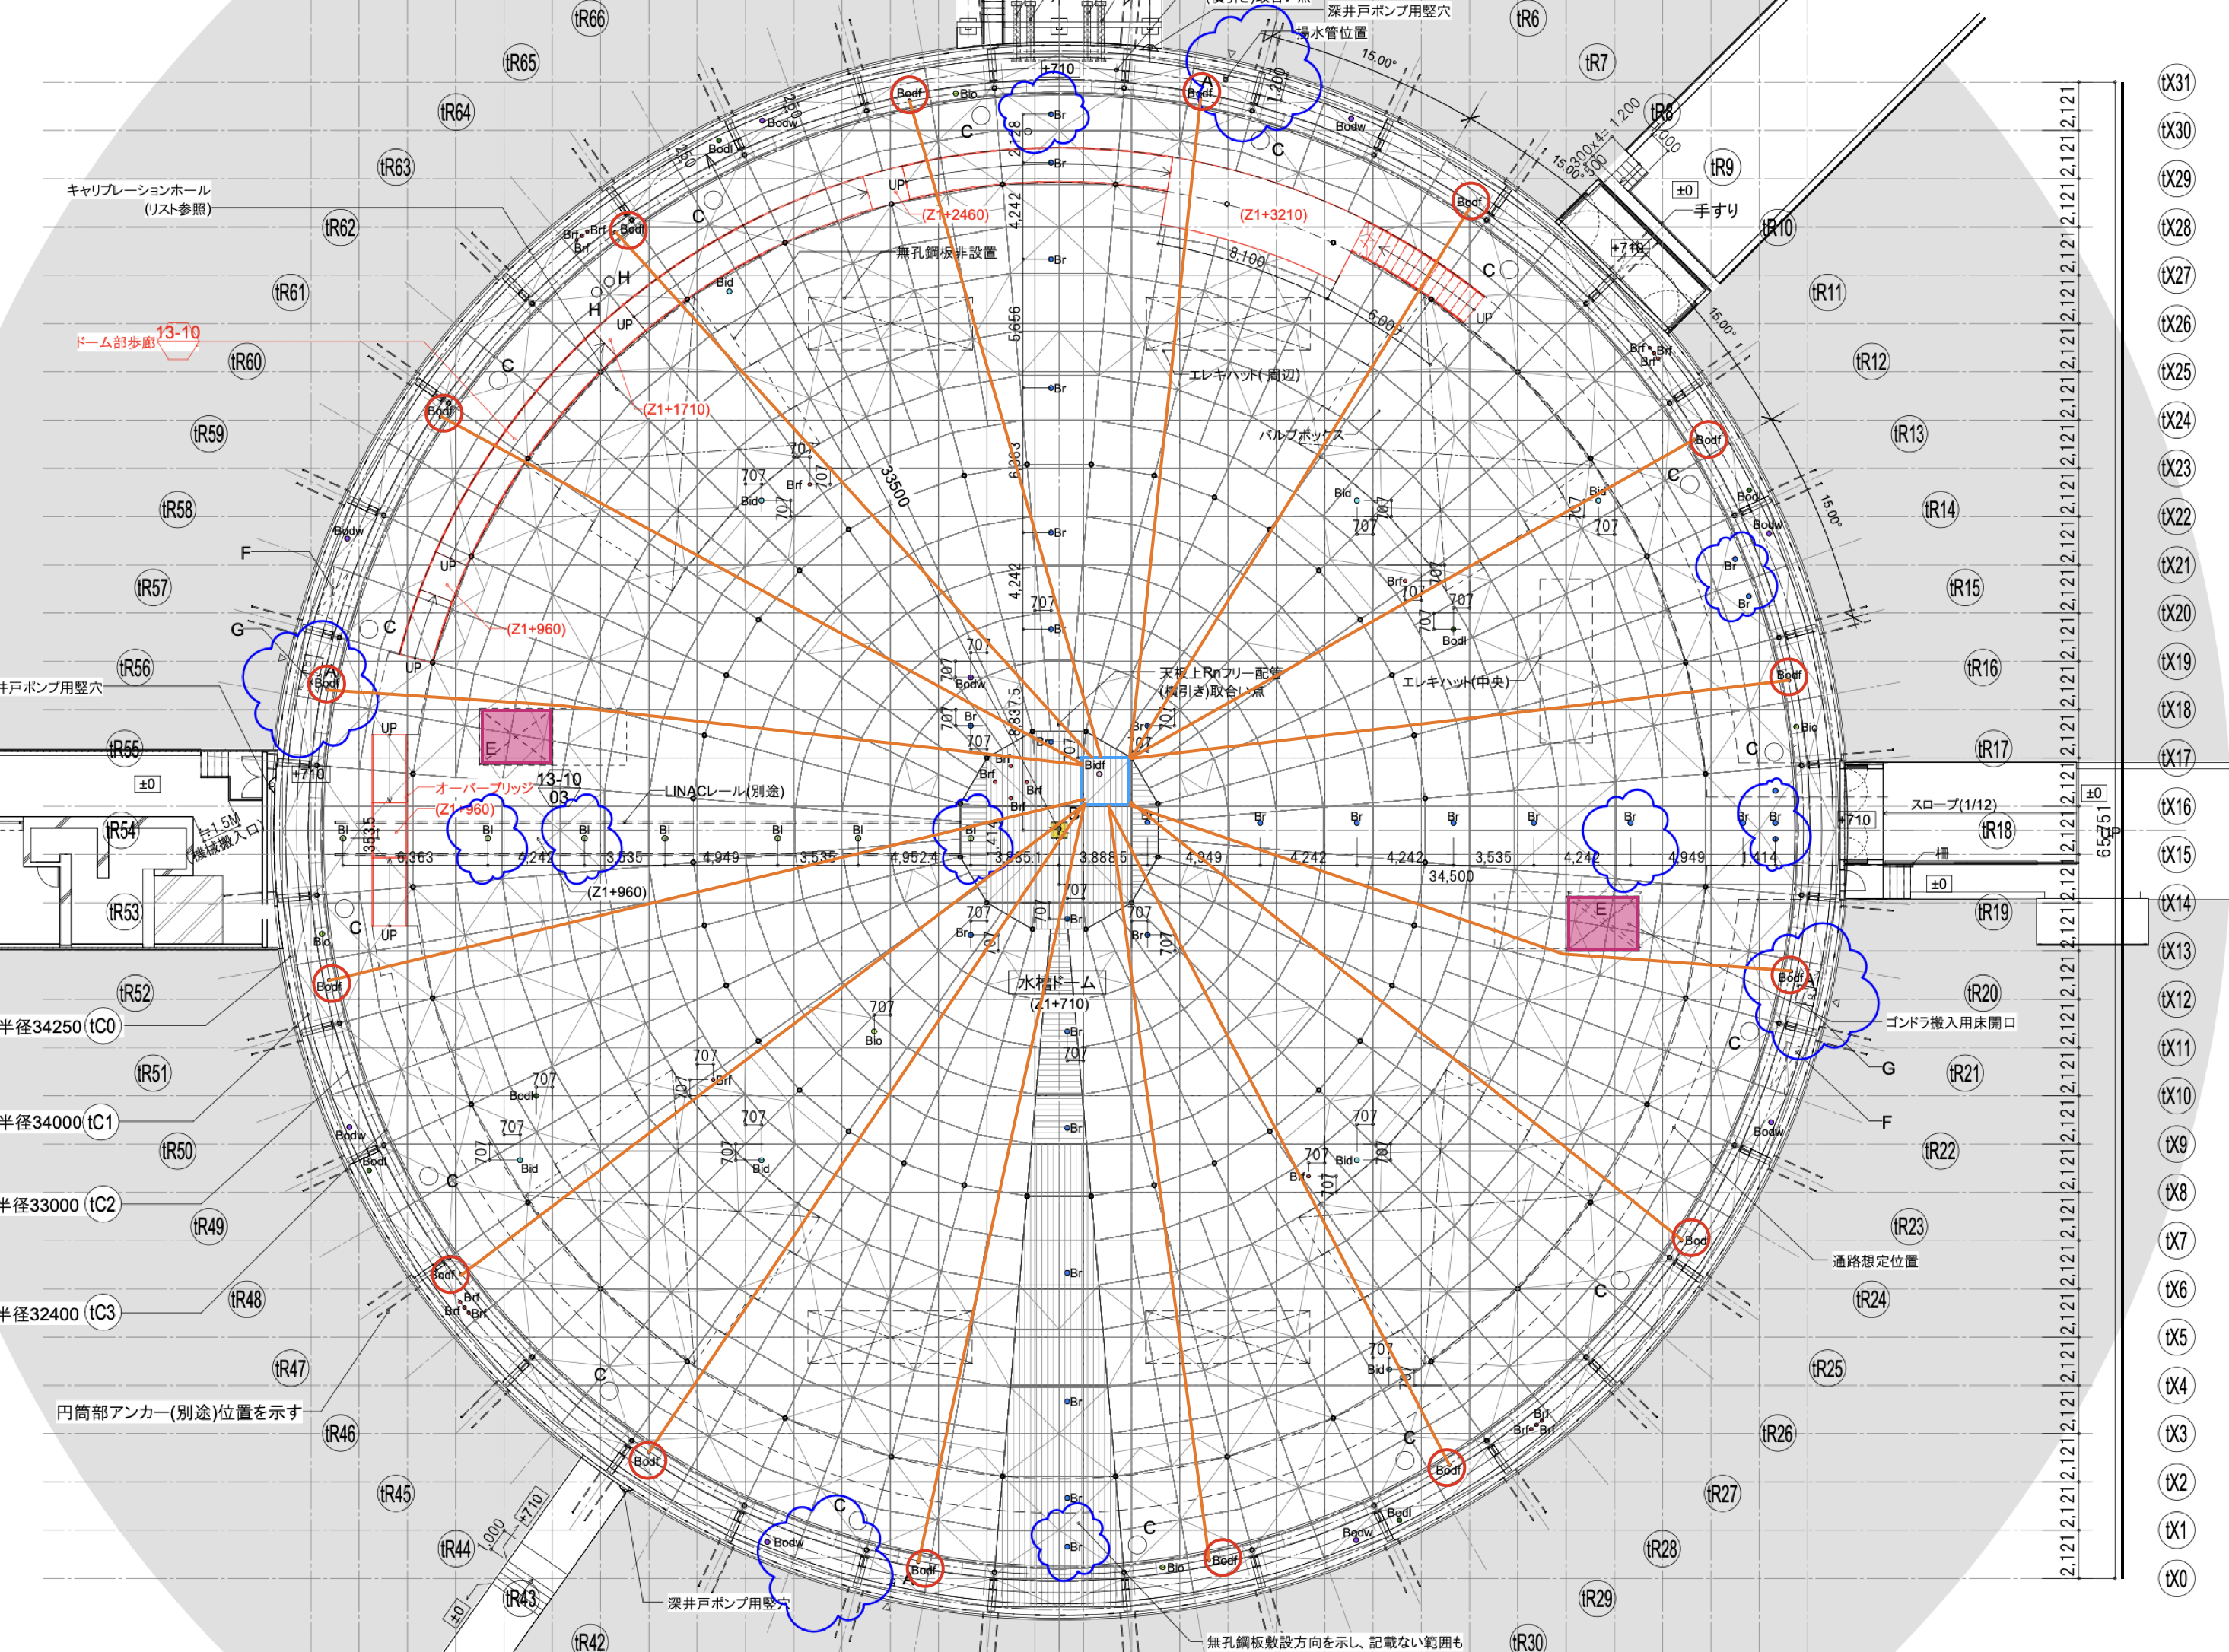
\includegraphics[width=0.8\textwidth]{deckFibreMeasure}
\caption{Same as \cref{fig:deckFibreMap}, except the blue square outlines the $\sim 2\times 2$~m square within which the fibres could potentially exit the deck, as the exact location of the calibration rack is not known. In this case the orange lines are used to measure distance from respective calibration port to the edge blue square. This is not the map used for fibre routing itself.}\label{fig:deckFibreMeasure}
\end{figure}
The actual measurement of each fibre is done by the pixel length of each line from rack to port. The total diameter of the tank is measured to be 984~pt. As this is shown in \cref{fig:deckFibreMeasure} to be 65751~mm, this equates to $1~\text{pt} = 66.82~\text{mm} \simeq 67~\text{mm}$. Using this, the required length of each fibre can be calculated. These values are summarised in \cref{tab:deckFibreLen}.
\begin{center}
\begin{table}[h]
\begin{tabular}{ccc} \toprule
Port ODF no. &	Length [pt]	&	Length [mm] \\ \midrule
	1			&	437			&	29279		\\
	2			&	426			&	28542		\\
	3			&	427			&	28609		\\
	4			&	437			&	29279		\\
	5			&$152+301=453$	&	30351		\\
	6			&	465			&	31155		\\
	7			&	489			&	32763		\\
	8			&	503			&	33701		\\
	\bottomrule
\end{tabular}
\begin{tabular}{ccc} \toprule
Port ODF no. &	Length [pt]	&	Length [mm] \\ \midrule
	9			&	512			&	34304		\\
	10			&	515			&	34505		\\
	11			&	516			&	34572		\\
	12			&	513			&	34371		\\
	13			&$153+349=502$	&	33634		\\
	14			&	481			&	32227		\\
	15			&	468			&	31356		\\
	16			&	451			&	30217		\\
	\bottomrule
\end{tabular}
\caption{Required length of fibre to reach from each OD fibre port to the 2121$\times$2121~mm square the calibration rack is assumed to be in.}\label{tab:deckFibreLen}
\end{table}
\end{center}
The maximum length requirement found here is 34572~mm, to get to ODF 11. Adding the 5~m to account for reaching the calibration rack and travelling vertically to the specific crate gives a total distance of 39572~mm. This can then be rounded to 42~m for safety, and to ensure the fibres have some slack in them. As both ends of the fibres will connect to patch panels, each end of the fibre should have an FC/PC connector, for both fibre types.

\subsubsection{Barrel Fibres}\label{sec:lengths:sub:len:sub:barrel}

There are two sets of fibres which need to run down the side of the barrel: those that connect to barrel injectors, and those that must run to the bottom of the tank to reach bottom end-cap injectors. As these will both take the same paths down the vertical supports, they are included together here. 

To route these fibres to either a barrel injector or bottom end-cap, the fibres will run through one of the 16 OD calibration ports. These ports extend 1200~mm below the top of the tank, into the dead region of the PMT support structure. At the point where the fibres exit the port, they will be routed to one of the two neighbouring vertical supports. The support chosen will not necessarily be the closest one, as choices should be optimised for efficient installation. The mapping between horizontal cell location, fibre port, and vertical support to route down is shown in the first three columns of \cref{tab:barrelInjPorts}.
\begin{table}
\centering
\begin{tabular}{cccc}\toprule
Inj. cell	&	ODF	&	Vertical to route down	&	Port to inj. angle	[\degree ]	\\ \midrule
tR1.4		&	1	&		2					&		\phantom{0}0.625		\\
tR4.4		&	2	&		6					&		\phantom{0}5.625		\\
tR7.4		&	2	&		6					&		\phantom{0}9.375		\\
tR10.4		&	3	&		12					&		\phantom{0}5.625		\\
tR13.4		&	4	&		15					&		\phantom{0}5.625		\\
tR16.4		&	4	&		15					&		\phantom{0}9.375		\\
tR19.4		&	5	&		20					&		\phantom{0}0.625		\\
tR22.4		&	6	&		25					&		10.625		\\
tR25.4		&	6	&		25					&		\phantom{0}4.375		\\
tR28.4		&	7	&		29					&		\phantom{0}0.625		\\
tR31.4		&	8	&		33					&		\phantom{0}5.625		\\
tR34.4		&	8	&		33					&		\phantom{0}9.375		\\
tR37.4		&	9	&		38					&		\phantom{0}0.625		\\
tR40.4		&	10	&		43					&		10.625		\\
tR43.4		&	10	&		43					&		\phantom{0}4.375		\\
tR46.4		&	11	&		47					&		\phantom{0}0.625		\\
tR49.4		&	12	&		52					&		10.625		\\
tR52.4		&	12	&		52					&		\phantom{0}4.375		\\
tR55.4		&	13	&		57					&		\phantom{0}5.625		\\
tR58.4		&	13	&		57					&		\phantom{0}9.375		\\
tR61.4		&	14	&		61					&		\phantom{0}4.375		\\
tR64.4		&	15	&		65					&		\phantom{0}0.625		\\
tR67.4		&	16	&		70					&		10.625		\\
tR70.4		&	16	&		70					&		\phantom{0}4.375		\\ \bottomrule
\end{tabular}
\caption{List of all barrel injector horizontal cell locations, with corresponding OD fibre port to route through, vertical support to route down, and angle between the given vertical support and the injector cell. This assumes injector installation in centre of cell.}\label{tab:barrelInjPorts}
\end{table}
As should be clear from this, the majority of injectors will not have the fibre run directly down to them. Instead, each fibre will run down the respective vertical support until at the same horizontal level as the injector, before being running radially around the side of the detector to reach the injector cell. In both ID and OD cases this will be done on the outer edge of the support structure; for OD diffusers this is where they will be housed. For the ID injectors, a patch cable to span the dead region will have been installed at the same time as the injector housing itself, to avoid the person connecting the fibre having to reach out of the gondola into the dead region.

To calculate the maximum amount of additional fibre needed to account for this horizontal travel, the angular difference between each injector cell and the respective vertical support used to route down can be calculated. This is done assuming the injector is installed in the centre of a cell, with the values given in the final column of \cref{tab:barrelInjPorts}. Taking the maximum angular difference of 10.625\degree, an arc length of 6130~mm is found. The same has to be done for the distance between the OD fibre port and the vertical support. As the locations of the ports are not precisely documented, the maximum angular distance of 5\degree\ is taken, equating to 2885~mm. These additions will apply to all barrel injectors. For the fibres needed to reach the bottom, only the horizontal addition for port to vertical distance is required.

Vertical and total length requirements for the barrel fibres are easily found from the vertical cell locations given in \cref{tab:injvertical}, using a cell height of 707~mm, and a distance from the deck to top of cell 92 of 3935~mm. This again uses a bar width of 125~mm, and assumes a 50~mm offset to account for the height of the injector. The calculated values are shown \cref{tab:barrelLength}.
\begin{table}[h!]
\centering
\begin{tabular}{cccc}\toprule
Vertical label	&	Layer	&	Vertical dist. from deck [mm]	&	Total dist. from port [mm]	\\	\midrule
	1			&	82		&	11617.5							&	20632.5	\\
	2			&	70		&	20101.5							&	29116.5	\\	
	3			&	58		&	28585.5							&	37600.5	\\
	4			&	46		&	37069.5							&	46084.5	\\
	5			&	34		&	45553.5							&	54568.5	\\
	6			&	22		&	54037.5							&	63052.5	\\
	7			&	10		&	62521.5							&	71536.5	\\
	Bottom		&	0		&	70412.5							&	73297.5	\\ \bottomrule
\end{tabular}
\caption{Vertical and total travel distance to reach to a given layer of barrel injectors. Both distances are calculated from the deck, but the total distance takes into account maximum required travel from port to vertical and vertical to injector. Only the port to vertical distance is added for fibres extending to the bottom end-cap.}\label{tab:barrelLength}
\end{table}
These numbers show that the additional horizontal fibre required to reach from vertical supports to an injector cell is not a problem, as the maximum length case still comes from reaching to the bottom of the barrel. For contingency, and to allow fibres to not be kept taught, the maximum length requirement is rounded up to 76~m. For the ID system, all fibres will have FC/PC connectors on either end. This is the same for the OD system fibres which traverse the entire barrel depth to the bottom end-cap. For the fibres connecting to OD barrel diffusers however, these will be polished fibre on one end, as this is what has to be pushed into the back of the diffuser hemisphere.

The plans presented here are used to calculate the maximum required length. Rather than have all fibres that traverse the barrel the same length, an alternative option is to split into three sets of fibres so that the amount of excess fibre can be limited, particularly for the higher up injectors. In this case, there is one length for vertical labels 1 and 2, one for 3, 4 and 5, and one for 6, 7, and fibres to the bottom of the barrel. The lengths of these are calculated using the values from \cref{tab:barrelLength}, and are given in \cref{tab:barrelLengthSplit}. From both a cost and installation perspective, this case using three different lengths of fibre for the barrel injectors is the preferred method.
\begin{table}[h!]
\centering
\begin{tabular}{cc}\toprule
Region		&		Length [m]		\\ \midrule
1+2			&		32	\\
3+4+5		&		58	\\
6+7+bottom	&		76	\\ \bottomrule
\end{tabular}
\caption{Total length requirements for barrel fibres, in the case where lengths are split for different barrel regions to reduce excess fibre.}\label{tab:barrelLengthSplit}
\end{table}

As mentioned in \cref{sec:lengths:sub:inj:sub:barrel}, there will also be 12 OD collimators affixed to the barrel/end-cap edges; three on the top and nine on the bottom. The bottom collimators will require the aforementioned amount of fibre needed to reach the edge of the bottom end-cap. For the top ones, which will also be connected through the OD fibre ports, a length of 10~m will be enough to connect these.

\subsubsection{Bottom end-cap}\label{sec:lengths:sub:len:sub:bottom}

To reach the injectors on the bottom end-cap, a final set of fibres is required. These will run from the connectors installed on the bottom edge of the PMT support structure, to a given injector position. In order to simplify installation, the bottom end-cap cable mapping is optimised to only run from four vertical supports, minimising the number of times the gondola will need to traverse the full height of the tank. In doing this ODF4 is also avoided, as this is the port that the Korean injector fibres will also run through, and it is preferable to not overload a single port or vertical support with fibres.
\begin{figure}[h]
\centering
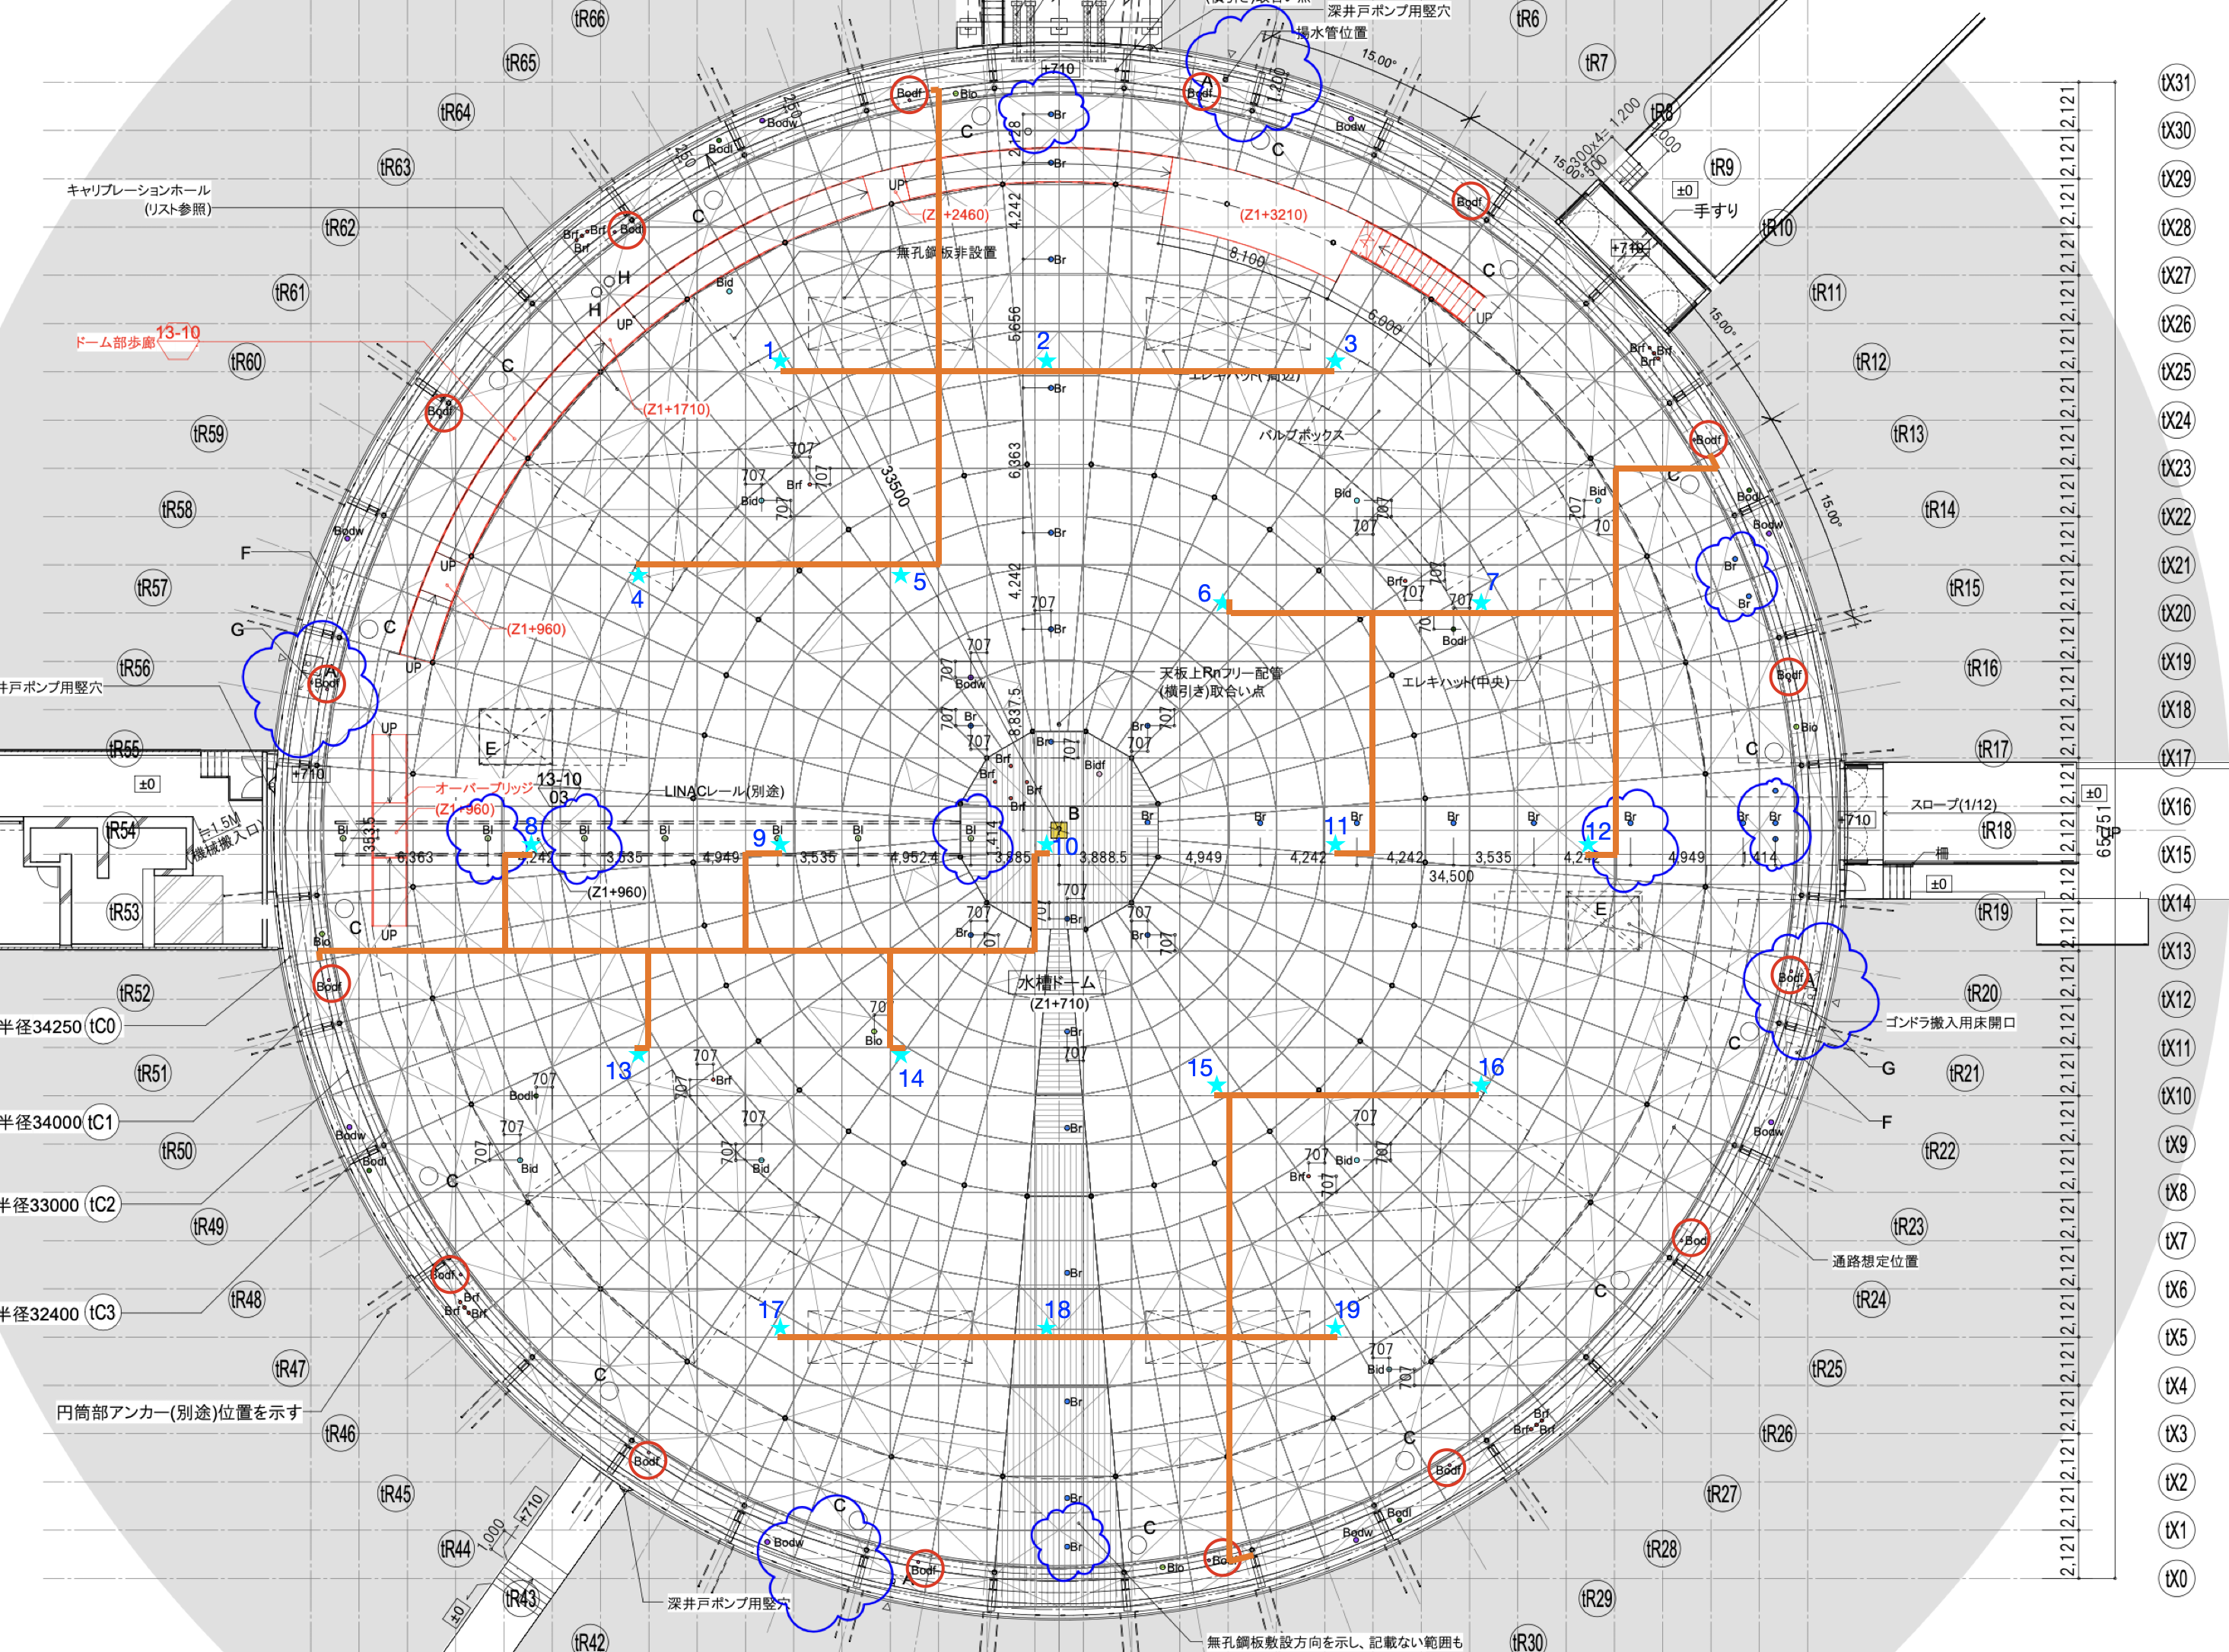
\includegraphics[width=0.9\textwidth]{bottomEndCapMap}
\caption{Map of OD diffuser positions on end-cap (cyan stars), showing fibre routing plan specifically for the bottom end-cap. Schematic shown is for the deck so port positions do not apply, but diffuser positions are the same on top and bottom.}\label{fig:bottomEndCap}
\end{figure}
The proposed fibre routing map for the bottom end-cap OD diffusers is shown in \cref{fig:bottomEndCap}. This involves having connectors at the bottom of verticals tR12, 33, 52 and 65, and thus will utilise ports ODF 3, 8, 12 and 16 for the barrel segments of these fibres, respectively. From the connector, the end-cap portion of the fibre will be routed to the ID side of the support structure, at the closest point where the orthogonal bars shown in \cref{fig:bottomEndCap} meet it. The fibres must then follow this orthogonal path to reach the injectors. Required fibre lengths are measured simply by counting the unit lengths they must traverse, where the $3\times 3$ cell size defines $1u=2121$~mm. These lengths are given in \cref{tab:bottomEndCapLen} for each OD end-cap bottom (ODEB) diffuser.
\begin{table}[h!]
\centering
\begin{tabular}[t]{ccc}\toprule
ODEB	&	Vertical	&	Distance [$u$]	\\ \midrule
1		&		65		&	10		\\
2		&		65		&	9		\\
3		&		65		&	15		\\
4		&		65		&	17		\\
5		&		65		&	11		\\
6		&		12		&	15		\\
7		&		12		&	9		\\
8		&		52		&	8		\\
9		&		52		&	13		\\
10		&		52		&	18		\\	\bottomrule
\end{tabular}
\hspace{1cm}
\begin{tabular}[t]{ccc}\toprule
ODEB	&	Vertical	&	Distance [$u$]	\\ \midrule
11		&		12		&	17		\\
12		&		12		&	12		\\
13		&		52		&	10		\\
14		&		52		&	15		\\
15		&		33		&	12		\\
16		&		33		&	17		\\
17		&		33		&	16		\\
18		&		33		&	10		\\
19		&		33		&	9		\\	\bottomrule
\end{tabular}
\caption{Required distance of fibre optic cable to reach each OD end-cap bottom (ODEB) diffuser, in units of 2121~mm. Also shown is the vertical support that the fibre will be routed from the bottom of.}\label{tab:bottomEndCapLen}
\end{table}
As would be expected, the greatest length of fibre is needed to reach the diffuser position in the centre, ODEB10. This needs a distance of $18u = 38178$~mm. In order to simplify things, this is rounded to 42~m, matching the lengths needed for the deck fibres described in \cref{sec:lengths:sub:len:sub:deck}. All of these OD diffuser fibres will need to have an FC/PC connector on one end, and polished bare fibre on the other.

Not shown here are the ID injector positions. Each of the four sets will be positioned in one of the four $3\times 3$ cell squares diagonally adjacent to the central square. The longest fibre for these is required to run from vertical tR33 to the top right injector, measuring a length of $19u=40299$~mm. This is still below the decided 42~m length, so causes no issues. {\bf Exact cell location will be updated once we have a decided system}. These fibres will require FC/PC connectors on both ends.



\subsubsection{Top end-cap}\label{sec:lengths:sub:len:sub:top}

As previously mentioned, the ID injectors for the top end-cap will be deployed through the Bidf calibration port, meaning that they can be easily removed and replaced should the need arise. In this case, only one section of fibre is needed to go from the injectors to the calibration rack. The length of these is chosen as 10~m, well above the 4506~mm height of the described port. Both ends of these fibres will require FC/PC connectors on. This also matches to the length chosen for the top OD collimators.

The OD diffusers on the top end-cap (labelled ODET 1--19) will be installed in exactly the same $x$ and $y$ locations as for the bottom end-cap. The difference is in the fibre routing, as there is no easy way to get the fibres from an OD fibre port back up to the top end-cap frame. Instead, all of these fibres will also be routed through the Bidf calibration port, and then spread out from this position to each respective diffuser. The fibre routing map for this is given in \cref{fig:topEndCap}.
\begin{figure}[h]
\centering
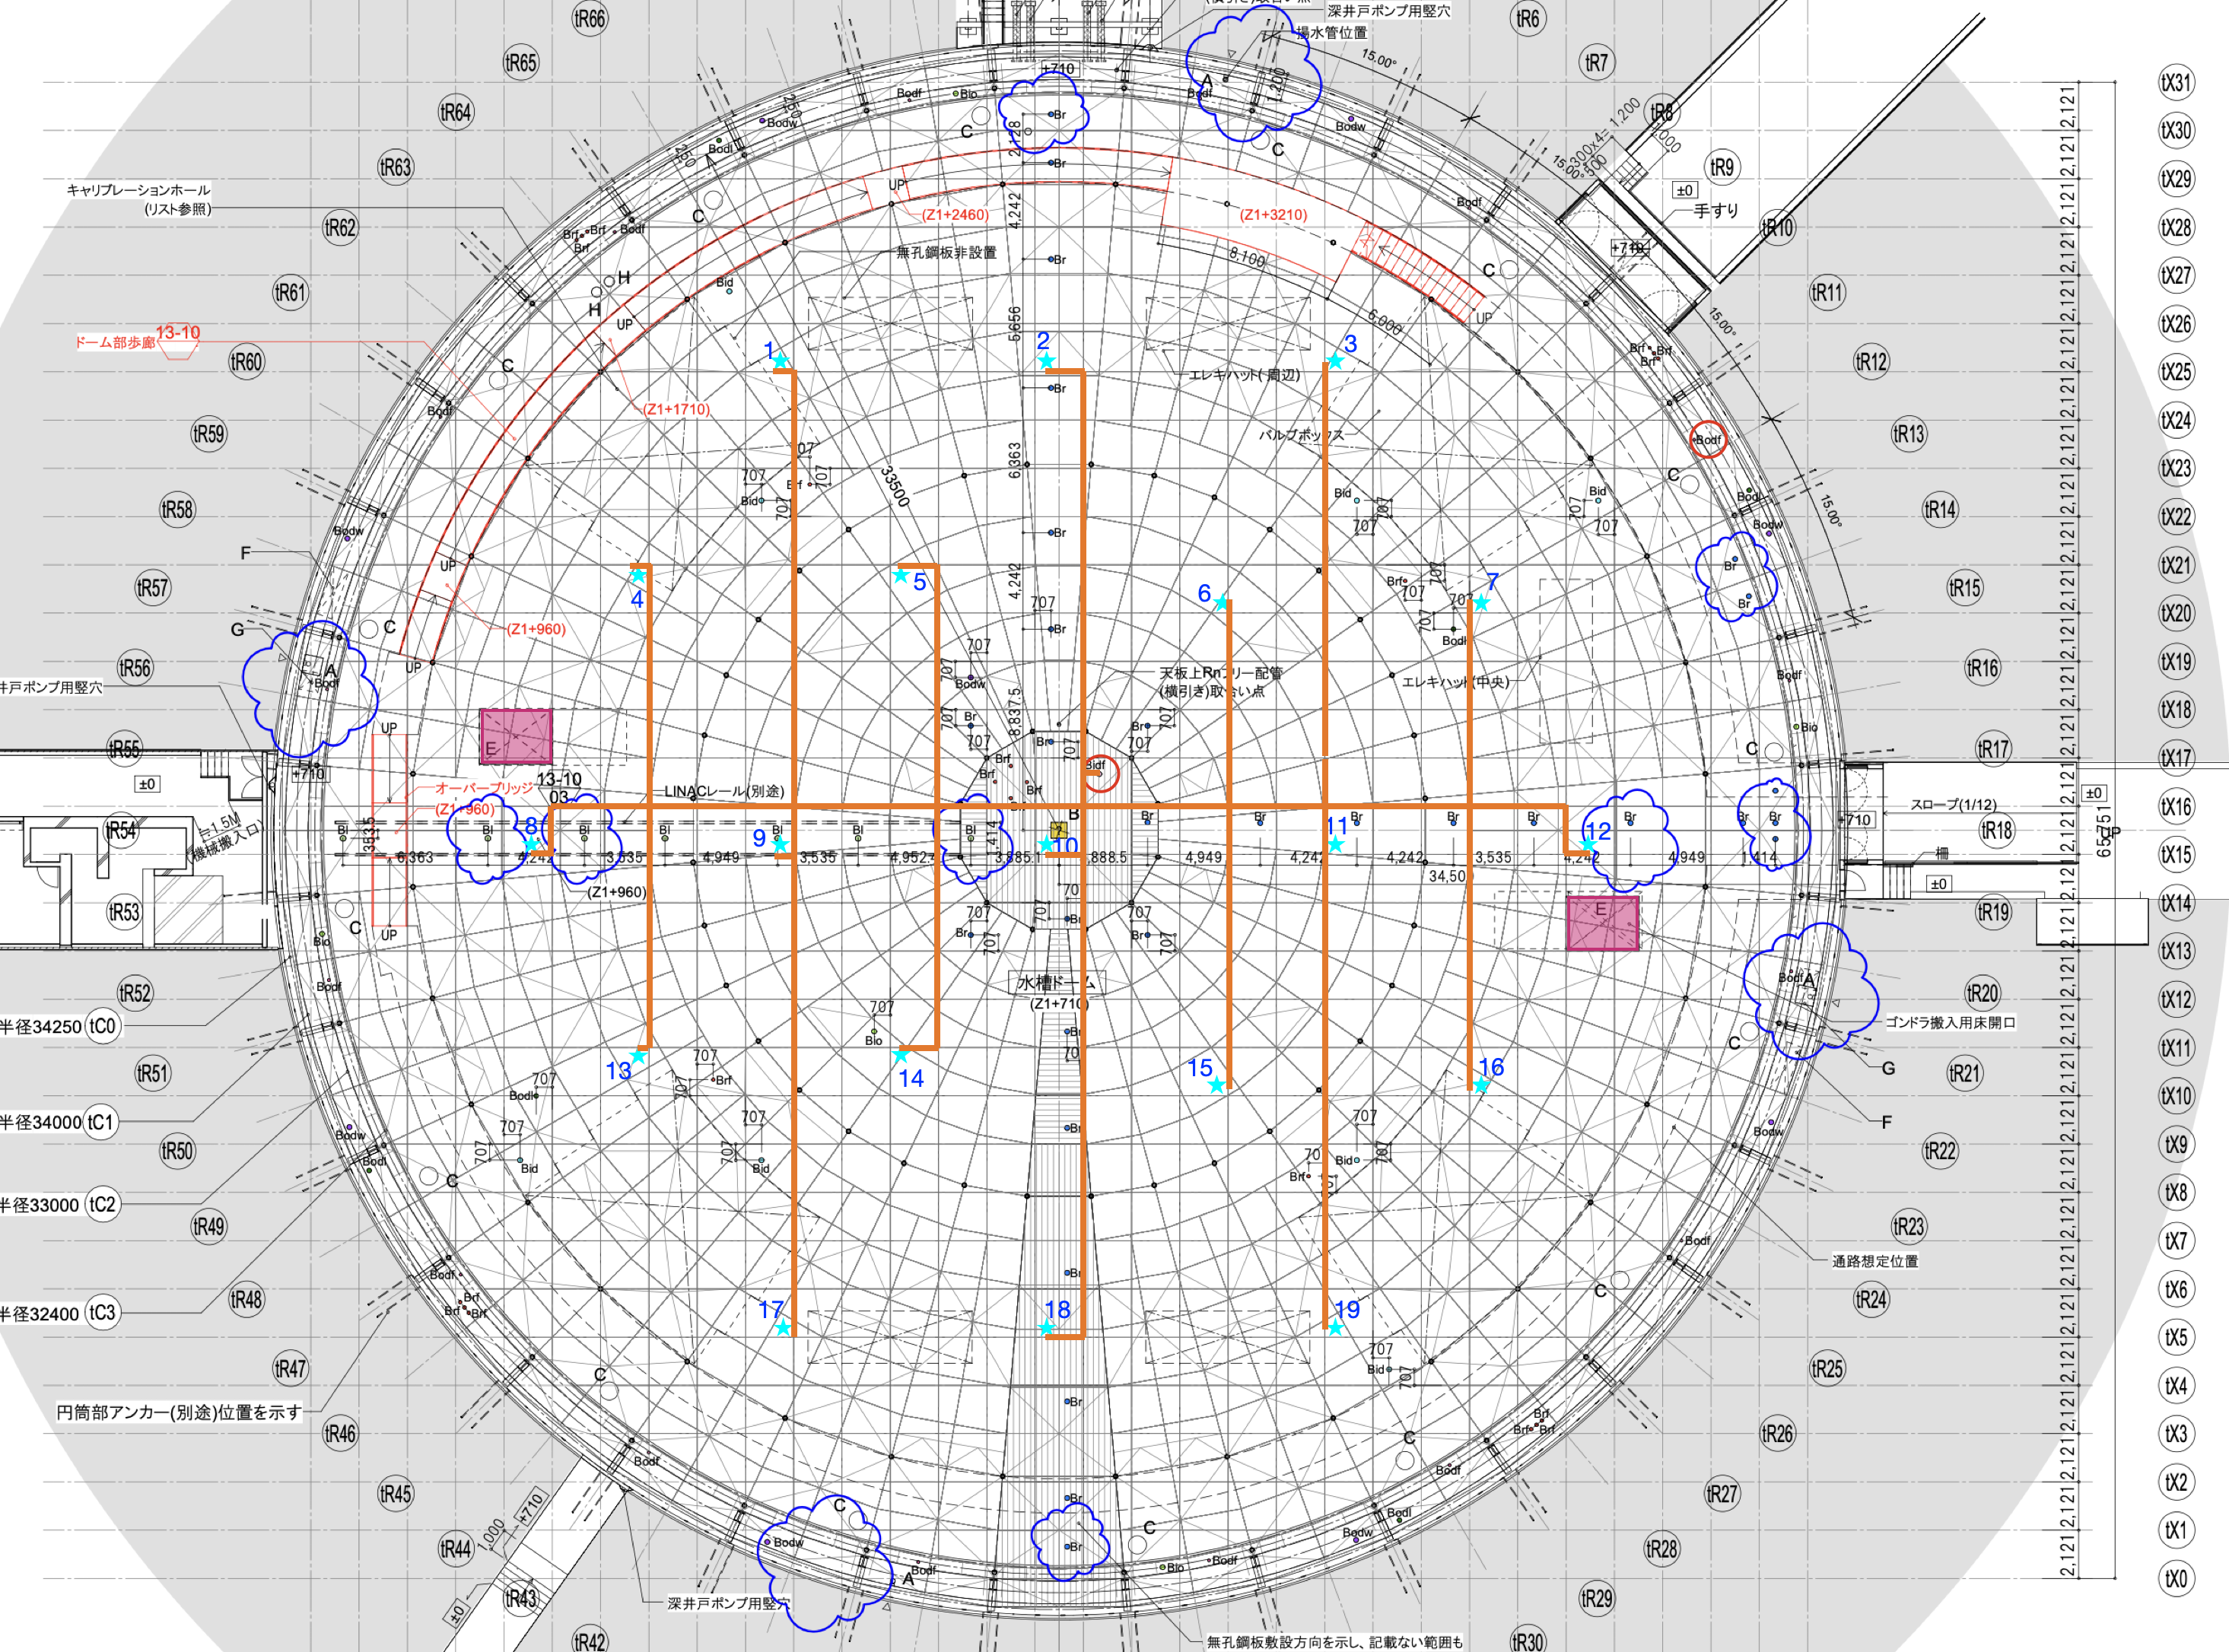
\includegraphics[width=0.9\textwidth]{topEndCapMap}
\caption{Map of OD diffuser positions on end-cap (cyan stars), showing fibre routing plan specifically for the top end-cap. All fibres will be deployed through the Bidf calibration port.}\label{fig:topEndCap}
\end{figure}
In a similar way to \cref{sec:lengths:sub:len:sub:bottom}, the required lengths for these fibres are measured simply by counting the unit lengths along each path. The fibre lengths needed for each injector are given in \cref{tab:topEndCapLen}.
\begin{table}[h!]
\centering
\begin{tabular}[t]{cc}\toprule
ODET	&		Distance [$u$]	\\ \midrule
1		&		18		\\
2		&		10		\\
3		&		17		\\
4		&		17		\\
5		&		11		\\
6		&		10		\\
7		&		15		\\
8		&		15		\\
9		&		10		\\
10		&		4		\\	\bottomrule
\end{tabular}
\hspace{1cm}
\begin{tabular}[t]{cc}\toprule
ODEB	&		Distance [$u$]	\\ \midrule
11		&		8		\\
12		&		14		\\
13		&		17		\\
14		&		11		\\
15		&		11		\\
16		&		16		\\
17		&		19		\\
18		&		14		\\
19		&		18		\\	\bottomrule
\end{tabular}
\caption{Required distance of fibre optic cable to reach each OD end-cap top (ODET) diffuser, in units of 2121~mm.}\label{tab:topEndCapLen}
\end{table}
The greatest length of fibre required comes from connecting to ODET17, the furthest injector from the calibration port. This requires 19 units of length, equating to 40299~mm. Adding on 4506~mm for the height of the calibration port, and then 3000~mm for travel to the electronics rack, a maximum requirement of 47805~mm is obtained. The length of these fibres is therefore rounded to 50~m for contingency. As with the other fibres connecting directly to the OD diffusers, these will need to have FC/PC connectors on one end, and a polished bare fibre on the other. It should be noted that installation of injectors and fibres on the top end-cap is planned to be carried out by company workers rather than researchers, due to additional complications foreseen in this work.


\subsubsection{Patch Fibres}\DIFaddbegin \label{sec:lengths:sub:len:sub:patch}
\DIFaddend 

Along with the long lengths of fibres described in the previous sections, a large number of patch fibres will be required at various points within laser and LED systems.

As described in \cref{sec:lengths:sub:len:sub:barrel}, to connect to all ID injectors bar the top end-cap ones an additional patch fibre is also required. ID injectors will be installed on the PMT support structure during construction, while the fibre installation will be carried out after construction of the structure has been completed, by utilising the OD gondola. In order to avoid workers having to reach far out of the gondola, through the support structure, to attach fibres to the injector housing, short patch fibres will be attached to the injectors at the time of their installation. These will span the dead region and be fixed to the outer side of the structure, so that the long fibres can be connected directly to the patch fibres. As part of this a fibre guide will be used, to ensure that the end of the fibre will be pointing vertically upwards for connection, without the fibre being pushed past its bending radius. The required lengths have been measured using a mockup of the support, obtaining values of 640~mm for the diffuser and 530~mm for the collimator. Both ends of these patch fibres will need to have FC/PC connectors.

Based on \cref{fig:laserswitches}, eight patch fibres will be required for within the laser system itself, not including the five that will come coupled to the laser heads. Five of these will run from individual attenuators to connect the laser heads to the 1x8 switch, and then three are used for the connections between the 1x8 and 1x80 switch, which includes integrating the fibre splitter for the monitor PMT. These will all be FG105UCA fibres with FC/PC connectors on either end, with a rough length requirement of \DIFdelbegin \DIFdel{\mbox{%DIFAUXCMD
$\sim50$
}%DIFAUXCMD
}\DIFdelend \DIFaddbegin \DIFadd{\mbox{%DIFAUXCMD
$\sim100$
}%DIFAUXCMD
}\DIFaddend ~cm.

A series of short patch fibres will also be required for the LED system. Each LED pulser board will feature a connector sitting atop the surface mounted LED, with space for two fibres to be inserted. One of these will be directly above the LED to collect as much light as possible, and this will be used for illuminating the OD diffusers. The second will be offset, collecting some of the remaining light to be used as a signal for monitoring purposes. As the monitor system will sit at the electronics rack, much less fibre will be used and therefore less initial light input is required. The design for the the fibre connector is currently ongoing, and will be used to confirm the required length of the patch fibres within the pulser board crates. Initial measurements of the required lengths, which are different due to the topology of the connector, give $21.1\pm1.4$~cm and $18.4\pm0.6$~cm, where the uncertainties here are the measured tolerances on the length. Any shorter than this and the cable will not reach. If the cables are longer, they would be required to bend at a greater angle than their specified bending radius, which will cause degradation over the lifetime of the system. As the connector for the LED pulser board will have the fibres epoxied in, each of these patch cables will require FC/PC connectors on one end, with the other cleaved and polished.

The final set of patch cables for the LED pulser system is that used to connect to the monitor PMTs. The internal patch cable from the LED connector will go into a patch panel on the front of the electronics rack. These patch cables will carry light from that patch panel to a system of several monitor PMTs in the same electronics rack. These will be 1~m long, with an FC/PC connector on the patch panel end, and polished bare fibre at the PMT-facing end.

\cref{tab:fibreSummaryLaser,tab:fibreSummaryLED} summarise all the required fibres for the laser and LED systems respectively, detailing the chosen type, length, connectors and quantities needed. Quantities are also detailed for the cases where the fibres that traverse the barrel region are split into different lengths to minimise excess, which is the preferred approach for this system. \DIFaddbegin \DIFadd{ In these tables, fibres of the same configuration are grouped together. \mbox{%DIFAUXCMD
\cref{tab:fibreDetailsLaser,tab:fibreDetailsLED} }\hskip0pt%DIFAUXCMD
in \mbox{%DIFAUXCMD
\cref{app:fibreconfig} }\hskip0pt%DIFAUXCMD
breaks this down further for additional clarity. As discussed in \mbox{%DIFAUXCMD
\cref{sec:fibre:sub:att:sub:results}}\hskip0pt%DIFAUXCMD
, all fibres with be tubed using the Thorlabs FT030-BK tubing, the same as used for the UKLI system in Super-K. The exception to this is the LED crate fibres, which will instead be colour-coded}\DIFaddend .

\begin{table}[h]
\centering
\setlength{\tabcolsep}{4pt}
\begin{tabular}{ccccc}
\toprule
Length [m]	&	Connector A	&	Connector B	&	Required no.	&	Use		\\ \midrule
76			&	FC/PC		&	FC/PC		&	73				&	Barrel (all)$^\dagger$	\\
42			&	FC/PC		&	FC/PC		&	84				&	Deck and bottom	\\
10			&	FC/PC		&	FC/PC		&	5				&	Top ID inj. and top OD coll. \\
\DIFdelbeginFL \DIFdelFL{0.64		}\DIFdelendFL \DIFaddbeginFL \DIFaddFL{1			}\DIFaddendFL &	FC/PC		&	FC/PC		&	\DIFdelbeginFL \DIFdelFL{32				}\DIFdelendFL \DIFaddbeginFL \DIFaddFL{8				}\DIFaddendFL &	\DIFdelbeginFL \DIFdelFL{ID diffuser }\DIFdelendFL \DIFaddbeginFL \DIFaddFL{Laser system }\DIFaddendFL patch cable \\
\DIFdelbeginFL \DIFdelFL{0.56		}\DIFdelendFL \DIFaddbeginFL \DIFaddFL{0.64		}\DIFaddendFL &	FC/PC		&	FC/PC		&	32				&	ID \DIFdelbeginFL \DIFdelFL{collimator }\DIFdelendFL \DIFaddbeginFL \DIFaddFL{diffuser }\DIFaddendFL patch cable	\\
\DIFdelbeginFL \DIFdelFL{0.5			}\DIFdelendFL \DIFaddbeginFL \DIFaddFL{0.56		}\DIFaddendFL &	FC/PC		&	FC/PC		&	\DIFdelbeginFL \DIFdelFL{8				}\DIFdelendFL \DIFaddbeginFL \DIFaddFL{32				}\DIFaddendFL &	\DIFdelbeginFL \DIFdelFL{Laser system }\DIFdelendFL \DIFaddbeginFL \DIFaddFL{ID collimator }\DIFaddendFL patch cable	\\ \midrule
\multicolumn{3}{l}{$^\dagger$Staged approach:} &					&			\\
32			&	FC/PC		&	FC/PC		&	16				&	Barrel (levels 1+2) \\
58			&	FC/PC		&	FC/PC		&	24				&	Barrel (levels 3+4+5)	\\
76			&	FC/PC		&	FC/PC		&	33				&	Barrel (levels \DIFdelbeginFL \DIFdelFL{5+}\DIFdelendFL 6+\DIFaddbeginFL \DIFaddFL{7+}\DIFaddendFL bottom)	\\
\bottomrule
\end{tabular}
\caption{List of all required fibres for the laser system with necessary lengths, connector configurations, quantities and uses.}\label{tab:fibreSummaryLaser}
\end{table}

\begin{table}[h]
\centering
\setlength{\tabcolsep}{4pt}
\begin{tabular}{ccccc}
\toprule
Length [m]	&	Connector A	&	Connector B	&	Required no.	&	Use		\\ \midrule
76			&	FC/PC		&	FC/PC		&	19				&	Barrel to bottom	\\
76			&	FC/PC		&	Bare		&	84				&	Barrel injs (all)$^\dagger$	\\
50			&	FC/PC		&	Bare		&	19				&	Top diffusers \\
42			&	FC/PC		&	FC/PC		&	103				&	Deck		\\
42			&	FC/PC		&	Bare		&	19				&	Bottom diffusers	\\
1			&	FC/PC		&	Bare		&	122				&	Crate to monitor PMT(s)	\\
0.21		&	FC/PC		&	Bare		&	122				&	Crate internal patch 1	\\
0.18		&	FC/PC		&	Bare		&	122				&	Crate internal patch 2 \\ \midrule\multicolumn{3}{l}{$^\dagger$Staged approach:}&					&			\\
32			&	FC/PC		&	Bare		&	24				&	Barrel (levels 1+2) \\
58			&	FC/PC		&	Bare		&	36				&	Barrel (levels 3+4+5)	\\
76			&	FC/PC		&	Bare		&	24				&	Barrel (levels \DIFdelbeginFL \DIFdelFL{5+}\DIFdelendFL 6\DIFaddbeginFL \DIFaddFL{+7}\DIFaddendFL )	\\
\bottomrule
\end{tabular}
\caption{List of all required fibres for the LED system with necessary lengths, connector configurations, quantities and uses.}\label{tab:fibreSummaryLED}
\end{table}



\clearpage

\section{Photon Yield Requirements}\label{sec:photonreq}

With a series of points in the system where light can be lost, it is important to verify the number of photons required to be injected into the tank for calibration, and the initial laser power required to achieve this. This section describes the study performed to calculate these required numbers.

A series of simulations were run using the Monte Carlo generation package for Hyper-K, WCSim \cite{bib:wcsim}, using diffusers at each vertical depth level (injector indices 0, 4, 8, 12, 16, 20, 24), along with one on the top end cap (28) and one on the bottom (32). For each injector, sets of simulations were run with injected light at wavelengths of 365~nm, 395~nm, 415~nm, 465~nm, 496~nm and 525~nm. These are a subset of the wavelengths used for attenuation measurements in \cref{sec:fibre:sub:att:sub:method} and, although not necessarily the exact wavelengths that will be used in the system, allow for explicit calculation of loss factors due to attenuation without interpolating between measurements. Within each of these sets, a number of simulations were run at differing values of injected photons, initially increasing in steps of 200, before moving to larger steps for the higher wavelengths which required greater numbers. For all simulations, 1000 events are run, using nominal water parameters. The injector is treated as an ideal diffuser, with a 40\degree\ opening half-angle, and dark noise was disabled.

The aim for general running of the diffusers is 1\% PMT coverage within the diffuser spot, and so this is used as the target for these studies. For each of the 1000 events in a simulation, the number of hit PMTs within the diffuser spot is calculated and histogrammed. This is fit with a Gaussian distribution, and the mean of that taken to be the number of hit PMTs within the spot. An example of this distribution is shown in \cref{fig:nhits_dif0_365_1000ph_plot}.
\begin{figure}[h]
\centering
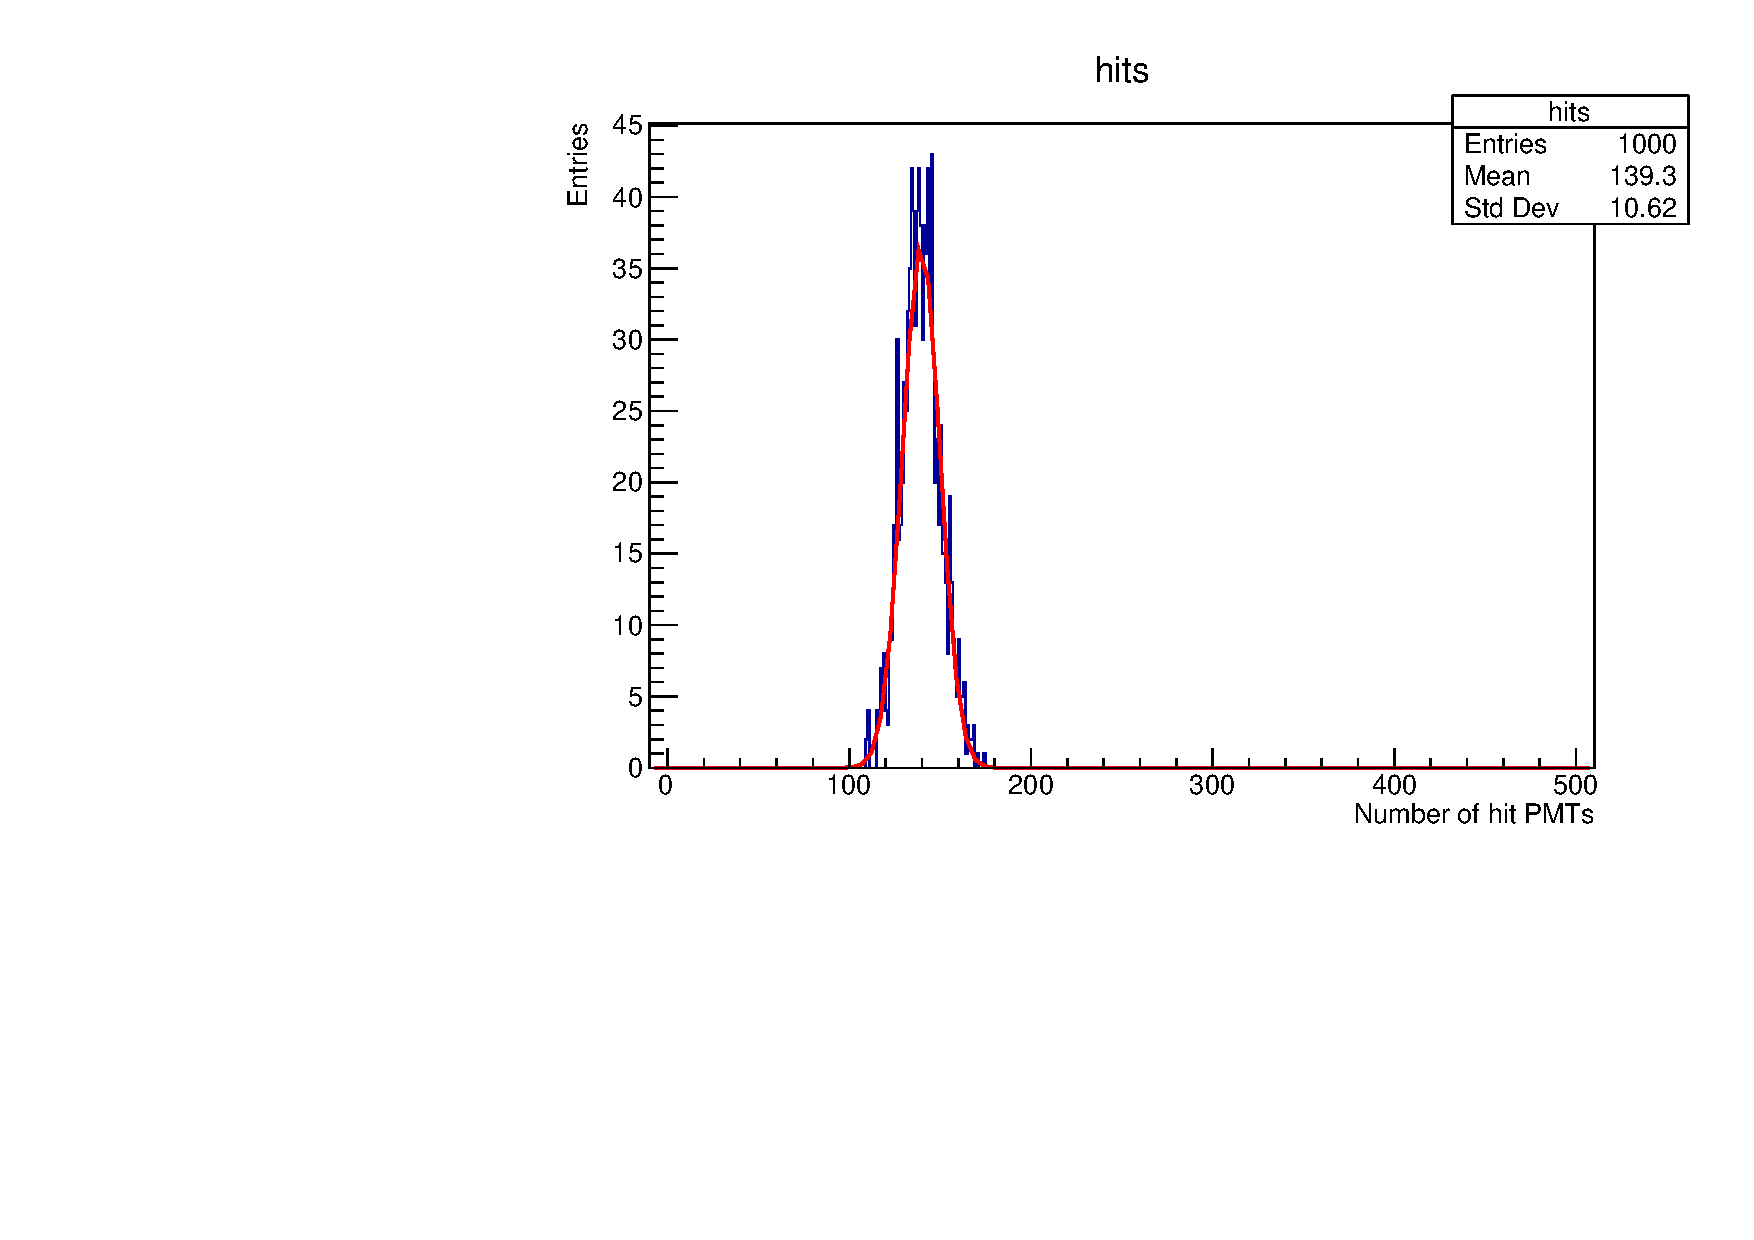
\includegraphics[width=0.7\textwidth]{nhits_dif0_365_1000ph_plot.pdf}
\caption{Number of hit PMTs in the spot of diffuser 0, for 1000 injected photons at a wavelength of 365~nm.}\label{fig:nhits_dif0_365_1000ph_plot}
\end{figure}
The obtained mean can then be compared to the total number of PMTs within the diffuser spot, to calculate the percentage coverage. This is repeated for all simulations, and compared to the 1\% requirement for all injectors to obtain the minimum number of injected photons required.

The coverage percentages for all nine injectors for the 365~nm wavelength are given in \cref{fig:coverage_365}.
\begin{figure}
\centering
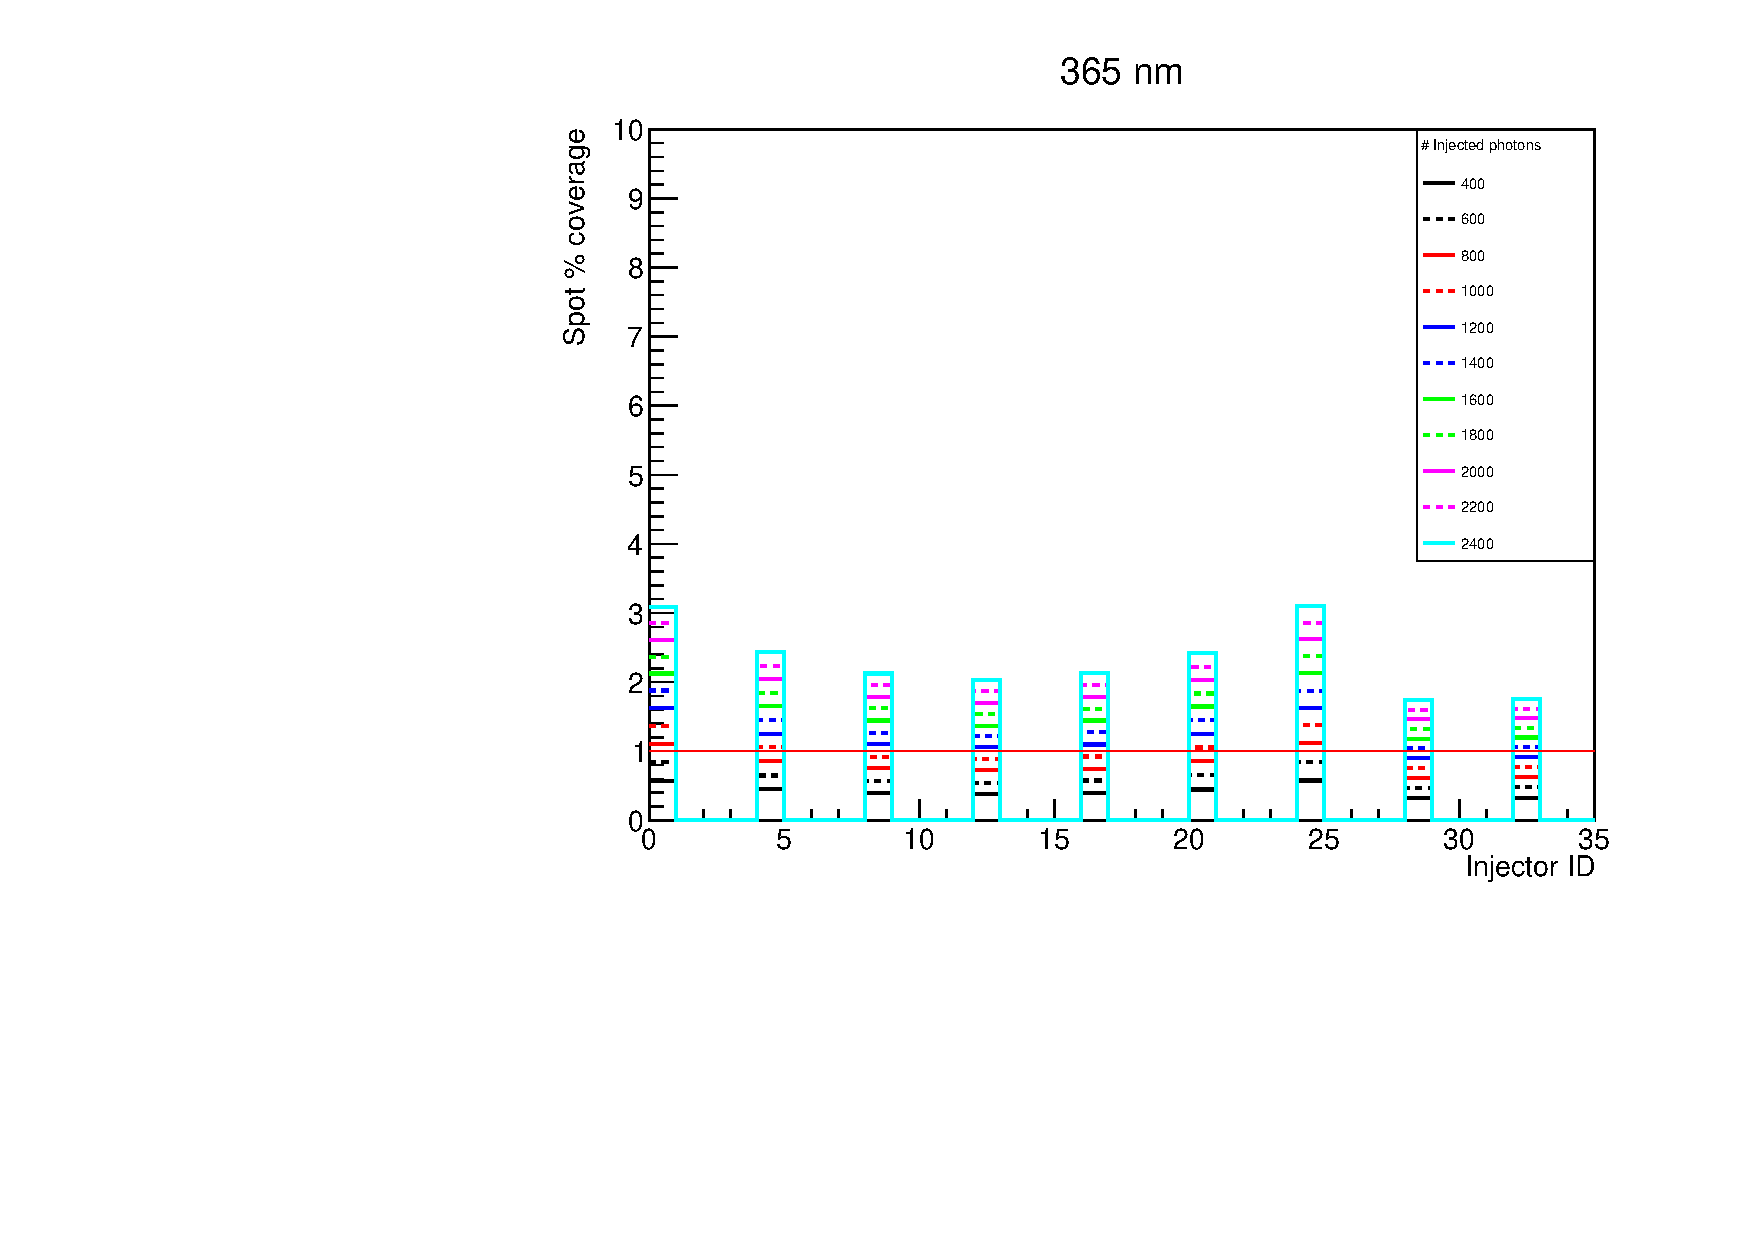
\includegraphics[width=0.8\textwidth]{coverage_365.pdf}
\caption{Coverage percentages as a function of diffuser position, for differing numbers of injected photons of 365~nm wavelength. The 1\% level is shown by the red line.}\label{fig:coverage_365}
\end{figure}
The shape of these plots can be understood by thinking about the geometry of the detector. Injectors 0 and 24 are the barrel injectors closest to the bottom and top endcaps respectively, so those diffusers illuminate a large part of the respective end caps. The shorter path lengths between these injectors and the endcaps results in a greater amount of the initial photons causing hits, and therefore less required for 1\% coverage. As the injector positions move towards the middle, there is less to no overlap with the end caps, increasing the average path length to PMTs. The final two injectors, those on the top and bottom end caps, have the greatest distance to the opposite side of the tank. There are therefore more PMTs are in the spot, and with the greater distance photons are required to travel, means a greater number of injected photons are needed for 1\% coverage. At this wavelength, 1400 injected photons are required to obtain at least 1\% coverage in all injectors. The behaviour described repeats for all wavelengths checked, making the top and bottom injectors the limiting cases for each.

The approximate number of photons required to achieve 1\% spot coverage per wavelength is given in \cref{tab:coverage}. These numbers can then be used to calculate the required laser power per wavelength, accounting for loss due to attenuation in the fibres and other points of inefficiency within the system.
\begin{table}[h]
\centering
\begin{tabular}{cc}
\toprule
Wavelength (nm) & N photons for 1\% coverage \\ \midrule
365 & 1400 \\
395 & 1200 \\
415 & 2000 \\
465 & 3000 \\
496 & 6000 \\
525 & 24000\\ \bottomrule
\end{tabular}
\caption{Approximate number of injected photons required for 1\% diffuser spot coverage, per wavelength.}\label{tab:coverage}
\end{table}
The attenuation coefficients calculated in \cref{sec:fibre:sub:att:sub:method} for the above wavelengths are used to obtain the attenuation factors for the fibres, assuming the 175~m calculated in \cref{sec:lengths}. The fibre is assumed to be the Thorlabs FG105UCA favoured in \cref{sec:fibre:sub:choice}.

Additional light loss factors are also added into the calculations. A 90\% loss is included to account for the efficiency of the ID diffuser. To account for losses in the fibre switch, we use the worst case scenario from the Weinert FP400URT measurements, and assume a 25\% loss at each stage of the switch. As any larger switch is formed by daisy-chaining 1x4 switches, this 25\% loss can be experienced up to 6 times (twice for a 1x8 switch plus four times for a 1x80 switch), resulting in an efficiency of $0.75^6 \simeq 0.18$. As the Weinert GIF50C results showed much greater transmission these numbers are considered conservative, and the final efficiency of the device will depend on the internal fibre used. Finally, a factor of 50\% is included to account for any losses in coupling fibres together across the system.

Applying these scaling factors to the requirements in \cref{tab:coverage} yields the required number of photons per pulse from the laser, which goes up to at most $2.4\times10^5$ at 525~nm. This can easily be translated to the required energy per pulse, which is given in \cref{fig:laserenergy}.
\begin{figure}
\centering
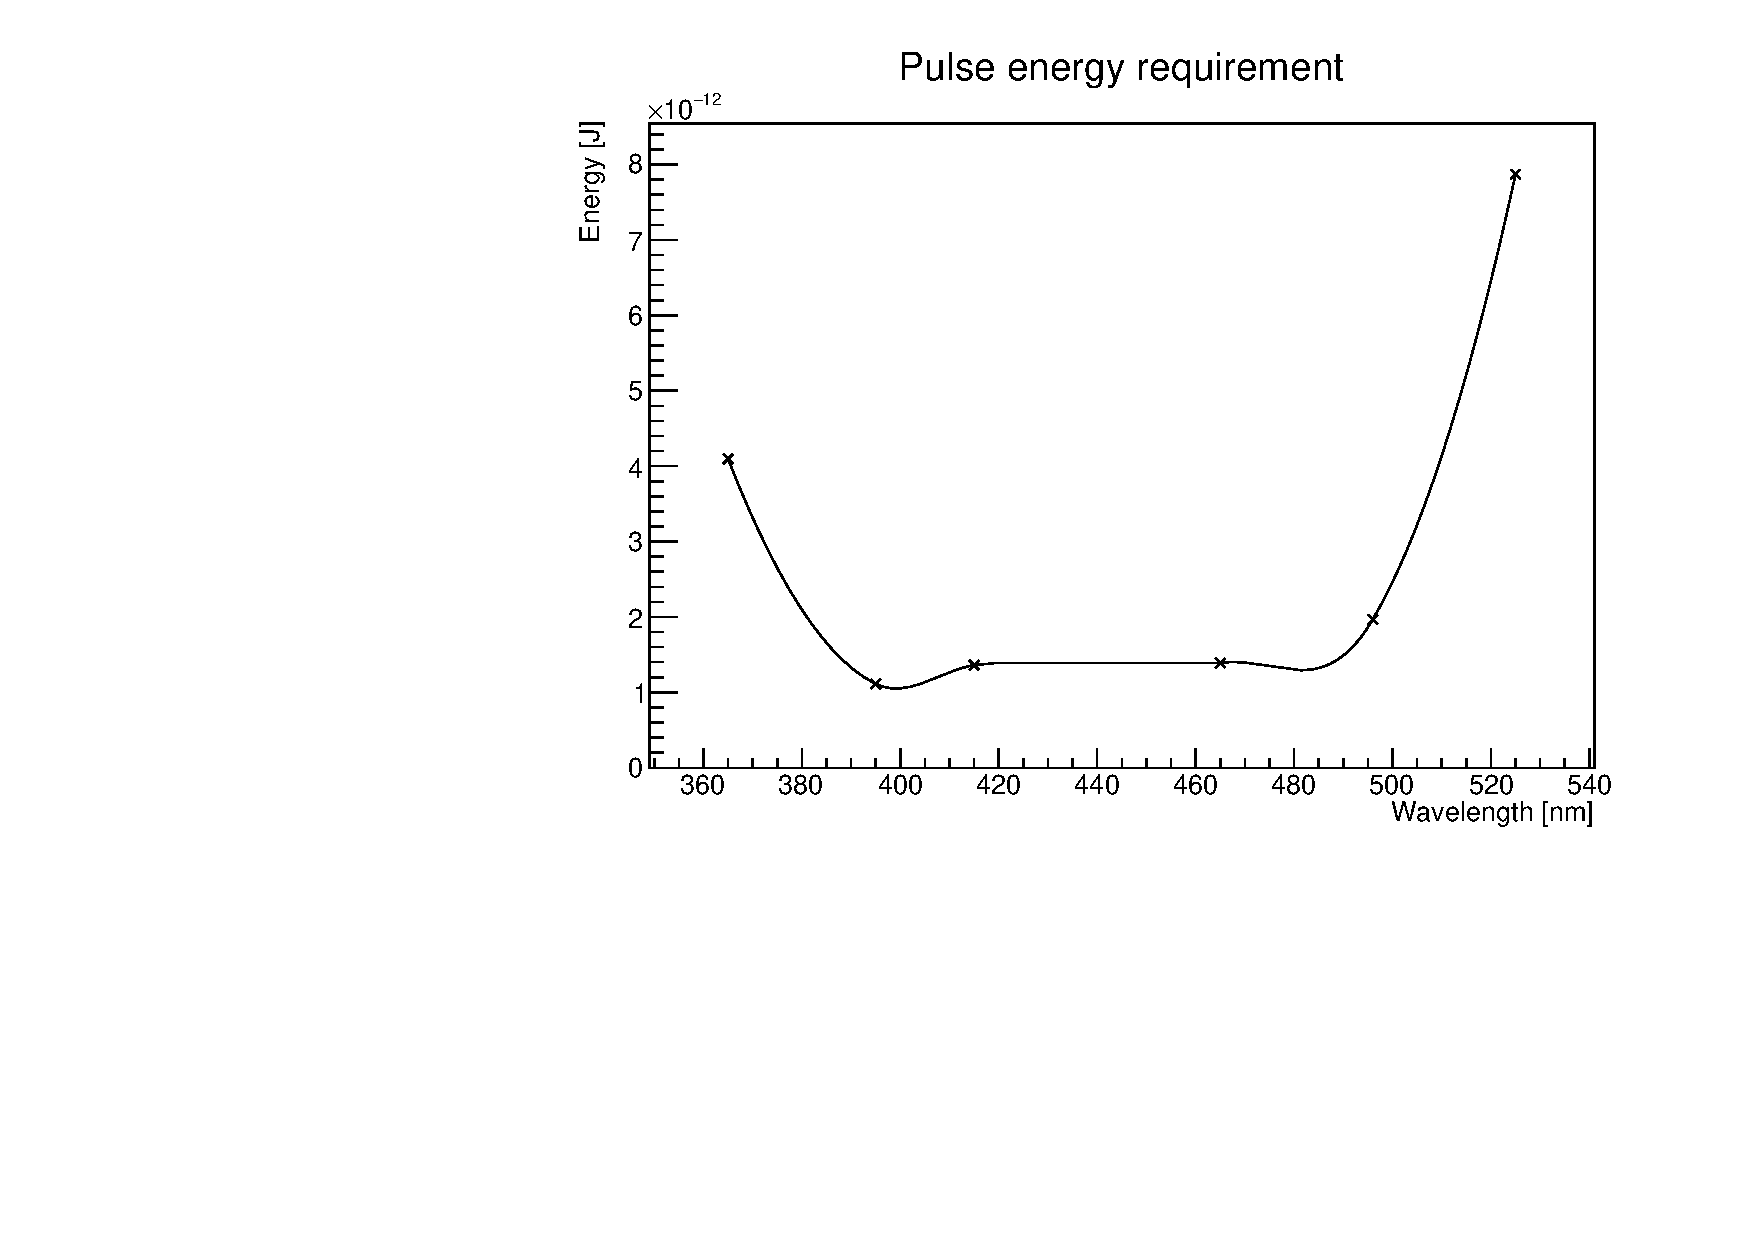
\includegraphics[width=0.7\textwidth]{pulseEnergyReq.pdf}
\caption{Laser pulse energy as a function of wavelength required to achieve 1\% diffuser spot coverage.}\label{fig:laserenergy}
\end{figure}
Finally, assuming a 1~kHz pulse frequency for occasional intensive calibration runs, the average power required of the lasers at each wavelength is given in \cref{fig:laserpower}.
\begin{figure}
\centering
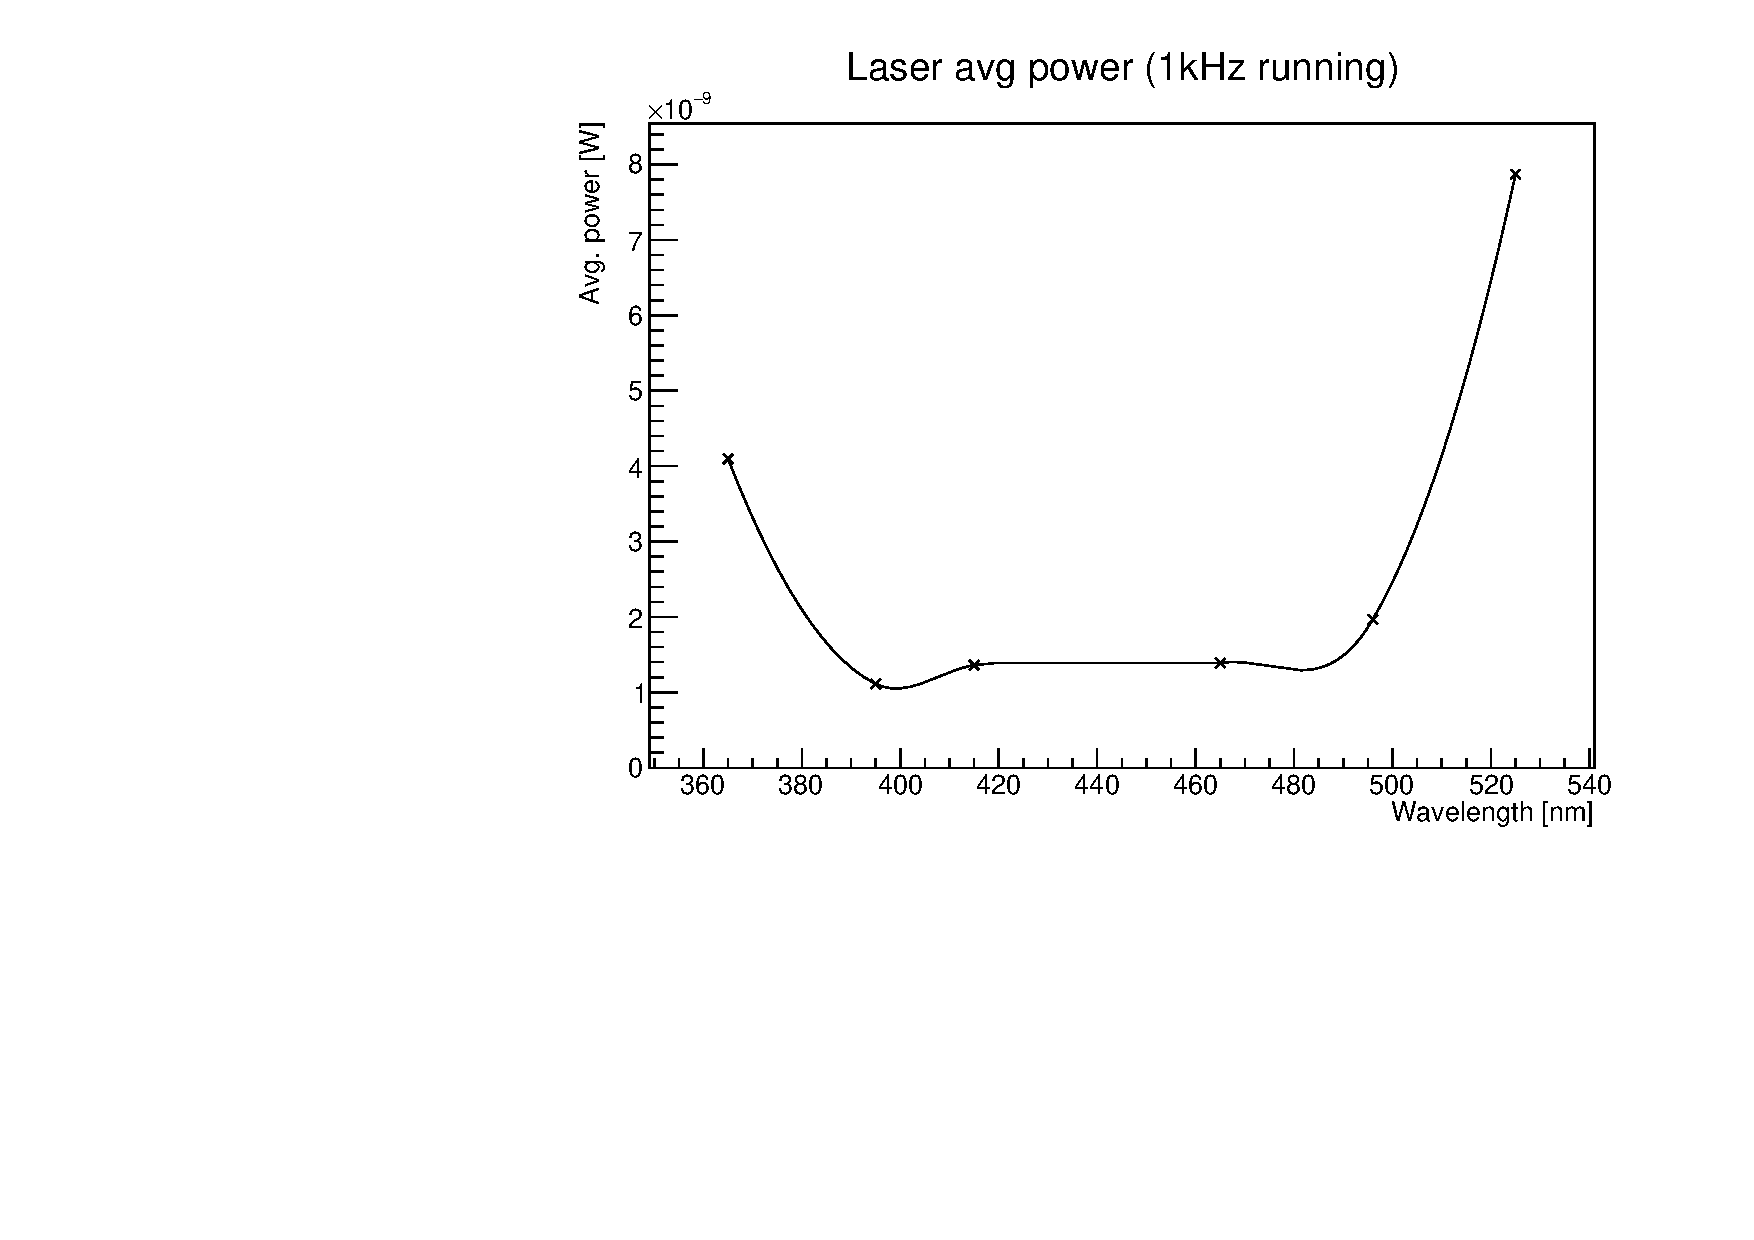
\includegraphics[width=0.7\textwidth]{avgPowerReq.pdf}
\caption{Laser average power as a function of wavelength required to achieve 1\% diffuser spot coverage, for 1~kHz running.}\label{fig:laserpower}
\end{figure}



\section{Summary}
This technical note describes the tests performed on candidate fibre optic cables, which are used to justify the choices made for optimal fibres to use for the ID and OD systems. For the ID system, along with the OD collimators, Thorlabs FG105UCA is chosen. This fibre showed the least attenuation of the four types tested, in the UV wavelength range which is of most interest, and also matches the fibre type that has already been chosen as the internal feed-through for the optics themselves. This reduces losses that would otherwise be obtained when coupling fibres of different types together. This is the reason for choosing this fibre, despite the fact it exhibits a greater increase in pulse rise time than the other candidates. A high frequency read-out system is currently in development in order to make complete measurements of the dispersion from the full lengths of this fibre, as this is still an important property to understand.

For the OD diffuser system, the fibre if choice is instead Thorlabs FP400URT. While this showed increased attenuation at lower wavelengths when compared to FG105UCA, the advantage of the former fibre type is the diameter being four times greater. This makes coupling an LED to the fibre considerably easier, and ensures a greater amount of light is directed into the fibre in the first place.

A series of measurements of 1x4 fibre switching devices have also been presented, manufactured by two different companies. The results for power transmission found the Weinert device with GIF50C internal fibre to be the best, while for power variation the Agiltron FP400URT device performed slightly better than the others. However, when making power measurements, none-zero power measurements were observed on channels of the Agiltron device that were not being illuminated. Dedicated measurements of this showed cross talk between several different channels on the Agiltron device, whereas no measurable cross talk was found for either of the Weinert devices. Coupled with the fact the support from Weinert was vastly superior, which will be incredibly important for maintaining the device over the lifetime of the experiment, the favoured company is Weinert. The internal fibre will be the same as that used for the ID laser system, and as such should be FG105UCA, as discussed already.

\newpage
\begin{thebibliography}{99}

%%diffuser TN
\bibitem{bib:tn0042}
S. Boyd {\it et al.}, Hyper-Kamiokande Light Injector Diffuser Technical Note (HK-TN-0042)

%%collimator TN
\bibitem{bib:tn0065}
S. Boyd {\it et al.}, Hyper-Kamiokande Light Injector Collimator Technical Note (HK-TN-0065)

%%laser specs
\bibitem{bib:picoquant}
PicoQuant GmbH, PicoQuant, \url{https://www.picoquant.com}

\bibitem{bib:laserdriver}
PicoQuant GmbH, Sepia PDL 828 Multichannel Picosecond Diode Laser Driver, September 2021, \url{https://www.picoquant.com/images/uploads/downloads/7920-sepia_pdl828.pdf}

\bibitem{bib:laserhead}
PicoQuant GmbH, LDH Series Picosecond Laser Diode Heads for PDL 800-D/PDL 828, January 2024, \url{https://www.picoquant.com/images/uploads/downloads/datasheet_ldh_series.pdf}

\bibitem{bib:LDH}
PicoQuant GmbH, LDH-FA Series Amplified Picosecond Pulsed Laser Diode Heads, September 2022, \url{https://www.picoquant.com/images/uploads/downloads/18-ldh-fa-series_3.pdf}

%%fibres
\bibitem{bib:fp200urt}
Thorlabs Inc., FP200URT Specifications, 6th February 2024, \DIFdelbegin %DIFDELCMD < \url{https://www.thorlabs.com/drawings/d13a8cb83b2fa5fc-1B09855E-D596-03E0-87CB959C07E1E119/FP200URT-SpecSheet.pdf}
%DIFDELCMD < %%%
\DIFdelend \DIFaddbegin \url{https://www.thorlabs.com/thorproduct.cfm?partnumber=FP200URT}
\DIFaddend 

\bibitem{bib:fp400urt}
Thorlabs Inc., FP400URT Specifications, 6th December 2022, \DIFdelbegin %DIFDELCMD < \url{https://www.thorlabs.com/drawings/d13a8cb83b2fa5fc-1B09855E-D596-03E0-87CB959C07E1E119/FP400URT-SpecSheet.pdf}
%DIFDELCMD < %%%
\DIFdelend \DIFaddbegin \url{https://www.thorlabs.com/thorproduct.cfm?partnumber=FP400URT}
\DIFaddend 

\bibitem{bib:fg050uga}
Thorlabs Inc., FG050UGA Specifications, 22nd April 2024, \DIFdelbegin %DIFDELCMD < \url{https://www.thorlabs.com/drawings/d13a8cb83b2fa5fc-1B09855E-D596-03E0-87CB959C07E1E119/FG050UGA-SpecSheet.pdf}
%DIFDELCMD < %%%
\DIFdelend \DIFaddbegin \url{https://www.thorlabs.com/thorproduct.cfm?partnumber=FG050UGA}
\DIFaddend 

\bibitem{bib:fg105uca}
Thorlabs Inc., FG105UCA Specifications, 22nd April 2024, \DIFdelbegin %DIFDELCMD < \url{https://www.thorlabs.com/drawings/d13a8cb83b2fa5fc-1B09855E-D596-03E0-87CB959C07E1E119/FG105UCA-SpecSheet.pdf}
%DIFDELCMD < %%%
\DIFdelend \DIFaddbegin \url{https://www.thorlabs.com/thorproduct.cfm?partnumber=FG105UCA}
\DIFaddend 

\bibitem{bib:gif50c}
Thorlabs Inc., GIF50C Specifications, 6th February 2024, \DIFdelbegin %DIFDELCMD < \url{hhttps://www.thorlabs.com/drawings/d13a8cb83b2fa5fc-1B09855E-D596-03E0-87CB959C07E1E119/GIF50C-SpecSheet.pdf}
%DIFDELCMD < %%%
\DIFdelend \DIFaddbegin \url{https://www.thorlabs.com/thorproduct.cfm?partnumber=GIF50C}
\DIFaddend 

\bibitem{bib:gif50d}
Thorlabs Inc., GIF50D Specifications, 6th February 2024, \DIFdelbegin %DIFDELCMD < \url{https://www.thorlabs.com/drawings/d13a8cb83b2fa5fc-1B09855E-D596-03E0-87CB959C07E1E119/GIF50D-SpecSheet.pdf}
%DIFDELCMD < %%%
\DIFdelend \DIFaddbegin \url{https://www.thorlabs.com/thorproduct.cfm?partnumber=GIF50D}
\DIFaddend 


\bibitem{bib:opm}
Thorlabs Inc., Optical Power Meter PM100USB Operation Manual v1.7, 28th March 2023, \DIFdelbegin %DIFDELCMD < \url{https://www.thorlabs.com/drawings/358f9a4c347897ec-F6D46DF6-F3B1-0FC2-1D78C79FC5065F04/PM100USB-Manual.pdf}
%DIFDELCMD < %%%
\DIFdelend \DIFaddbegin \url{https://www.thorlabs.com/thorproduct.cfm?partnumber=pm100usb}
\DIFaddend 

\bibitem{bib:opmsensor}
Thorlabs Inc., Fiber Power Head with Silicon Detector S150C, 4th February 2016, \DIFdelbegin %DIFDELCMD < \url{https://www.thorlabs.com/drawings/d13a8cb83b2fa5fc-1B09855E-D596-03E0-87CB959C07E1E119/S150C-SpecSheet.pdf}
%DIFDELCMD < %%%
\DIFdelend \DIFaddbegin \url{https://www.thorlabs.com/thorproduct.cfm?partnumber=S150C}
\DIFaddend 

\bibitem{bib:hpmt}
Hamamatsu Photonics K.K., Photomultiplier Tube Modules H10720/H10721 Series, September 2024, \url{https://www.hamamatsu.com/content/dam/hamamatsu-photonics/sites/documents/99_SALES_LIBRARY/etd/H10720_H10721_TPMO1062E.pdf}

\bibitem{bib:scope}
Tektronix Inc., 5 Series MSO Mixed Signal Oscilloscope Datasheet, \url{https://www.tek.com/en/datasheet/5-series-mso}

\bibitem{bib:hkpmt}
Y. Nishimura, The Box-and-Line PMT (R12860), (HK-TN-0009 Ver.1.2 RevId20200718)

\bibitem{bib:matingsleeve}
Thorlabs Inc., ADAFC1 - FC/PC to FC/PC Mating Sleeve, Wide Key (2.2 mm), D-Hole, \DIFdelbegin %DIFDELCMD < \url{https://www.thorlabs.com/drawings/2a489cabfd9515d-9C4A02B3-EAE7-54D1-C7D705D1F6B147AD/ADAFC1-SpecSheet.pdf}
%DIFDELCMD < %%%
\DIFdelend \DIFaddbegin \url{https://www.thorlabs.com/thorproduct.cfm?partnumber=adafc1}
\DIFaddend 

\DIFaddbegin \bibitem{bib:ft030bk}
\DIFadd{Thorlabs Inc., FT030-BK - Black Reinforced Ø3 mm Furcation Tubing, }\url{https://www.thorlabs.com/thorproduct.cfm?partnumber=FT030-BK}

\DIFaddend \bibitem{bib:skgd2}
K. Abe {\it et al.}, Second gadolinium loading to Super-Kamiokande, NIM A 1065 (2024), \url{https://doi.org/10.1016/j.nima.2024.169480}


%%fibre switches
\bibitem{bib:agiltron}
Agiltron, \url{https://agiltron.com}

\bibitem{bib:weinert}
Weinert Industries, \url{https://weinert-industries.com/en/}

%DIF > %handheld testing kit
\DIFaddbegin \bibitem{bib:TREND}
\DIFadd{TREND Networks, FibreMaster MM 850nm Light Source, }\url{https://www.trend-networks.com/product/cable-tester-fibermaster/}


\DIFaddend %%lengths
%%tank TN
\bibitem{bib:tn0048}
Far Facility Working Group, Water tank and PMT support structure (HK-TN-0048)


%%photon requirements
\bibitem{bib:wcsim}
WCSim, \url{https://github.com/WCSim/WCSim}

\end{thebibliography}

\clearpage
\newpage
\appendix

\section{Additional Cross Talk Plots}\label{app:crosstalk}

\subsection{Weinert FP400URT}

\begin{figure}[h!]
\centering
\begin{subfigure}{0.5\textwidth}
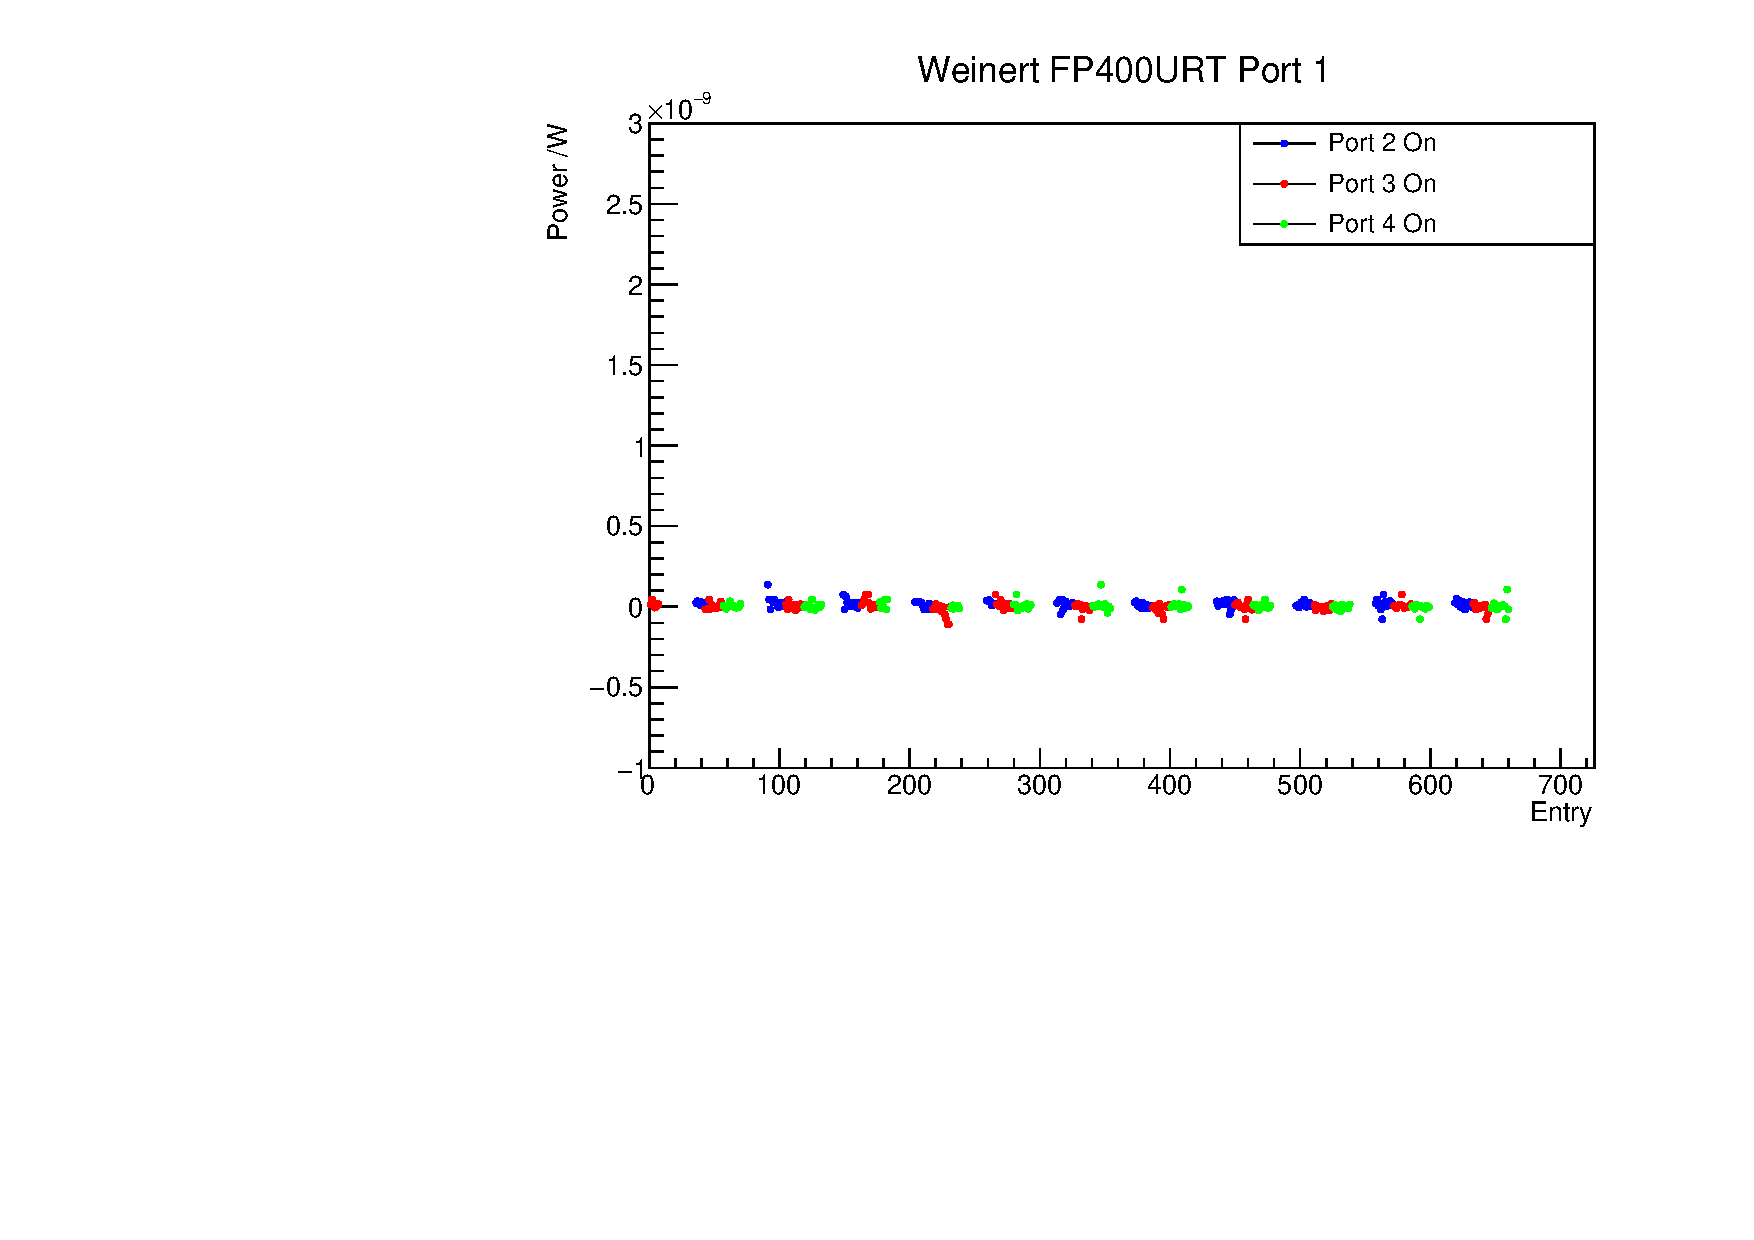
\includegraphics[width=\linewidth]{WeinertFP400URTPort1.pdf}
\subcaption{}\label{fig:weinfp400crosstalkport1}
\end{subfigure}%
\begin{subfigure}{0.5\textwidth}
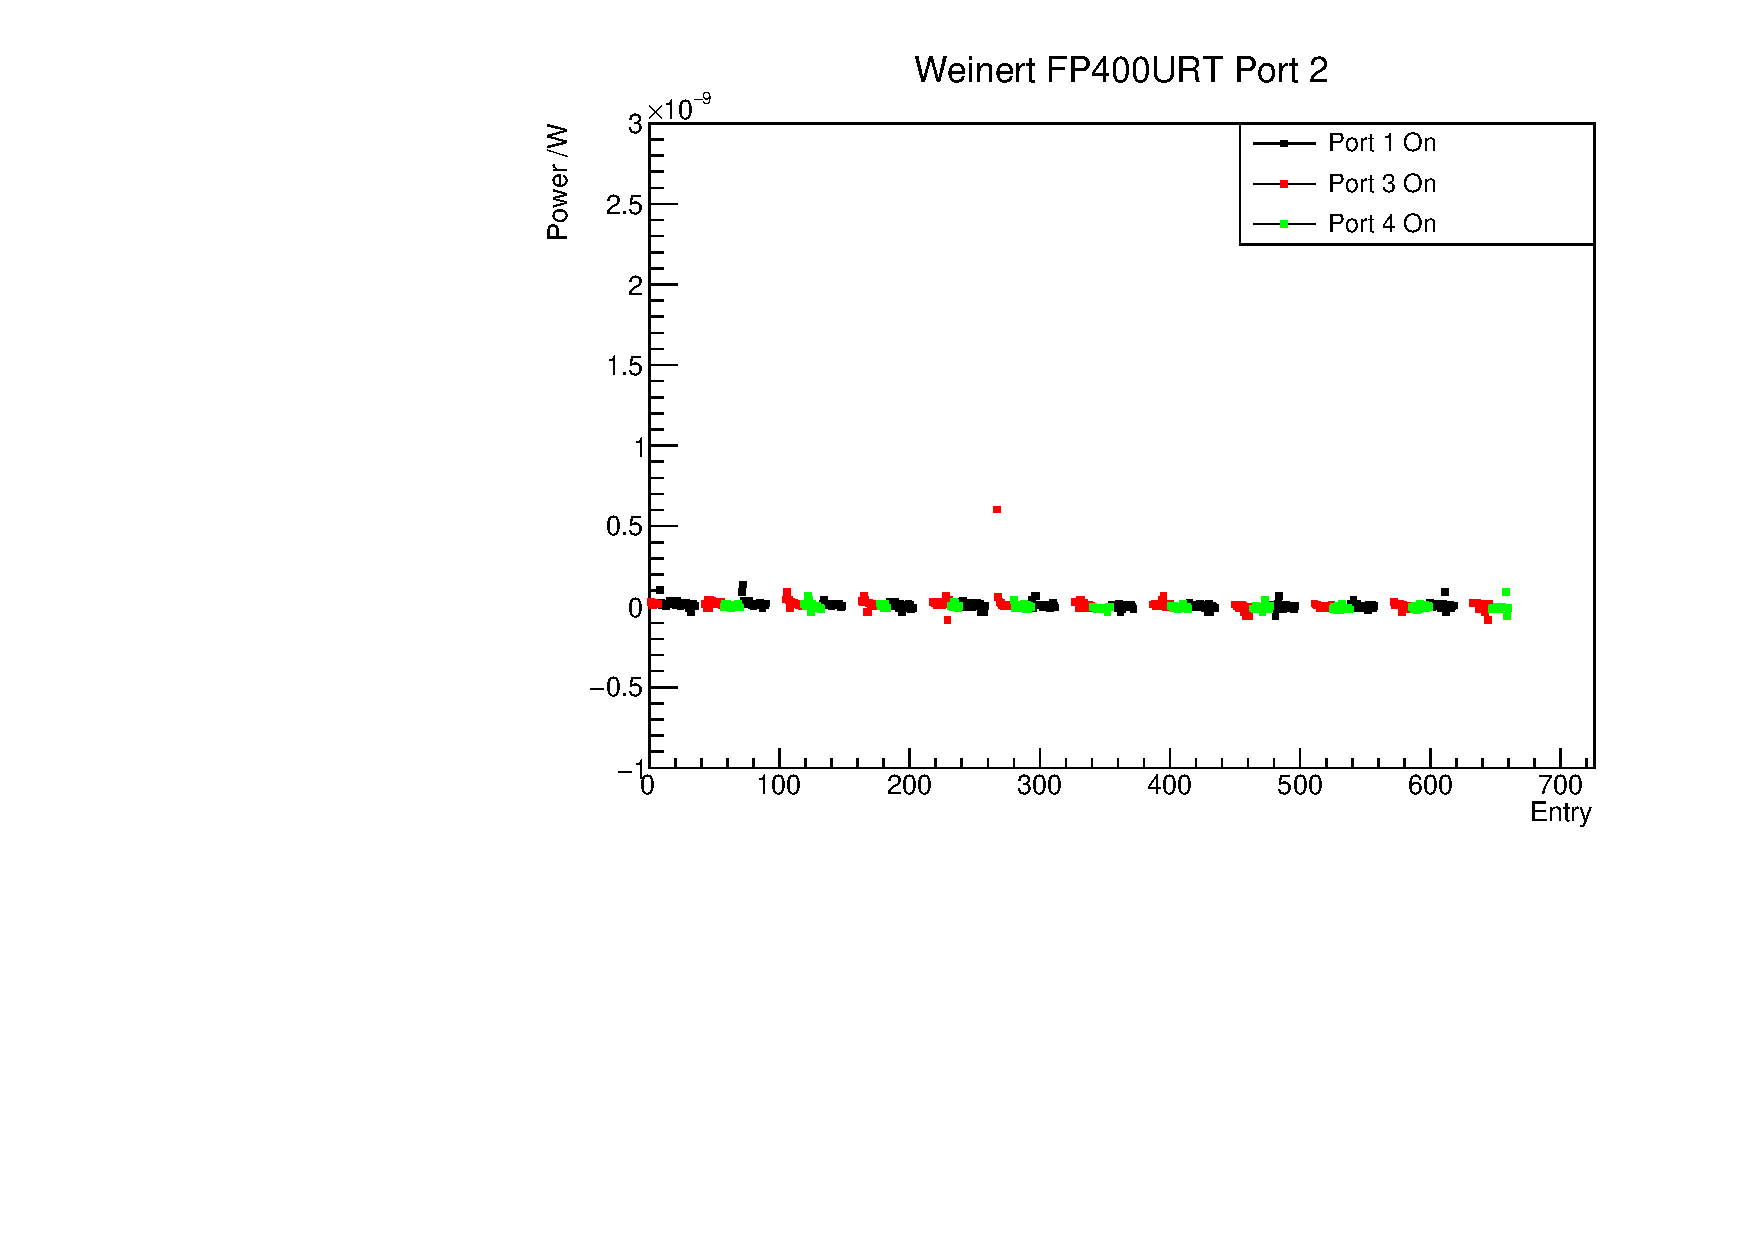
\includegraphics[width=\linewidth]{WeinertFP400URTPort2.pdf}
\subcaption{}\label{fig:weinfp400crosstalkport2}
\end{subfigure}
\\
\begin{subfigure}{0.5\textwidth}
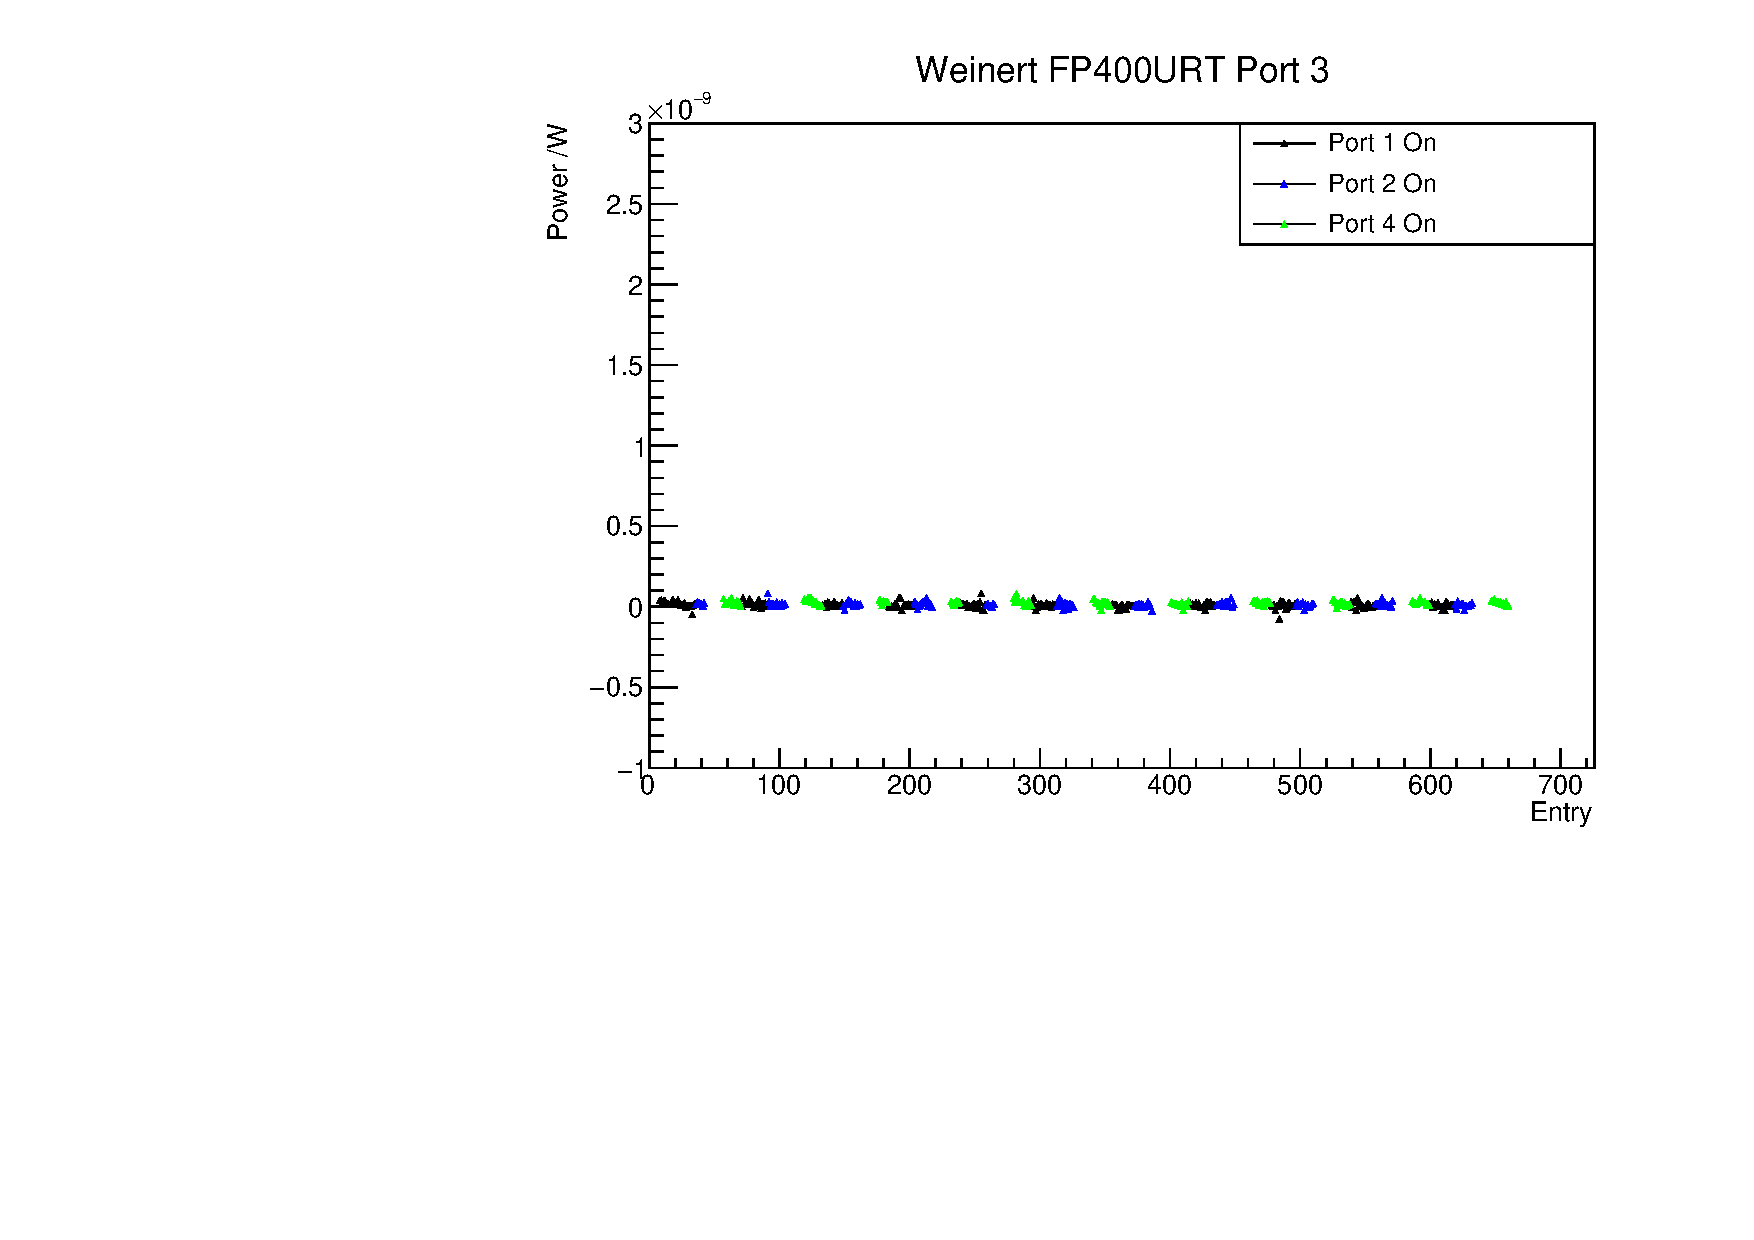
\includegraphics[width=\linewidth]{WeinertFP400URTPort3.pdf}
\subcaption{}\label{fig:weinfp400crosstalkport3}
\end{subfigure}%
\begin{subfigure}{0.5\textwidth}
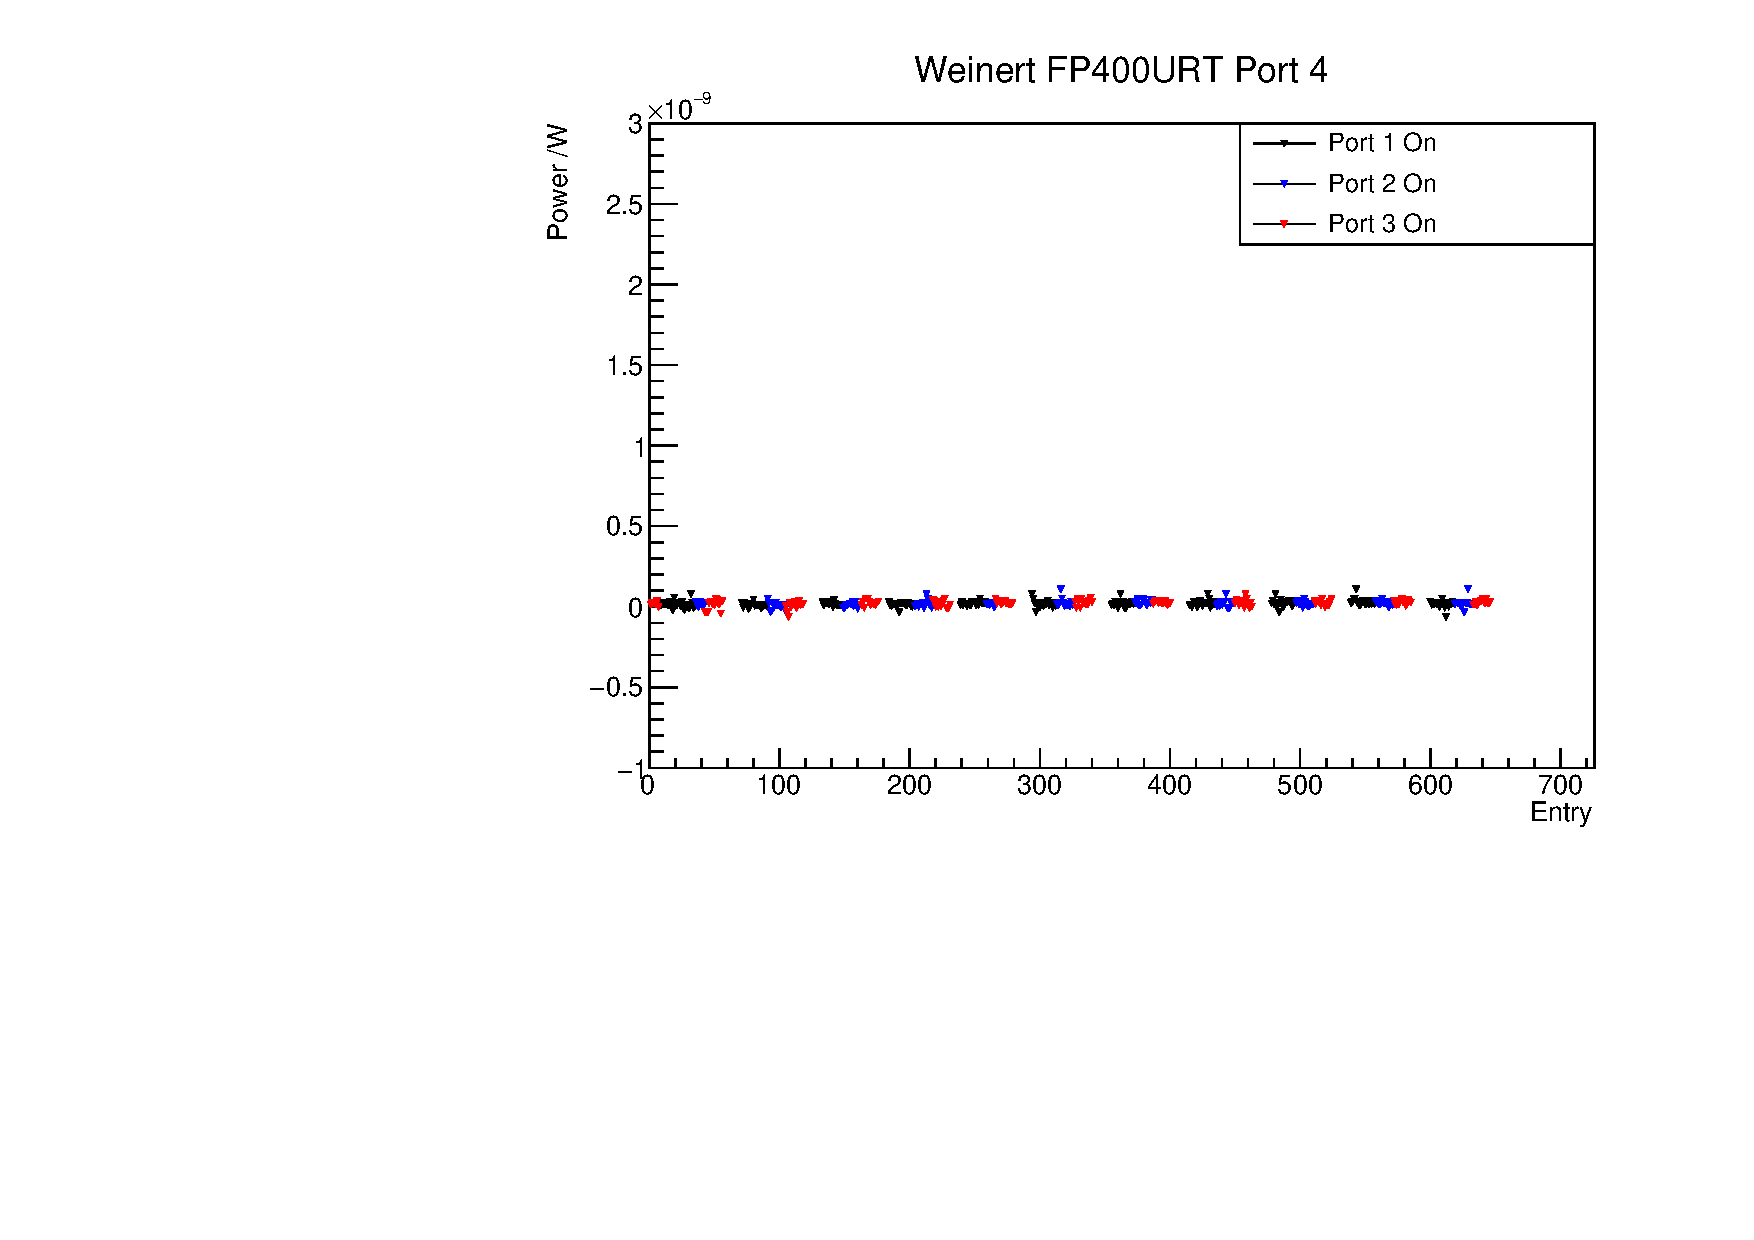
\includegraphics[width=\linewidth]{WeinertFP400URTPort4.pdf}
\subcaption{}\label{fig:weinfp400crosstalkport4}
\end{subfigure}
\caption{Power recorded on a) port 1, b) port 2, c) port 3 and d) port 4 of the Weinert FP400URT switch, when one of the other three ports was illuminated.}\label{fig:weinfp400crosstalk2}
\end{figure}

\clearpage
\newpage
\subsection{Weinert GIF50C}

\begin{figure}[h!]
\centering
\begin{subfigure}{0.5\textwidth}
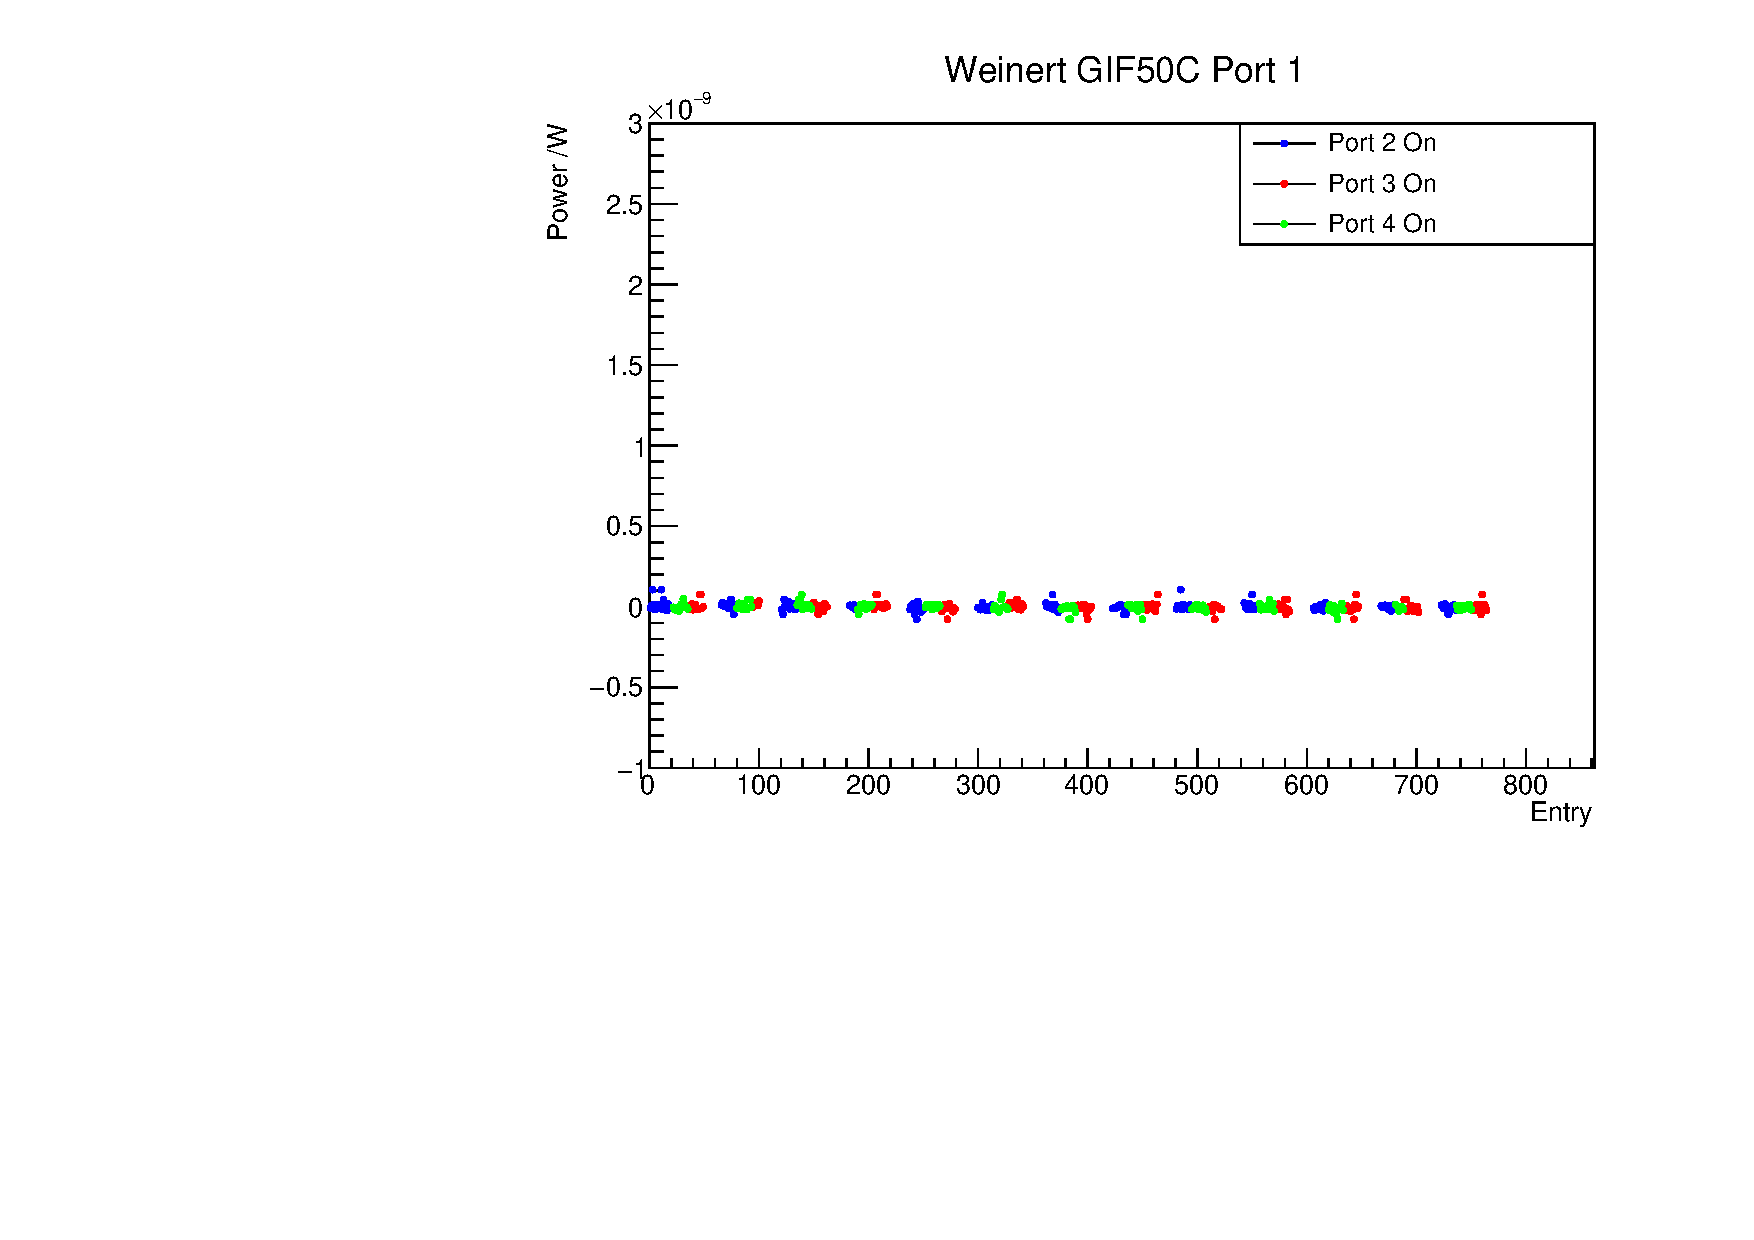
\includegraphics[width=\linewidth]{WeinertGIF50CPort1.pdf}
\subcaption{}\label{fig:weingifcrosstalkport1}
\end{subfigure}%
\begin{subfigure}{0.5\textwidth}
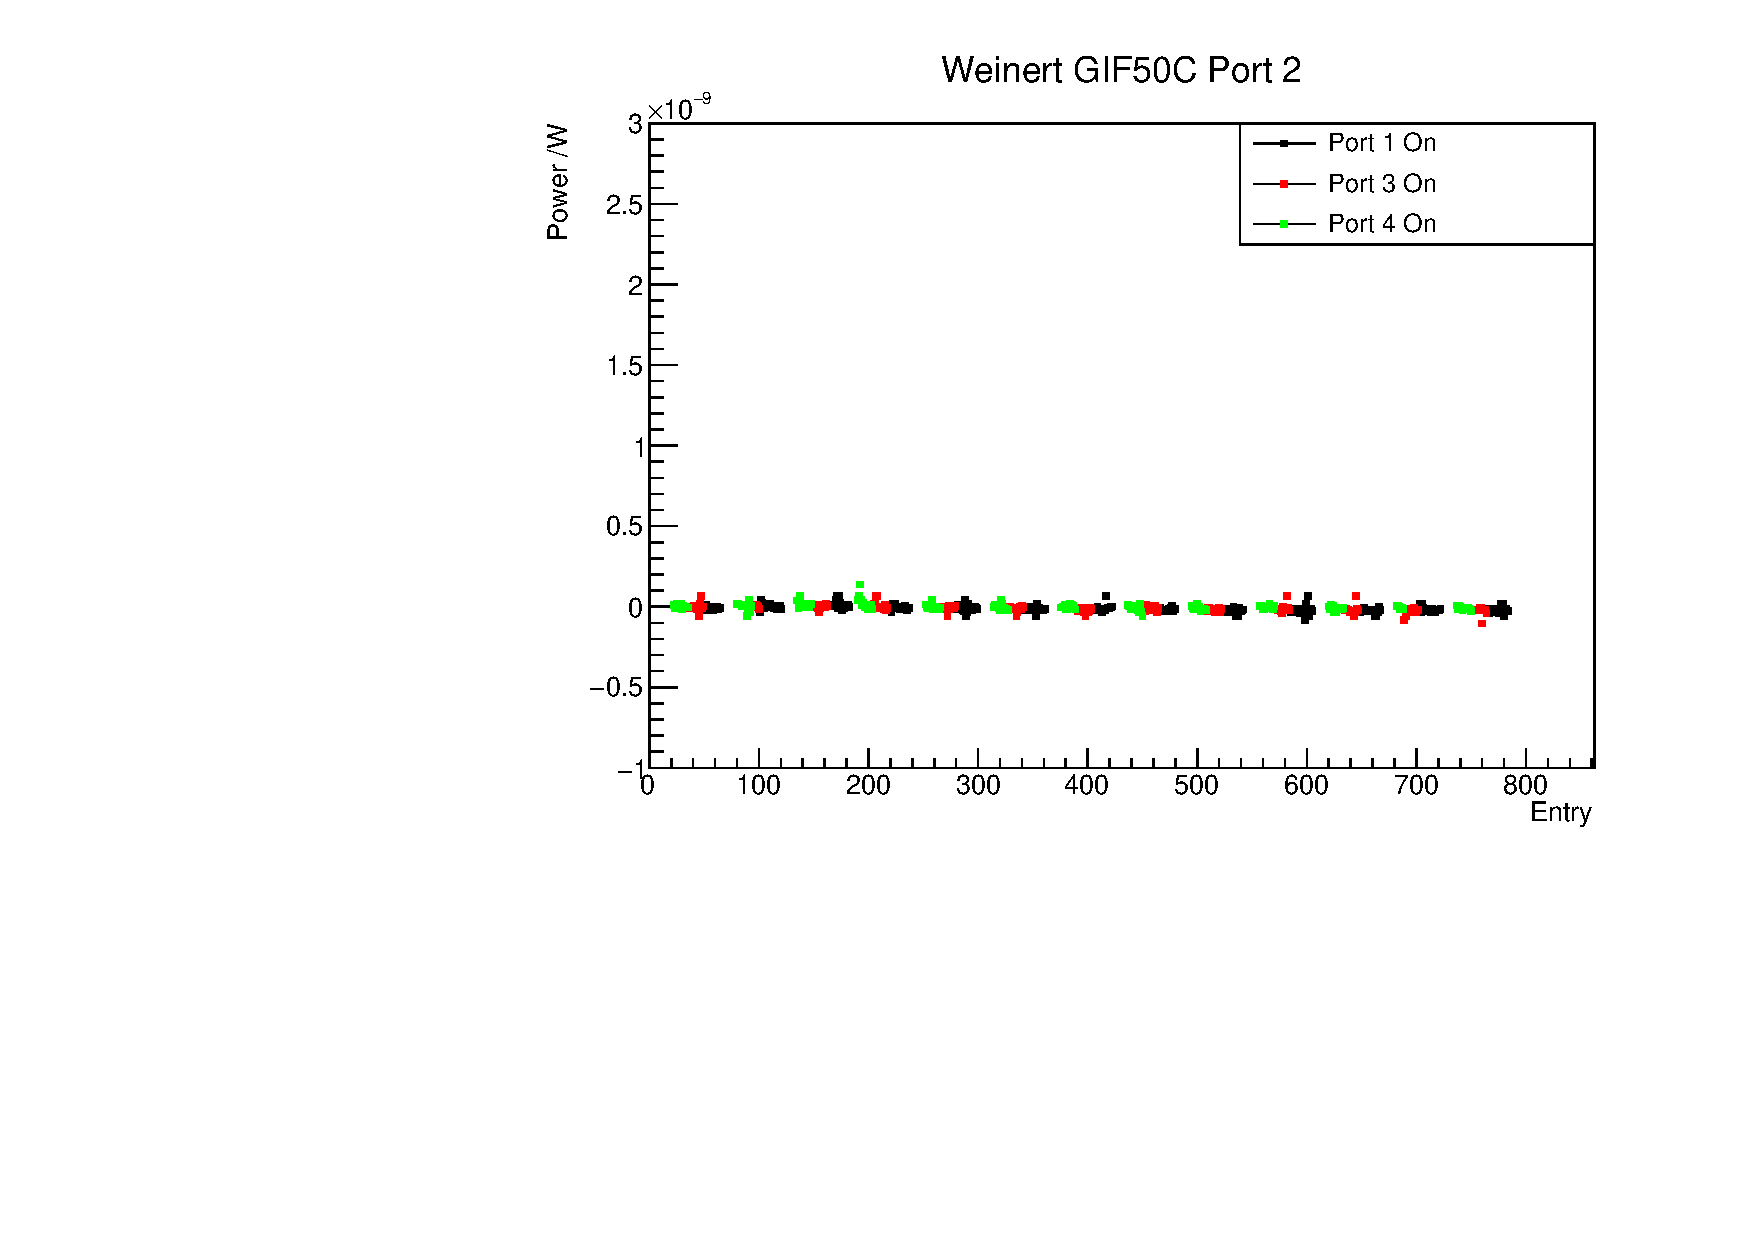
\includegraphics[width=\linewidth]{WeinertGIF50CPort2.pdf}
\subcaption{}\label{fig:weingifcrosstalkport2}
\end{subfigure}
\\
\begin{subfigure}{0.5\textwidth}
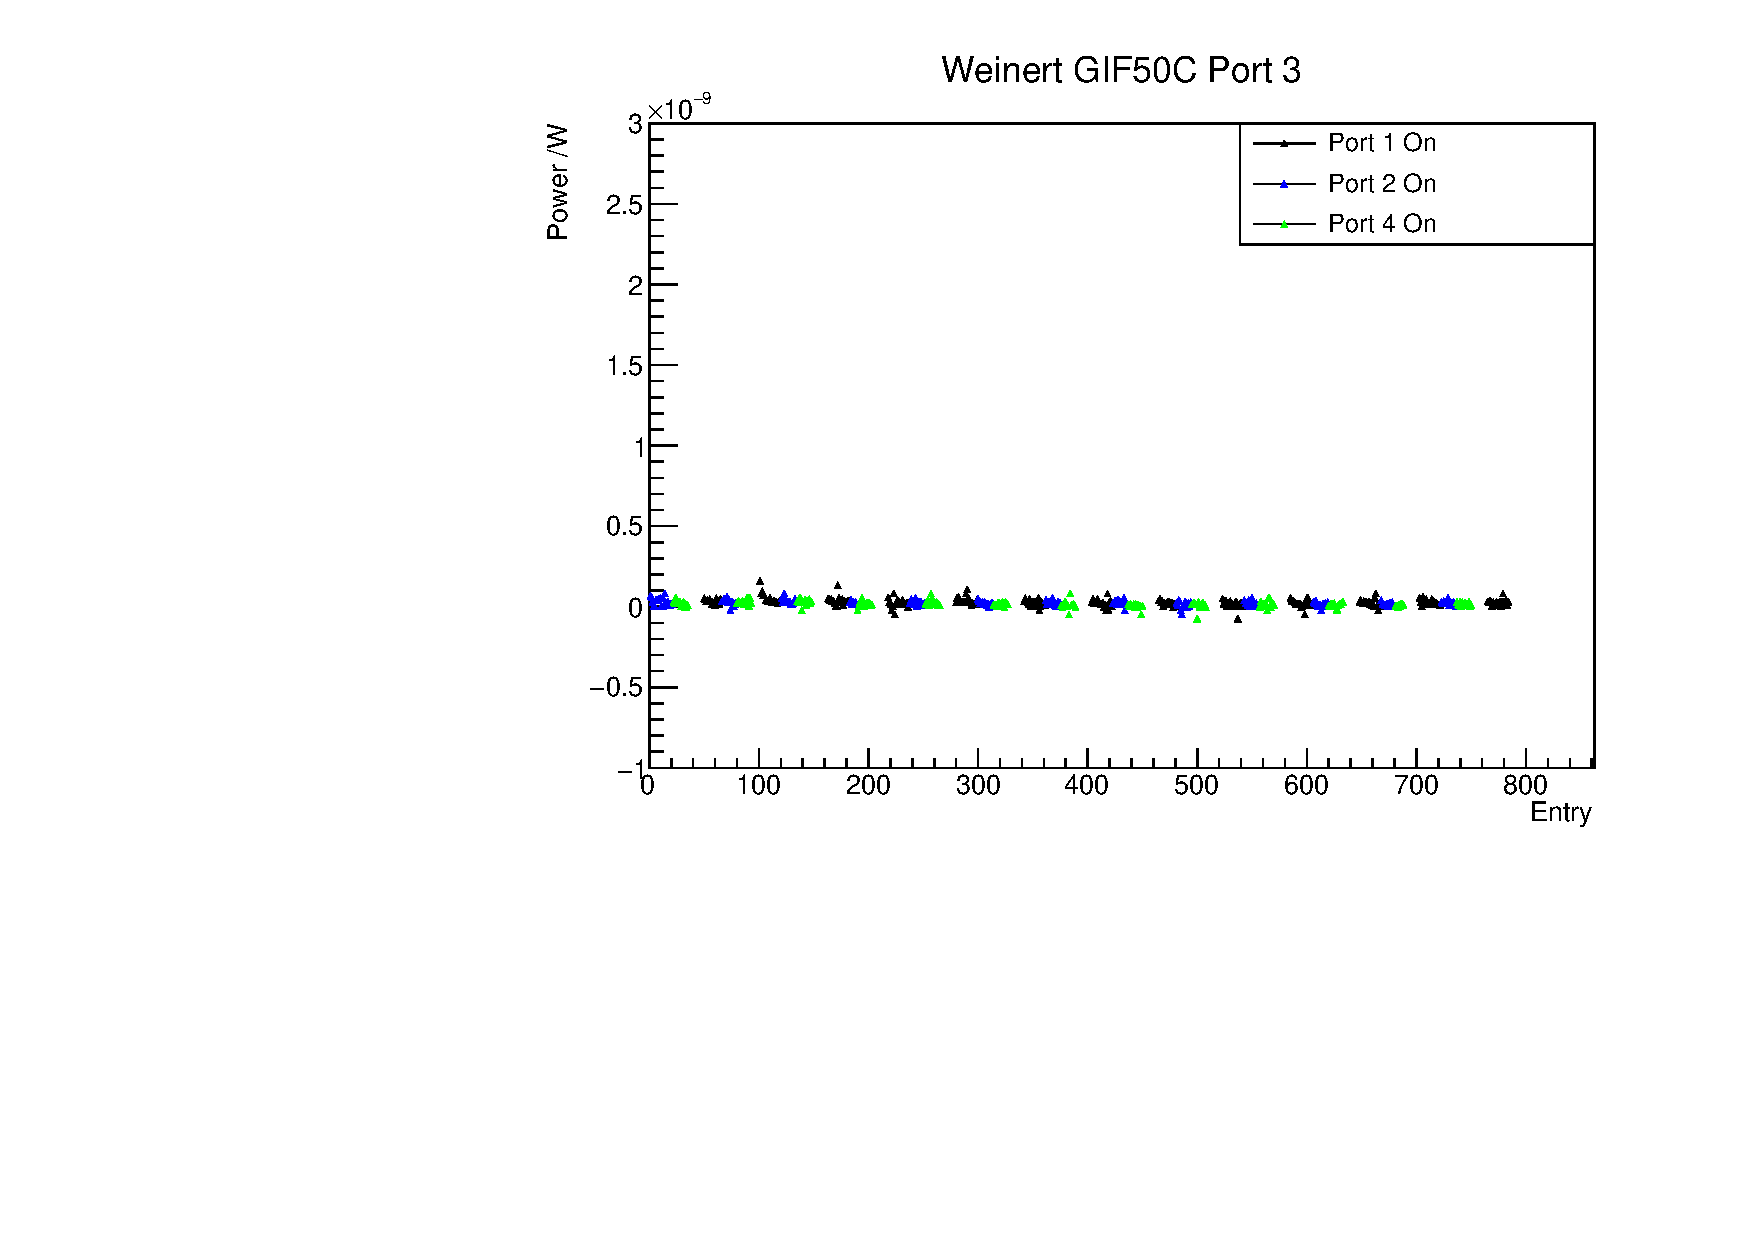
\includegraphics[width=\linewidth]{WeinertGIF50CPort3.pdf}
\subcaption{}\label{fig:weingifcrosstalkport3}
\end{subfigure}%
\begin{subfigure}{0.5\textwidth}
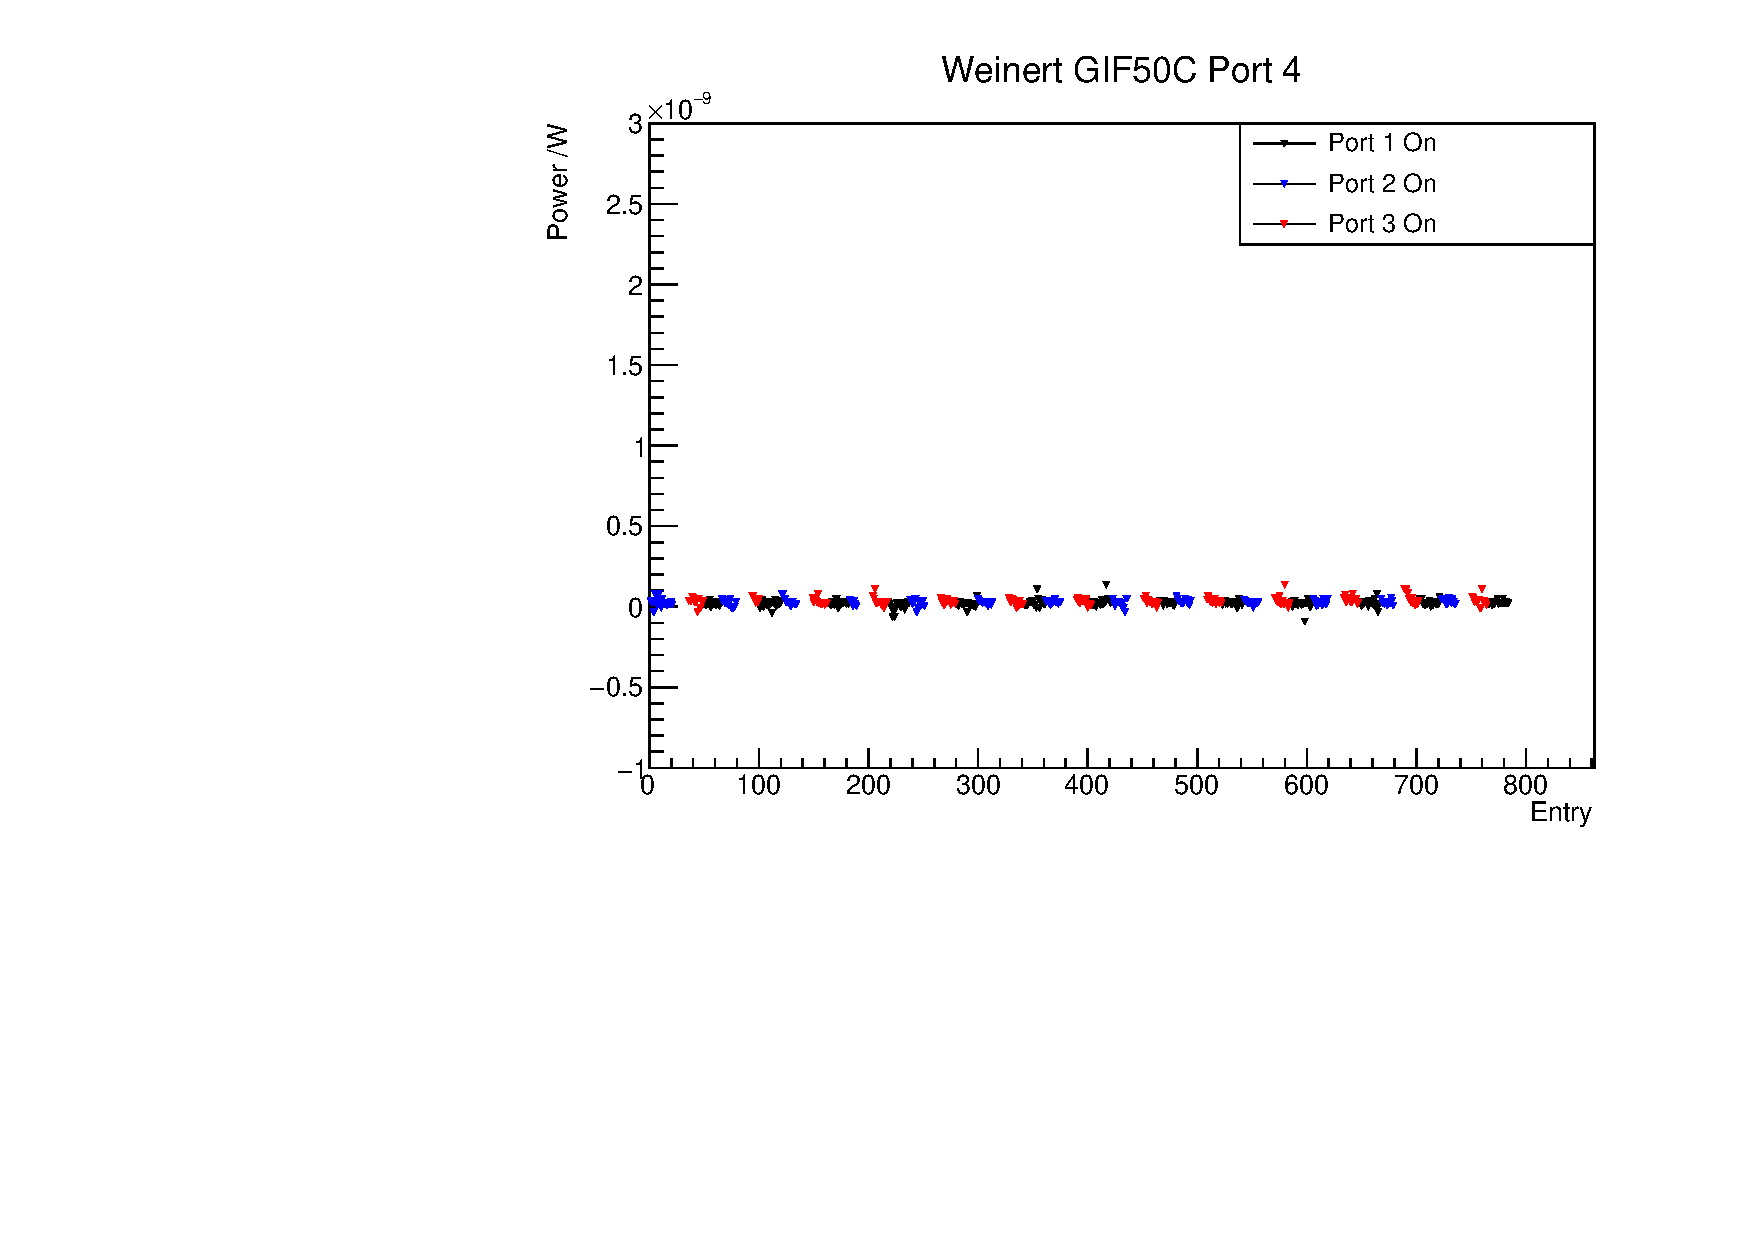
\includegraphics[width=\linewidth]{WeinertGIF50CPort4.pdf}
\subcaption{}\label{fig:weingifcrosstalkport4}
\end{subfigure}
\caption{Power recorded on a) port 1, b) port 2, c) port 3 and d) port 4 of the Weinert GIF50C switch, when one of the other three ports was illuminated.}\label{fig:weingifcrosstalk2}
\end{figure}
\DIFaddbegin 

\clearpage
\newpage

\section{\DIFadd{Fibre Configuration}}\label{app:fibreconfig}

\DIFadd{A more detailed breakdown of the required fibres for both the laser and LED systems is given in \mbox{%DIFAUXCMD
\cref{tab:fibreDetailsLaser} }\hskip0pt%DIFAUXCMD
and \mbox{%DIFAUXCMD
\cref{tab:fibreDetailsLED} }\hskip0pt%DIFAUXCMD
respectively.
}

\begin{table}[h]
\centering
\setlength{\tabcolsep}{4pt}
\rotatebox{90}{
\begin{tabular}{cccccc}
\toprule
Length [m]	&	Connector A	&	Connector B	&	Req. no.	&	Fibre location		&	Injector use	\\ \midrule
76			&	FC/PC (air)		&	FC/PC (water)		&	56				&	Barrel		&	Barrel ID (all)\mbox{%DIFAUXCMD
$^\dagger$
}%DIFAUXCMD
\\
76			&	FC/PC (air)		&	FC/PC (water)		&	8				&	Barrel		&	Bottom ID	\\
76			&	FC/PC (air)		&	FC/PC (water)		&	9				&	Barrel		&	Bottom edge OD collimators	\\
42			&	FC/PC (air)		&	FC/PC (air)		&	56				&	Deck		&	Barrel ID	\\
42			&	FC/PC (air)		&	FC/PC (air)		&	8				&	Deck		&	Bottom ID	\\
42			&	FC/PC (air)		&	FC/PC (air)		&	12				&	Deck		&	All OD collimators	\\
42			&	FC/PC (water)		&	FC/PC (water)		&	8				&	Bottom		&	Bottom ID	\\
10			&	FC/PC (air)		&	FC/PC (water)		&	2				&	Top			&	Top ID		\\
10			&	FC/PC (air)		&	FC/PC (water)		&	3				&	Top			& 	Top edge OD collimators \\
1			&	FC/PC (air)		&	FC/PC (air)		&	8				&	Laser system	&	Before channel split \\
0.64		&	FC/PC (water)		&	FC/PC (water)		&	28				&	Barrel (dead region)	& ID diffuser patch cable	\\
0.64		&	FC/PC (water)		&	FC/PC (water)		&	4				&	Bottom (dead region)	& ID diffuser patch cable	\\
0.56		&	FC/PC (water)		&	FC/PC (water)		&	28				&	Barrel (dead region)	& ID collimator patch cable	\\
0.56		&	FC/PC (water)		&	FC/PC (water)		&	4				&	Bottom (dead region)	& ID collimator patch cable	\\ \midrule
\multicolumn{3}{l}{\mbox{%DIFAUXCMD
$^\dagger$
}%DIFAUXCMD
Staged approach:}			&					&			\\
32			&	FC/PC (air)		&	FC/PC (water)		&	16				&	Barrel	&	Barrel ID (levels 1+2) \\
58			&	FC/PC (air)			&	FC/PC (water)		&	24				&	Barrel	&	Barrel ID (levels 3+4+5)	\\
76			&	FC/PC (air)			&	FC/PC (water)		&	16				&	Barrel	&	Barrel ID (levels 6+7)	\\
\bottomrule
\end{tabular}
}
\caption{\DIFaddFL{List of all required fibres for the laser system with necessary lengths, connector configurations and quantities, along with the location the fibres will be installed and the injectors requiring them. Connector A(B) is defined as that closest to (furthest from) the light source.}}\label{tab:fibreDetailsLaser}
\end{table}


\begin{table}[h]
\centering
\setlength{\tabcolsep}{4pt}
\rotatebox{90}{
\begin{tabular}{cccccc}
\toprule	
Length [m]	&	Connector A	&	Connector B	&	Req. no.		&	Fibre location	& Injector use	\\ \midrule
76			&	FC/PC (air)	&	FC/PC (water)	&	19				&	Barrel			& Bottom OD diff.	\\
76			&	FC/PC (air)	&	Bare (water)	&	84				&	Barrel			& Bottom OD diff. (all)\mbox{%DIFAUXCMD
$^\dagger$
}%DIFAUXCMD
\\
50			&	FC/PC (air)	&	Bare (water)	&	19				&	Top				& Top OD diff. \\
42			&	FC/PC (air)	&	FC/PC (air)	&	19				&	Deck			& Bottom OD diff. \\
42			&	FC/PC (air)	&	FC/PC (air)	&	84				&	Deck			& Barrel OD diff. \\
42			&	FC/PC (air)	&	Bare (water)	&	19				&	Bottom			& Bottom OD diff.	\\
1			&	FC/PC (air)	&	Bare (air)	&	122				&	Crate			& Monitor PMT(s)	\\
0.21		&	FC/PC (air)	&	Bare (air)	&	122				&	Crate 			& Internal patch 1	\\
0.18		&	FC/PC (air)	&	Bare (air)	&	122				&	Crate			& Internal patch 2 \\ \midrule
\multicolumn{3}{l}{\mbox{%DIFAUXCMD
$^\dagger$
}%DIFAUXCMD
Staged approach:}			&					&			\\
32			&	FC/PC (air)	&	Bare (water)	&	24				&	Barrel &	Barrel (levels 1+2) \\
58			&	FC/PC (air)	&	Bare (water)	&	36				&	Barrel &	Barrel (levels 3+4+5)	\\
76			&	FC/PC (air)	&	Bare (water)	&	24				&	Barrel &	Barrel (levels 6+7)	\\
\bottomrule
\end{tabular}
}
\caption{\DIFaddFL{List of all required fibres for the LED system with necessary lengths, connector configurations, quantities, along with the location the fibres will be installed and the injectors requiring them. Connector A(B) is defined as that closest to (furthest from) the light source.}}\label{tab:fibreDetailsLED}
\end{table}
\DIFaddend 


\end{document}
